%!TEX root=dissertation.tex
\chapter{Фотоиндуцированные решетки показателя преломления с сильными периодическими неоднородностями} \label{chapt3}

\section{Введение}
\label{sec:intro}

Из описанных выше технологий получения ВБР становится очевидно, что решетки достаточно высокого качества невозможно получить с помощью длинных фазовых масок, потому что невозможно высококачественно воспроизвести требуемый профиль решетки. Таким образом, требуется технология производства решеток длиннее, чем фазовая маска с дополнительной возможностью чирпирования и контроля фазы. Эта технология почти одновременно была разработана научными группами в Швеции~\cite{Stubbe95} и Англии~\cite{Cole95} в 1995 году. Принцип данной технологии очень прост. Он основан на объединении серий подрешеток, состоящих из многих решеточных плоскостей. В отличии от метода фазовой маски данная технология эффективно основана на смыкании решеточного слоя к решеточному слою, тем самым эффективно усредняя любые неоднородности, возникающие из-за позиционирования при экспозиции. Это имеет место в силу того, что данная плоскость будет облучена $N$ раз, где $N$ есть число плоскостей в каждой подрешетке. Секция решеточных плоскостей как и прежде формируется либо интерферометрически, либо фазовой маской, но каждая из этих решеток транслируется вдоль волокна и положение измеряется с высокой точностью либо glass-encoder'ом, либо еще лучше интерферометром Михельсона с счетчиком полосок, с помощью которого можно достичь точности порядка субнанометров. С помощью такой технологии и точности мониторинга можно получать ВБР длиной несколько метров, что на порядки больше, чем длина типичной фазовой маски.

Опишем ряд технологий, используемых при производстве стандартных и комплексных решеточных структур в оптическом волокне. В зависимости от используемой технологии можно выделить внутренне и внешне записанные решетки. Хотя метод внутренней записи решеток не практичен, его надо принять во внимание для полноты картины. На рис.~\ref{fig4.1} приведена схема первой экспериментальной установки Хилла для записи таких решеток. На сегодняшний день реальное практическое применение получили методы внешней записи решеток: интерферометрический метод, метод фазовой маски и метод <<от точки к точке>>. Они избавлены от недостатков метода внутренней записи.

\begin{figure}
\centering
\includegraphics[width=140px, height=233px]{fig4_1.png}
\caption{Типичная установка, используемая при производстве самоиндуцированных брэгговских решеток облучением аргонового лазера.}\label{fig4.1}
\end{figure}

%%%-----------------------------------------------------------------------------

\subsection{Принцип действия. Феноменологические аспекты записи решеток}
\label{sec:intro_general}

Выше была описана теория, описывающая эффекты УФ-индуцированного изменения ПП в применении к технологически наиболее простыми решетками в волокнах и волноводах. На сегодняшний день существуют коммерческие программы для моделирования волоконных брэгговских решеток в предположении, что изменение ПП происходит линейно. Однако, хотелось бы рассмотреть некоторые ограничения стандартной теории ВБР как таковой и программ для моделирования в частности. Эти ограничения можно разделить на две категории. Первый тип ограничений связан с неполнотой понимания деталей эффектов от неидеальных фазовых масок, используемых совместно с неидеальными лазерными пучками, и все это в комбинации с нелинейным УФ-индуцированным изменением ПП. Честно говоря, это является ограничением не программ моделирования, а ограничением понимания происходящих процессов, которым обладает пользователь. В большинстве случаев практически невозможно измерить экспериментальную мощность УФ излучения и фазовое распределение в ближней зоне фазовой маски. Наилучшей альтернативой является использование независимых характеристик фазовой маски и лазерного пучка, а также векторный дифракционный анализ картины в ближней зоне. Так как подобный анализ чрезвычайно громоздок, его никогда не выполняют на практике.

Другим важным ограничением является то, что на практике все теоретические описания предполагают, что ВБР приводят к незначительным возбуждениям в среде волновода.   Для слабых ВБР в стандартных волокнах и средних решеток в волноводах  с высоким отношением ПП сердцевины и оболочки это является очень хорошим приближением. Однако, оно не срабатывает в случае когда в каком то участке волокна изменение ПП становится настолько большим, что сердцевина волокна локально становится многомодовой. Часто переход между <<возмущенным>> и <<невозмущенным>> режимами крайне велик с изменением в несколько десятков дБ в спектрах прохождения и отражения с десятками или сотнями импульсов УФ излучения при общем облучении длиннопериодной решетки в 25000 импульсов~\cite{HubnerPhD98}. Крайний предел невозмущенного поведения происходит в структурах с фотонными запрещенными зонами, которые во многих случаях могут рассматриваться как очень сильные многомерные решетки.

Волоконные брэгговские решетки, полученные путем записи УФ излучением эксимерного лазера с длиной волны 193 нм, имеющего сравнительно низкое качество пучка, ясно иллюстрирует ряд проблем, связанных с неидеальностью пучка и качества маски наряду с нелинейным изменением ПП~\cite{Hubner97}. Наиболее простая модель роста решетки связывает степень пропускания ВБР со средним изменением ПП в сердцевине волокна. Строго говоря, модель подходит только для случая, когда изменение ПП пространственно локальная аналитическая функция потока УФ излучения. Это имеет место при низкой или средней видимости УФ картины и слабой интенсивности. Эти приближения, как правило, удовлетворяются в случае, когда используется УФ излучение с длиной волны 193 нм, так как последнее имеет низкое качество пучка и для которого не рекомендуется сильная степень фокусировки из-за риска возникновения электрического пробоя в воздухе. Однако, при использовании мощного излучения с длиной волны 248 нм и хорошей пространственной когерентностью, описанные приближения не работают.

Простая феноменологическая модель~\cite{Hubner97} коротко может быть объяснена следующим образом. Когда волокно или волновод облучается однородной УФ интерференционной картиной, изменяется локальный эффективный ПП, $\Delta n$, как функция расстояния, $z$, и УФ потока, $F$, и записывается как
\begin{equation}\label{eq4.1}
  \Delta n(F, z)=\Delta n_{\text{ср}}(F)+\Delta n_{\text{мод}}(F)\sin kz,
\end{equation}
где $k=2\pi /\Lambda$ и $\Delta n_{\text{ср}}$ есть средний эффективный ПП, который может быть рассчитан исходя из измеренного смещения брэгговской длины волны, $\Delta n_{\text{мод}}$– амплитуда модуляции решетки и $\Lambda$ обозначает период решетки. Используя описанные выше предположения, амплитуда модуляции может быть записана как
\begin{equation}\label{eq4.2}
  \Delta n_{\text{мод}}(F)=\left(1/2 \right)\left| \Delta n \left((1+\nu)F \right) - \Delta n \left((1-\nu)F \right)\right|,
\end{equation}
где $\nu$ суть видимость решетки. Рис. \ref{fig4.5} иллюстрирует качество модели.

\begin{figure}
\centering
\includegraphics[width=401px, height=306px]{fig4_5.png}
\caption{Рассчитанная сила решетки на основе измеренного смещения эффективного ПП и простой феноменологической модели записи решетки (сплошная кривая), которая находится в хорошем согласии с результатами прямых измерений (квадратики) в случае, когда видимость, $\nu$, является свободным параметром~\cite{Hubner97}.}\label{fig4.5}
\end{figure}

Сила решетки была оценена, используя в качестве входного параметра среднее изменение эффективного ПП с единственным свободным параметром $\nu$. Наилучшее согласие было получено при $\nu =0,07$. Качество оценки достаточно хорошее, если принять во внимание наличие некой экспериментальной неопределенности. Значение $\nu$ близко к тому, которое можно было бы ожидать при использовании данных о качестве лазерного пучка и данных фазовой маски при френелевском расчете дифракционной картины~\cite{Hubner97}.

В заключении, простая феноменологическая модель  показывает хорошее согласие с результатами серии экспериментов проведенных с различными волокнами и длиной волны облучения 193 нм. В особенности, она объясняет колебания силы решеток, как функции времени облучения, используя при этом полученные значения отклонений среднего ПП. Как и ожидалось, столь простая модель перестает работать, когда фундаментальные предпосылки становятся не верными (т.е. при высокой мощности или видимости интерференционной картины). Однако, она может все еще быть использованной для грубого качественного описания формы кривых силы решеток. Таким образом, эта модель является достаточно удобным инструментом для экспериментаторов, но не особо полезна для детального описания сложных решеток. Возможно, наиболее существенным недостатком модели является необходимость измерения среднего ПП до того, как она будет применена. Причина естественно состоит в том, что подобная простая феноменологическая модель не включает теории основных УФ-индуцированных изменений. Это можно исправить путем объединения данной модели с описанной выше современной микроскопической моделью.

Другим следствием несовершенных условий записи является образование в волокне решеток высокого порядка. Это явление редко наблюдается, так как в большинстве приложений оно не влияет на результат. Однако, такого рода решетки на удивление сильны, как показано на рис.~\ref{fig4.6}. Основной причиной данного явления является присутствие в небольшой степени вкладов 0-го или $\pm 2$-го порядков дифракции от фазовой маски. Это приводит к существенным модуляциям с тем же периодом, что и у фазовой маски~\cite{HubnerPhD98, Malo93} или ее более высокого порядка (полуцелого порядка по сравнению с <<нормальной>> решеткой). По тем же причинам можно ожидать, что это приведет к появлению решеток порядка 0,5 (субгармоника), но так как они, как правило, лежат в районе 3,1 мкм, они никогда не наблюдаются.
\begin{figure}
\centering
\includegraphics[width=341px, height=225px]{fig4_6.png}
\caption{Наблюдение решеток более высокого порядка, появившихся из-за влияния нелинейного УФ-индуцированного изменения ПП как функции потока совместно с разницей в дифракционных порядках $\pm 1$ от фазовой маски \cite{HubnerPhD98}. В районе 625 нм и 1050 нм наблюдаются нецелочисленные порядки решеток от интерференции между $\pm 1$ порядками и или $0$, или $\pm 2$ порядками дифракции от фазовой маски \cite{Dyer95}.}\label{fig4.6}
\end{figure}
Даже если у вас идеальная фазовая маска, существует некоторая доля решеток с более высоким целочисленным порядком. Это имеет место в силу нелинейного УФ-индуцированного изменения ПП как функции потока (а для импульсных лазеров и как функции интенсивности).

%%%-----------------------------------------------------------------------------

На рис.~\ref{fig4.7} представлена установка для получения волоконных брэгговских решеток. В качестве источника УФ излучения используется удвоенный по частоте аргоновый лазер с длиной волны 244 нм. Такая длина волны необходима из-за того, что она находится близко от длины волны максимальной фоточувствительности Ge/Si оптического волокна. Для получения интерференционной картины используется однородная фазовая маска стандартной длины 2 см. Волокно крепится на трансляционной подставке с помощью высокоточных зажимов, обеспечивающих постоянство (неизменность) расстояния между волокном и фазовой маской при движении вдоль всей подставки (основы, опоры). Волокно непрерывно транслируется с постоянной скоростью вдоль продольной оси. Движение волокна относительной интерференционной картины измеряется с помощью дифференциального He-Ne (632,8 нм) интерферометра производства Zygo. Данный интерферометр дает на выходе значение в виде 32-битного числа, представляющего собой относительное положение с точностью $\thicksim 1,24$ нм.
\begin{figure}
\centering
\includegraphics[width=424px, height=266px]{fig4_7.png}
\caption{Типичная схема записи длиннопериодных волоконных брэгговских решеток.}\label{fig4.7}
\end{figure}
Если мы начнем сканировать волокно с постоянно включенным УФ излучением, то не запишем никакой решетки, даже несмотря на то, что интерференционная картина с фазовой маски была получена. Однако, если УФ излучение модулировать (стробоскопировать) с временным периодом, равным периоду генерируемой  маской интерференционной картины относительно постоянной скорости, с которой сканируется подставка, решетка будет записана в сердцевине волокна. Другими словами для генерирования решетки УФ излучение необходимо включать и выключать тогда, когда выравнивается интерференционная картина с фазовой маски и уже записанная интерференционная картина в сердцевине волокна. Для достижения этого значение положения с интерферометра сравнивается со значением на контроллере и при достижении определенной пропорции контроллер включает (пропускает) УФ излучение к маске. В этом случае полученная на маске интерференционная картина совпадает с уже записанной на волокне. Включение или выключение УФ излучения в определенный момент времени зависит от состояния сигнала контроля модуляции генерируемого контроллером и соответственно используемого для контроля состояния акустооптического модулятора (АОМ). На рис.~\ref{fig4.7}  показан принцип записи таких решеток. Из-за того, что основа движется с постоянной скоростью слева направо, процесс записи проиллюстрирован в точке записи решетки, а не в самом начале. Как было сказано выше, УФ пучок периодически модулирован согласованно с движением волокна. Таким образом, каждая последующая экспозиция генерирует периодическое изменение ПП выровненное и перекрывающее предыдущую экспозицию. Таким образом, изменение коэффициента преломления, представляющее собой отдельную полоску в решетке, построена на кумулятивном эффекте многократной экспозиции через различные части интерференционной картины, возникающие при движении волокна. В связи с этим необходимая для формирования решетки мощность распределяется между большим числом экспозиций таким образом, что каждая отдельная экспозиция может быть относительно малой мощности и фаза между двумя последовательными экспозициями может быть проконтролирована так, что чирп, апподизация и дискретные фазовые скачки могут быть внедрены в структуру решетки.

%%%-----------------------------------------------------------------------------

\subsection{Метод формирования брэгговских решеток в волокне}

\subsubsection{Метод интерференции пучков}

Интерферометрический метод впервые был продемонстрирован группой Мелтца~\cite{Meltz89}. Они использовали интерферометр с расщеплением амплитуды для получения волоконной брэгговской решетки. Их экспериментальная установка показана на рис.~\ref{fig4.8}. Используя нелинейный кристалл они удвоили частоту лазера на красителях с эксимерной накачкой с первоначальной длиной волны в диапазоне 486-500 нм и получили источник УФ излучения с длиной волны 244 нм и приемлемой длиной когерентности (критический параметр в данном методе). УФ излучение было разделено на два пучка одинаковой интенсивности и объединены для получения интерференционной картины, нормальной к оси волокна. Пара цилиндрических линз фокусировала излучение на волокне и результирующая фокальная линия составляла 4 мм в длину и 125 мкм в ширину. Также использовался источник с широким спектром и монохроматор с высоким разрешением для мониторинга спектра отражения и прохождения решетки. На врезке рис.~\ref{fig4.8} также показаны спектры прохождения и отражения решетки, записанной в волокне с диаметром сердцевины 2,6 мкм, легированного 6,6 мол.\% GeO$_2$ после 5 минут экспозиции излучением на 244 нм со средней мощностью 18,5 мВт. Длина области экспозиции была в районе 4,2-4,6 мм.

\begin{figure}
\centering
\includegraphics[width=429px, height=206px]{fig4_8.png}
\caption{Интерферометр Мелтца с амплитудным расщеплением~\cite{Meltz89}.}\label{fig4.8}
\end{figure}

В обычном интерферометре, таком, как на рис.~\ref{fig4.8}, УФ лазерное излучение разделяется на два пучка, которые затем объединяются, но претерпев перед этим в каждом из оптических каналов различное число отражений. Поэтому интерферирующие пучки (волновые фронты) требуют различной (латеральной) ориентации. Для лазерных пучков со слабой пространственной когерентностью это приводит к низкому качеству интерференционной картины. Эта проблема решается путем введения в один из каналов дополнительного зеркала. Схема дана на рис.~\ref{fig4.9}. Так как теперь количество отражений в каждом канале одинаково, два интерферирующих на волокне пучка становятся идентичными.

\begin{figure}
\centering
\includegraphics[width=454px, height=212px]{fig4_9.png}
\caption{Улучшенная версия интерферометра с амплитудным расщеплением, где использовано дополнительное зеркало для получения одинакового числа отражений, т.о. исключая различную латеральную ориентацию интерферирующих пучков. Этот интерферометр применим для систем, где источник обладает низкой пространственной когерентностью, такой как эксимерный лазер.}\label{fig4.9}
\end{figure}

Так как период ВБР совпадает с периодом полос в интерференционной картине, то период решетки дается соотношением

\begin{equation}\label{eq4.5}
\Lambda =\lambda_w /2\sin \phi,
\end{equation}
где $\lambda_w$ - длина волны падающего излучения, $\phi$ - угол падения (см. рис. \ref{fig4.9}). Если учесть, что $ \lambda_B =2n_\Lambda$, можно записать

\begin{equation}\label{eq4.6}
\lambda_B = \lambda_w /\sin\phi,
\end{equation}
где $n_{\text{эфф}}$ --- эффективный коэффициент преломления сердцевины волокна. Видно, что брэгговская длина волны решетки может быть изменена путем варьирования $\lambda_w$ и (или) $\phi$. Выбор $\lambda_w$ ограничен диапазоном фоточувствительности волокна, тогда как особых ограничений на выбор $\phi$ нет.

Одним из преимуществ интерферометрического метода является возможность введения дополнительных оптических компонентов в канал(ы) интерферометра, что позволяет изменить волновой фронт интерферирующих пучков. На практике ввод одной или нескольких цилиндрических линз в один или оба канала интерферометра приводит к чирпированию решетки с широкими возможностями варьирования параметрами~\cite{Bennion96}. Одним из важных преимуществ интерферометрического метода с амплитудным расщеплением является возможность записи решеток на любой длине волны. Это достигается за счет возможности изменения брэгговской длины волны путем вариации угла пересечения УФ пучков. Этот метод также позволяет производить решетки практически любой длины. Основным недостатком метода является его крайняя чувствительность к механическим вибрациям. Субмикронные изменения положений оптических компонент приводит к расплыванию интерференционной картины. Кроме того, качественные решетки могут быть получены только при использовании лазерных источников с хорошей пространственной и временной когерентностью и высокой стабильностью длины волны и выходной мощности.

При производстве решеток интерферометры с расщеплением волнового фронта не стали столь популярны, как интерферометры с амплитудным расщеплением, однако они имеют ряд полезных преимуществ. Приведем два примера интерферометров с расщеплением волнового фронта: призменный интерферометр~\cite{Kashyap90, Egglton94} и интерферометр Ллойда~\cite{Limberger93}. Экспериментальная установка для записи решеток с помощью интерферометра Ллойда показана на рис.~\ref{fig4.10}. Он состоит из диэлектрического зеркала, которое направляет половину УФ пучка на волокно, расположенного перпендикулярно зеркалу. Записывающий пучок центрирован на пересечении поверхности зеркала и волокна. Пересечение прямого УФ пучка и его отклоненной части приводит к образованию интерференционной картины, нормальной к оси волокна. Обычно для фокусирования интерференционной картины (полос) на сердцевине волокна используются цилиндрические линзы. Так как половина падающего пучка претерпела отражение, ширина интерференционной картины равна половине ширины пучка. По той же причине интерференционные полосы могут иметь разное качество. Дифракционные эффекты от краев диэлектрического зеркала могут препятствовать получению качественной дифракционной картины.

\begin{figure}
\centering
\includegraphics[width=441px, height=291px]{fig4_10.png}
\caption{Схема интерферометра Ллойда с расщеплением волнового фронта.}\label{fig4.10}
\end{figure}

Схема призменного интерферометра показана на рис.~\ref{fig4.11}. Призма сделана из высокочистого кварца. Падающий УФ пучок, претерпев отражения от правой (см. рис.~\ref{fig4.11}) границы призмы, объединяется с неотраженной частью пучка, вследствие чего на выходной границе призмы мы получаем интерференционную картину. Для фокусирования линий на фоточувствительной сердцевине волокна используются цилиндрические линзы. Данный тип интерферометра достаточно стабилен в силу того, что разница оптических путей появляется внутри призмы и избавлена от действия внешних вибраций. Время записи решеток таким интерферометром составляет порядка 8 часов. Одним из недостатков данной системы является геометрия интерферометра. Для того чтобы получить интерферограмму наложением пучка самого на себя необходимо, чтобы интерферировали различные части пучка, что в свою очередь требует от источника УФ излучения хорошей пространственной когерентности.

\begin{figure}
\centering
\includegraphics[width=443px, height=333px]{fig4_11.png}
\caption{Схема призменного интерферометра с расщеплением волнового фронта.}\label{fig4.11}
\end{figure}

Основным преимуществом интерферометра с расщеплением волнового фронта является его базирование на одной оптической компоненте. Это значительно снижает чувствительность системы к механическим вибрациям. Кроме того, малые расстояния разделения УФ пучков уменьшает искривление волнового фронта, вызванного неоднородностью воздушной среды и разницей температур в среде. Наряду с этим, система может легко вращаться для изменения угла пересечения пучков и соответствующего изменения длины волны решетки. Основным недостатком является ограничение по длине решетки, равной в пределе полуширине пучка. Недостатком также является ограниченное изменение брэгговской длины волны вследствие физических ограничений интерферометра. При увеличении угла пересечения разница между оптическими путями двух пучков также увеличивается, поэтому длина когерентности пучков ограничивает диапазон изменения брэгговской длины волны.

%%%-----------------------------------------------------------------------------

\subsubsection{Метод фазовой маски}

Одним из наиболее эффективных методов записи решеток считается метод фазовой маски~\cite{Hill93}. В этом методе для пространственной модуляции оптического пучка используется дифракционный оптический элемент – фазовая маска, изображенная на рис.~\ref{fig4.12}. Фазовая маска может быть получена голографически или методом электронно-лучевой литографии. Первый метод более точный, чем второй. Решетка фазовой маски представляет собой одномерную структуру на поверхности высокочистой кварцевой пластинки, прозрачной для УФ излучения. Профиль решетки выбирается таким образом, чтобы при облучений фазовой макси УФ излучением, дифрагирующий пучок нулевого порядка был подавлен до нескольких процентов (как правило, менее 5 \%) проходящего излучения. В то время как дифрагирующие пучки плюс и минус первых порядков имели максимальную мощность и составляли более 35 \% от общей прошедшей мощности излучения. Интерференционная картина в ближней зоне получается за счет интерференции дифрагирующих пучков плюс и минус первого порядка. Период полос равен половине длины маски. Интерференционная картина производит модуляцию коэффициента преломления в фоточувствительной сердцевине волокна, расположенного в непосредственном контакте или на небольшом расстоянии от фазовой маски (см. рис.~\ref{fig4.12}). При необходимости для фокусирования полос используются цилиндрические линзы.

\begin{figure}
\centering
\includegraphics[width=415px, height=246px]{fig4_12.png}
\caption{Схема иинтерферометрической установки для записи брэгговской решетки в оптоволокне с помощью фазовой маски.}\label{fig4.12}
\end{figure}

Использование фазовых масок значительно упрощает систему для записи волоконных решеток. Простота в основном основана на использовании лишь одного оптического элемента, что делает данный метод очень надежным и стабильным. Так как волокно располагается непосредственно за фазовой маской, проблема чувствительности к механическим вибрациям минимизируется. В силу геометрии низкая временная когерентность не влияет на записывающую способность системы (в отличие от интерферометрического метода).

В данном методе в качестве УФ источника обычно используют эксимерный KrF лазер. Источники УФ излучения, как правило, имеют низкую пространственную и временную когерентность. Однако наличие пространственной когерентности значительно улучшает качество производства ВБР методом фазовой маски. Рассмотрим простую схему на рис.~\ref{fig4.13}. Пусть сердцевина волокна находится на расстоянии $h$ от фазовой маски. Дифрагирующие пучки первого порядка (плюс и минус) интерферируют с образованием интерференционной картины на волокне. Они исходят из различных частей фазовой маски, находящихся на расстоянии $d$ друг от друга. Так как расстояние до волокна для обоих пучков одинаково, требование временной когерентности не критично для получения контрастной интерференционной картины. С другой стороны, при увеличении расстояния $h$ пространство $d$ между пучками также увеличивается. В этом случае требование высокой пространственной когерентности становится критичным. Если расстояние $h$ превысит длину пространственной когерентности падающего УФ излучения, мы можем вообще не получить интерференционной картины. Этот вопрос хорошо изучен в работе~\cite{Dyer96}.

\begin{figure}
\centering
\includegraphics[width=416px, height=222px]{fig4_13.png}
\caption{Простая схема фазовой маски для записи брэгговской решетки в оптоволокне. Дифракционные пучки плюс и минус первого порядка интерферируют в сердцевине волокна, расположенного на расстоянии $h$ от маски.}\label{fig4.13}
\end{figure}

%%%-----------------------------------------------------------------------------

\subsubsection{Метод <<от точки к точке>>}

Техника получения ВБР методом <<от точки к точке>>~\cite{Malo93} основана на дискретной локальной модуляции коэффициента преломления. Иными словами, в данном методе каждый штрих наносится отдельно путем облучения сердцевины волокна сфокусированным одиночным импульсом эксимерного лазера. Пучок УФ излучения проходит через диафрагму (щель), затем фокусирующая линза строит изображение щели на сердцевине оптического волокна, что в свою очередь ведет к локальному повышению коэффициента преломления в сердцевине. Схема установки показана на рис.~\ref{fig4.14}.

\begin{figure}
\centering
\includegraphics[width=431px, height=225px]{fig4_14.png}
\caption{Схема установки для записи ВБР методом <<от точки к точке>>.}\label{fig4.14}
\end{figure}

Затем волокно перемещается на расстояние периода решетки $\Lambda$ и процесс облучения повторяется. Наиболее существенным в данном методе является высокая стабильность и субмикронная точность трансляционной системы.

Основным преимуществом метода <<от точки к точке>> является его гибкость в отношении изменения параметров ВБР. Не представляет никакой сложности изменить длину решетки, период нанесения штрихов и, соответственно, построит необходимый спектральный отклик. Этот метод позволяет получить пространственные~\cite{Hill90} и поляризационные~\cite{Hill91} модовые конвертеры, которые имеют период решетки от десятков микрометров до десятков миллиметров. Кроме того, так как мы можем изменять интенсивность облучения на каждом штрихе, то довольно просто получить необходимый профиль модуляции коэффициента преломления и соответствующий спектральный отклик решетки.

Основным недостатком метода является его крайняя утомительность. В силу того, что это пошаговая процедура, он требует сравнительно много времени. Кроме того, из-за температурных эффектов и (или) напряжений в волокне возможны ошибки в периоде решетки. Поэтому таким методом в основном записывают короткие решетки. Типичный период решетки для отражения первого порядка на длине волны 1550 нм равен 530 нм. Из-за малого периода и сложности фокусировки ВБР первого порядка на 1550 нм еще никому не удалось сделать. Группе Мало~\cite{Malo93} этим методом удалось получить только ВБР 2 и 3 порядков с периодом 1 мкм и 1,5 мкм соответственно.

В итоге приведем кратко положительные и отрицательные стороны каждого метода.
{\footnotesize
\begin{flushleft}
\begin{tabular}{|l|l|l|}
\hline
\textbf{Метод}&\textbf{Минусы}&\textbf{Плюсы}
\\

\hline
Интерференции &
\begin{tabular}{l}
1. Высокая когерентность источника \\
2. Сложность юстировки \\
3. Большое количество компонент
\end{tabular}
&
\begin{tabular}{l}
1. Гибкость к изменению \\
параметров решетки
\end{tabular}
 \\ &&
\\

\hline
Фазовой маски &
\begin{tabular}{l}
1. Фиксированные параметры решетки \\
2. Много компонент, но меньше \\ чем у интерферометрического метода
\end{tabular} &
\begin{tabular}{l}
1. Повторяемость решеток \\
2. Точность параметров
\end{tabular}
\\

\hline
\glqq От точки к точке\grqq &
\begin{tabular}{l}
1. Высокие требования к подвижкам \\
2. Только для длиннопериодных решеток
\end{tabular}
&
\begin{tabular}{l}
1. Любые параметры \\ длиннопериодных ВБР \\
2. Решетки с модули- \\рованным периодом
\end{tabular} \\
\hline
\end{tabular}
\end{flushleft}
}

%%% ----------------------------------------------------

\subsection{Специфика использования ВБР в лазерных системах высокой мощности}
\label{sec:intro_specific}

Здесь текст специфики ВБР в кВт лазере.

% =================================================================
\section{Теоретическое исследование ВБР в случае сильных периодических неоднородностей}
\label{sec:fbg_strong_periodic_structure}
% =================================================================

\subsection{Классическое описание среды со слабыми периодическими неоднородностями}

Рассмотрим среду, в которой скорость распространения волны является периодической функцией какой-либо одной пространственной координаты (например, $x$):
\begin{equation}\label{1.1}
c^2=c_0^2[1-\mu \cos(2Kx)],
\end{equation}
где $K=2\pi/\Lambda$ ($\Lambda$ -- пространственный период решетки). Будем считать, что неоднородность мала, иными словами $\mu \ll 1$. В этом случае уравнение для волны, распространяющейся вдоль оси $x$, можно записать в виде
\begin{equation}\label{1.2}
\frac{\partial^2 u}{\partial x^2}-\frac{1}{c_0^2}\left[1+\mu\cos(2Kx) \right]\frac{\partial^2 u}{\partial t^2}=0.
\end{equation}
Предположим, что зависимость от времени -- гармоническая, т. е. $u = \qquad =A(x)\exp(i\omega t)$. Тогда для амплитуды $A$ получим уравнение:
\begin{equation}\label{1.3}
\frac{d^2 A}{dx^2}+k^2\left[1+\mu\cos(2Kx) \right]A=0,
k^2=\omega^2/c_0^2.
\end{equation}
\begin{utv}
При $k_0=K$ дисперсионная кривая $\omega(k_0)$ испытывает разрыв. Запрещенная полоса частот имеет ширину $\Delta\omega=\mu\omega_0/2$.
\end{utv}
\textbf{Доказательство.}
Найдем решение уравнения \eqref{1.3} используя метод последовательных приближений по малому параметру $\mu$ в виде:
\begin{equation}\label{1.4}
A=A_0+\mu A_1,\;\omega=\omega_0+\mu \omega_1,\; k^2=k_0^2+2\mu k_0k_1,
\end{equation}
где $k_0=\omega_0/c_0, k_1=\omega_1/c_0$. В силу того, что в периодически-неоднородной среде существует характерный масштаб $a=\Lambda/2=\pi/K$ и это может привести к появлению дисперсии, частота записана в виде невозмущенного члена $\omega_0$ и малой поправки в первом приближении $\omega_1$.

Подставив \eqref{1.4} в \eqref{1.3} и собирая отдельно члены порядка $\mu^0$ и $\mu^1$, получим уравнения
\begin{equation}\label{1.5}
\frac{d^2 A_0}{dx^2}+k_0^2A_0=0,
\end{equation}
\begin{equation}\label{1.6}
\frac{d^2 A_1}{dx^2}+k_0^2A_1=-k_0A_0(2k_1+k_0\cos 2Kx).
\end{equation}
С помощью уравнения \eqref{1.5} нулевого приближения
$$
A_0=B_1\exp(ik_0x) + B_2 \exp(-ik_0x)
$$
правая часть уравнения \eqref{1.6} преобразуется к виду
\begin{equation}\label{1.7}
\begin{split}
&-k_0B_1\left[2k_1\exp(ik_0x)+\frac{1}{2}k_0\exp[i(2K+k_0)x]+\frac{1}{2}k_0\exp[-i(2K-k_0)x]\right]-{}\\
&-k_0B_2\left[2k_1\exp(-ik_0x)+\frac{1}{2}k_0\exp[-i(2K+k_0)x]+\frac{1}{2}k_0\exp[i(2K-k_0)x]\right].
\end{split}
\end{equation}

При анализе уравнения первого приближения \eqref{1.6} с правой частью в виде \eqref{1.7} мы имеем две физически различные ситуации. Если $k_0 \neq K$, решение имеет вид
\begin{multline}\label{1.8}
A_1=c_1\exp(ik_0x)+c_2\exp(-ik_0x)+\\
+ik_1x(B_1\exp(ik_0x)-B_2\exp(-ik_0x))+\\
+\frac{k_0^2}{8K(K+k_0)}\left[B_1\exp[i(2K+k_0)x]+B_2\exp[-i(2K+k_0)x]\right]+\\
+\frac{k_0^2}{8K(K-k_0)}\left[B_1\exp[-i(2K-k_0)x]+B_2\exp[i(2K-k_0)x]\right].
\end{multline}
В формуде \eqref{1.8} наряду с осциллирующими членами имеется слагаемое, модуль которого неограниченно растет с увеличением $x$. Поскольку мы интересуемс яволнами с ограниченной амплитудой, это слагаемое должно быть обращено в нуль. Последнее возможно, если $k_1=0$. Тогда можно утверждать, что при $k_0\neq K$ поправка к частоте в неоднородной среде отсутствует и $\omega=c_0k_0$.

Если $k_0=K$, правая часть \eqref{1.7} будет иметь вид
\begin{multline}\label{1.9}
-k_0\left[2k_1B_1+\frac{k_0}{2}B_2\right]\exp(ik_0x)\\
-k_0\left[2k_1B_2+\frac{k_0}{2}B_1\right]\exp(-ik_0x)\\
-\frac{k_0^2}{2}\left(B_1\exp(i3k_0x)+B_2\exp(-i3k_0x)\right).
\end{multline}
Выражение \eqref{1.9} также содержит резонансные члены, пропорциональные $\exp(\pm ik_0x)$, которые приводят к появлению в решении слагаемых, растущих линейно с увеличением значения координаты $x$. Чтобы решение было ограниченным нужно потребовать, чтобы
$$
2k_1B_1+\frac{k_0}{2}B_2=0, \; \frac{k_0}{2}B_1+2K_1B_2=0.
$$
Эта система линейных относительно $B_1$ и $B_2$ уравнений имеет нетривиальное решение при условии
\begin{equation}\label{1.10}
\left|
\begin{array}{cc}
2k_1 & \frac{k_0}{2} \\
\frac{k_0}{2} & 2k_1
\end{array}
\right|=4k_1^2-\frac{k_0^2}{4}=0,\;
k_1=\pm \frac{k_0}{4}
\end{equation}
Таким образом, при $k_0=K$ первое приближение дает поправку к частоте, так что
\begin{equation}\label{1.11}
\omega=c_0k_0 \pm \frac{\mu}{4}c_0k_0.
\end{equation}
$\square$

Вид функции $\omega(k_0)$ изображен на рис.???. Видно, что дисперсионная кривая испытывает разрыв при $k_0=K$. Появляется запрещенная полоса частот шириной $\Delta\omega=\mu\omega_0/2$. Волны с частотами, лежащими внутри полосы $\Delta\omega$, быстро затухают.

Соотношение $k_0=K$ можно переписать как $\lambda=2a$, где $\lambda$ -- длина волны, $a$ -- пространственный период неоднородности. Его называют условием брэгговского отражения волны от периодической структуры. Оно означает, что при $k_0\approx K$ бегущая волна эффективно отражается от периодических неоднородностей среды и ее энергия передается волне, бегущей в обратном направлении. В свою очередь встречная волна также переотражается, возвращая часть энергии исходной волне. Иными словами в близи области пространственного резонанса $k_0\approx K$ две волны, бегущие в положительном и отрицательном нарпавлениях оси $x$ сильно связаны друг с другом. Результатом такого взаимодействия является сдвиг частоты \eqref{1.11}.

Чтобы исследовать взаимодействие двух встречных волн в периодической слабо неоднородной среде воспользуемся методом медленно изменяющихся амплитуд [??]. Для его применения требуется, чтобы амплитуды волн изменялись медленно на расстоянии порядка $a$ -- характеристический параметр масштаба неоднородности.

Будем искать решение уравнения \eqref{1.3} в виде
\begin{equation}\label{1.12}
A=A_+\exp(-ikx)+A_-\exp(ikx)
\end{equation}
Здесь $A_+$ и $A_-$ -- комплексные амплитуды волн, бегущих в положительном и отрицательном направлениях оси $x$. Предполагая медленность изменения $A_\pm$ будем пренебрегать их вторыми производными по сравнению с первыми:
$$
\frac{d^2A_\pm}{dx^2} << 2k\frac{dA_\pm}{dx}.
$$
Как показано выше встречные волны эффективно взаимодействуют при $k\approx K$, поэтому положим в \eqref{1.3}
\begin{equation}\label{1.13}
K=k-\Delta,
\end{equation}
где $\Delta$ -- малое отклонение от точного резонансного условия. Подставим \eqref{1.12} с учетом \eqref{1.13} в уравнение \eqref{1.3}. Члены нулевого порядка малости взаимно сокращаются. Членами второго порядка мы пренебрегаем. Оставшиеся члены имеют один и тот же порядок малости. Собирая члены при экспонентах $\exp(ikx)$ и $\exp(-ikx)$ получим два уравнения, связывающих $A_+$ и $A_-$:
\begin{equation}\label{1.14}
\begin{split}
\frac{dA_+}{dx}&=-i\frac{k\mu}{4}A_-\exp(i2\Delta x),\\
\frac{dA_-}{dx}&=i\frac{k\mu}{4}A_+\exp(-i2\Delta x)
\end{split}
\end{equation}

\begin{utv}
Система \eqref{1.14} имеет интеграл, соответствующий сохранению суммарной энергии взаимодействующих волн.
\end{utv}
\textbf{Доказательство.}
Умножим первое из уравнений \eqref{1.14} на $A^\ast_+$, а второе -- на $A^\ast_-$. Из полученных соотношений (и комплексно-сопряженных к ним) составим комбинацию
$$
A^\ast_+\frac{dA_+}{dx}+A_+\frac{dA^\ast_+}{dx}-A_-\frac{dA^\ast_-}{dx}-A^\ast_-\frac{dA_-}{dx}=\frac{d}{dx}(|A_+|^2-|A_-|^2).
$$
Полученное выражение при любом $x$ равно нулю. Таким образом, комбинация
\begin{equation}\label{1.15}
\left|A_+(x)\right|^2-\left|A_-(x)\right|^2=const
\end{equation}
в любом сечении $x$.
\newline$\square$

Для решения системы \eqref{1.14} сведем ее к одному уравнению. Продифференцируем первое уравнение в системе \eqref{1.14} и воспользуемся вторым. В результате получим
\begin{equation}\label{1.16}
\frac{d^2A_+}{dx^2}-i2\Delta\frac{dA_+}{dx}-\left(\frac{k\mu}{4}\right)^2A_+=0.
\end{equation}
Решение данного уравнения второго порядка имеет вид [Рыжик]
\begin{equation}\label{1.17}
A_+=\left\lbrace
\begin{aligned}
C_1\exp\left[x\sqrt{(k\mu /4)^2-\Delta ^2}\right]+\\
+C_2\exp\left[-x\sqrt{(k\mu /4)^2-\Delta ^2}\right]
\end{aligned}
\right\rbrace\exp(i\Delta x)
\end{equation}
Константы интегрирования $C_{1,2}$ определяются из граничных условий.

Пусть неоднородная среда занимает полупространство $x>0$. На это полупространство слева падает волна с амплитудой $A_+(0)$. Из требования $A_+(x\to\infty)\to 0$ получим $C_1=0$, $C_2=A_+(0)$. Тогда амплитуда волны, бегущей в положительном направлении оси $x$ имеет вид
\begin{equation}\label{1.18}
|A_+(x)|=A_+(0)\exp\left[-x\sqrt{(k\mu/4)^2-\Delta^2}\right].
\end{equation}
Для амплитуды обратной волны воспользуемся соотношением сохранения сумарной энегии \eqref{1.15}. В случае полубесконечной среды его можно записать как
$$
\left|A_+(x)\right|^2-\left|A_-(x)\right|^2=
\left|A_+(\infty)\right|^2-\left|A_-(\infty)\right|^2
$$
Так как при $x\to\inf$ амплитуды прямой и обратной волн должны стермиться к нулю, получим
\begin{equation}\label{1.19}
\left|A_-(x)\right|=\left|A_+(x)\right|.
\end{equation}
Таким образом, амплитуда $|A_-(x)|$ также описывается решением \eqref{1.18}.

Из полученного решения видно, что, если частота падающей волны находится в полосе непрозрачности, то $\Delta^2<(k\mu/4)^2$. Волна $A_+$ отдает свою энергию обратной волне и затухает, при этом волна $A_-$ нарастает от нуля (при $x\to\infty$) до максимального значения $A_+(0)$, достигаемого на выходе из неоднородной среды (при $x=0$). Таким образом, коэффициент отражения волны от полубесконечной слоистой среды равен единице.

Как только частота выходит из полосы непрозрачности, $|\Delta|>k\mu/4$ и встречные волны становятся слабо связанными. В этом случае выражение $\sqrt{(k\mu/4)^2-\Delta^2}$ будет мнимым, а амплитуды волн $A_\pm$ -- осциллирующими в пространстве.

\begin{utv}
Для ограниченной среды длиной $L$ амплитуда прямой волны и коэффициент отражения имеют вид:
\begin{equation}\label{1.20}
\left|A_+(x)\right|=A_+(0)
\left\lbrace
\frac{\cosh^2[\alpha(L-x)]-\chi^2}{\cosh^2(\alpha L)-\chi^2}
\right\rbrace^{1/2}, \;
R=\frac{\sinh(\alpha L)}{\sqrt{\cosh^2(\alpha L)-\chi^2}}
\end{equation}
Здесь использованы граничные условия в виде $A_+(x=0)=A_+(0)$ и $A_-(x=L)=0$.
\end{utv}

%--------------------------------------------------------------------------

\subsection{Предел сильных периодических неоднородностей}
\label{sec:hill}

Если неоднородности среды нельзя считать малыми, приближенные решения уравнения \eqref{1.3} становятся непригодными. При нарушении условия $\mu << 1$ следует искать точные решения \eqref{1.3}. Введем новые обозначения
$$
Kx=\xi, \frac{k^2}{K^2}=\eta, \frac{k^2}{K^2}\mu=\gamma.
$$
Тогда уравнение \eqref{1.3} примет вид
\begin{equation}\label{2.1}
\frac{d^2A}{d\xi^2}+[\eta+\gamma\cos(2\xi)]A=0.
\end{equation}
Уравнение типа \eqref{2.1} называется уравнением Матье [??]. Флоке было установлено [??], что общее решение данного уравнения можно представить как
\begin{equation}\label{2.2}
A=C_1F_1(\xi)\exp(\nu\xi)+C_2F_2(\xi)\exp(-\nu\xi).
\end{equation}
Здесь $C_{1, 2}$ -- произвольные константы, а $F_{1, 2}$ -- функции, имеющие тот же период $\pi$, что и периодический по $\xi$ коэффициент в уравнении Матье. Если $\nu$ -- мнимое число, то \eqref{2.2} есть суперпозиция двух незатухающих волн, распространяющихся в противоположных направлениях. Случай действительного или комплексного $\nu$ соотвестствует затухающим волнам.
\begin{figure}
  \centering
    \includegraphics[scale=0.4]{mathieu_stab_chart.png}
    \caption{Диаграмма стабильности и иллюстрация основных свойств решений уравнения Матье.}
    \label{img:mathieu_stab_chart}
\end{figure}
Решение уравнения \eqref{2.1} выражается через специальные функции, называемые функциями Матье.


% =============================================================================================

\subsection{Вывод основных уравнений для численного анализа}
\label{sec:ricatti}

Компьютерное моделирование в области волоконной оптики крайне важно. Экспериментальное исследование подобных объектов требует дорогих и высокоточных устройств. Их использование может быть минимизировано за счет предварительного численного анализа и оптимизации.

В данной работе проведено компьютерное моделирование брэгговских решеток. На данный момент для выполнения поставленной задачи доступны два коммерческих программных пакета от Apollo Inc. (США) и Optiwave Corporation (Канада). Несмотря на то, что эти программы применимы для решения достаточно широкого круга задач по волоконным брэгговским решеткам, как и большинство коммерческих приложений, они не предоставляют деталей выполняемых расчетов и исходных кодов программы. Это ограничивает применение данных программ конкретным кругом задач. Известно, что программы для оптического моделирования используют специально сконструированные модели сообразно специфике изучаемого объекта. Обычно при построении теоретических моделей используются ряд приближений. Иногда подобные приближения делают модель пригодной для одной задачи, но совершенно не пригодной для другой в той же области. Моделирование волоконных брэгговских решеток имеет те же проблемы. Это означает, что пользователь должен самостоятельно переписывать код в соответствии с требованиями решаемой научной или инженерной задачи.

Разработанная нами программа может быть использована для анализа спектральных характеристик волоконных брэгговских решеток; рассчитывать однородные, чирпированные и аподизированные решетки; получать спектры пропускания и отражения, групповую задержку и дисперсию, значение максимальной отражательной способности и ширины спектра. Можно исследовать зависимость между параметрами решетки (коэффициент связи, длина решетки, чирпирование) и выходными спектральными характеристиками (максимальной отражательной способности, шириной спектра, центральной длиной волны).

Ниже приведен подробный вывод основных уравнений для расчета спектра отражения брэгговской решетки, покажем технику численного решения обыкновенных дифференциальных уравнений методом Рунге-Кутты, дадим описание программы и ряд полученных результатов компьютерного эксперимента.

% =============================================================================================

Несмотря на то, что многие интересные геометрии решеток представляют собой планарные волноводы или волокна, часто поля в них идеализируют как зависящие только от одной пространственной переменной, скажем z, что сводит задачу к анализу одномерного случая. Следуя этому упрощению, запишем
\begin{equation}\label{eq1.21}
\begin{split}
    \vec{E}(\vec{r},t)&=\hat{x}E(z)\exp[-i\omega t] + \text{к. с.}, \\
    \vec{H}(\vec{r},t)&=\hat{y}H(z)\exp[-i\omega t] + \text{к. с.},
\end{split}
\end{equation}
где к.с. означает комплексное сопряжение. Здесь мы совместили направление вектора напряженности электрического поля с осью $x$, а магнитного – с осью $y$. Учитывая, что
$$
    rot \vec{A}=\overrightarrow{\nabla} \times \vec{A}=\left(\frac{\partial A_z}{\partial y}-\frac{\partial A_y}{\partial A_z}\right)\hat{x}+\left(\frac{\partial A_x}{\partial z}-\frac{\partial A_z}{\partial A_x}\right)\hat{y}+\left(\frac{\partial A_y}{\partial x}-\frac{\partial A_x}{\partial A_y}\right)\hat{z}
$$
после подстановки в уравнения Максвелла~\cite{Love}, получим
\begin{equation}\label{eq1.22}
\begin{split}
    \frac{dE(z)}{dz}&=i\omega\mu_0 H(z), \\
    \frac{dH(z)}{dz}&=i\omega\epsilon(z)E(z)=i\omega\epsilon_0 n^2(z)E(z),
\end{split}
\end{equation}
где $\mu_0$ и $\epsilon_0$ суть магнитная и диэлектрическая проницаемости вакуума. Мы исключили какие-либо магнитные эффекты и ввели изменяющийся в пространстве коэффициент преломления $n(z)=\sqrt{\epsilon(z)/\epsilon_0}$, где $\epsilon(z)$ – изменяющаяся в пространстве диэлектрическая проницаемость. Для простоты будем считать $n(z)$ вещественной величиной. Возьмем вторую производную от первого уравнения и подставим во второе. Получим
\begin{equation}\label{eq1.23}
    \frac{d^2 E(z)}{dz^2}+k^2\left[\frac{n(z)}{n_0}\right]^2 E(z)=0,
\end{equation}
где $k=\omega n_0/c$, $c=1/\sqrt{\mu_0\epsilon_0}$, и $n_0$ – коэффициент преломления среды в отсутствии модуляции. Запишем уравнение изменения коэффициента преломления в виде
\begin{equation}\label{eq1.24}
    \frac{n(z)}{n_0} = 1 + \sigma(k_0 z)+2k(k_0 z)\cos[2 k_0 z + \phi(k_0 z)],
\end{equation}
где $\phi, \sigma$ и $k$ являются медленно меняющимися функциями своих переменных.

Изменяющаяся в пространстве фаза $\phi$ и изменение коэффициента преломления среды $\sigma$ могут быть положительными и отрицательными; амплитуда решетки $k$ всегда положительна. Также мы предполагаем, что $|\sigma|,k \ll 1$. Волновое число $k_0$ обозначает волновое число света, испытывающего резонансное брэгговское рассеяние. Соответствующая резонансная частота равна $\omega_0\equiv ck_0/n_0$. Определим параметр отстройки $\Delta$ от этой резонансной частоты как
\begin{equation}\label{eq1.25}
    \Delta=\frac{\omega-\omega_0}{\omega_0}.
\end{equation}
Тогда $k^2=k_0^2(1+\Delta)^2 \approx k_0^2(1+2\Delta)$ и
\begin{equation}\label{eq1.26}
    k^2 [n(z)/n_0 ]^2 \approx k_0^2 \{1 + 2[\sigma(\xi)+\Delta]+4k(\xi)\cos [2\xi+\phi(\xi)]\},
\end{equation}
где мы переобозначили $\xi\equiv k_0 z$ и использовали, что $\Delta\approx 1$. Подставим соотношение \eqref{eq1.26} в уравнение \eqref{eq1.23}. В результате получим
\begin{equation}\label{eq1.27}
    \frac{d^2E}{d\xi^2} + \{1 + 2[\sigma(\xi)+\Delta]+2k(\xi)\exp(i\gamma)+2k(\xi)\exp(-i\gamma)\}E=0,
\end{equation}
где для удобства мы ввели $\gamma=2\xi+\phi(\xi)$.

Далее используем уже вполне стандартное эвристическое предположение, что в отсутствие решетки и изменений коэффициента преломления подложки ($k, \sigma=0$), решение уравнения \eqref{eq1.27} при стремящейся к нулю отстройке примет вид:
\begin{equation}\label{eq1.28}
    E(\xi)=a_+(\xi)\exp[i\xi] + a_-(\xi)\exp[-i\xi],
\end{equation}
где $a_\pm$ являются однородными функциями. Далее попытаемся принять во внимание эффекты от малых $\sigma, k$ и $\Delta$ позволив $a_\pm(\xi)$ медленно изменяться, что позволит произвести следующую аппроксимацию в \eqref{eq1.27}:
\begin{equation}\label{eq1.29}
    \frac{d^2E}{d\xi^2} \approx \left[-a_+(\xi) + 2i\frac{da_+}{d\xi}\right]\exp(+i\xi)+\left[-a_-(\xi) - 2i\frac{da_-}{d\xi}\right]\exp(-i\xi),
\end{equation}
где мы исключили члены, содержащие вторую производную от $a_\pm$. Подставляя \eqref{eq1.29} в \eqref{eq1.27} и вводя новые функции $u(\xi)$ и $v(\xi)$ вида
\begin{equation}\label{eq1.30}
\begin{split}
    a_+(\xi)&=u(\xi)\exp\left[+(i/2) \phi(\xi)\right],\\
    a_-(\xi)&=v(\xi)\exp\left[-(i/2) \phi(\xi)\right],
\end{split}
\end{equation}
соответственно, мы найдем члены, содержащие $\exp[+(1/2)i\gamma]$, $\exp[-(1/2)i\gamma]$, $\exp[+(3/2)i\gamma]$ и $\exp[-(3/2)i\gamma]$.
Опуская последние две экспоненты как быстро изменяющиеся в пространстве, найдем, что функции $u(\xi)$ и $v(\xi)$ должны удовлетворять следующим уравнениям связанных мод
\begin{equation}\label{eq1.31}
\begin{split}
    \frac{du(\xi)}{d\xi}&=+i[\hat{\sigma}(\xi)u(\xi)+k(\xi)v(\xi)],\\
    \frac{dv(\xi)}{d\xi}&=-i[\hat{\sigma}(\xi)v(\xi)+k(\xi)u(\xi)],
\end{split}
\end{equation}
где
\begin{equation}\label{eq1.32}
    \hat{\sigma}(\xi)=\sigma(\xi)+\Delta-\frac{1}{2}\frac{\partial\phi}{\partial\xi}.
\end{equation}
Введем локальный коэффициент отражения
\begin{equation}\label{eq1.33}
    \rho(\xi)=\frac{u(\xi)}{v(\xi)}.
\end{equation}
Тогда
\begin{equation}\label{eq1.34}
    \frac{d\rho(\xi)}{d\xi}=\frac{1}{v}\frac{du(\xi)}{d\xi}-\frac{u}{v^2}\frac{dv(\xi)}{d\xi}.
\end{equation}
Используя уравнения \eqref{eq1.31} и \eqref{eq1.33}, получим
\begin{equation}\label{eq1.35}
\begin{split}
    \frac{d\rho(\xi)}{d\xi}&=i\hat{\sigma}(\xi)\frac{u(\xi)}{v(\xi)}+ik(\xi)+i\hat{\sigma}(\xi)\frac{u(\xi)}{v(\xi)}+ik(\xi)\left(\frac{u(\xi)}{v(\xi)}\right)^2=\\
    &=i2\hat{\sigma}(\xi)\rho+ik(\xi)(1+\rho^2)
\end{split}
\end{equation}
Это и есть искомое \textit{уравнение Риккати}, удобное для численного решения и нахождения спектра отражения брэгговской решетки.

Таким образом мы имеем уравнение
\begin{equation}\label{eq1.36}
    \rho^{\prime}=i2\hat{\sigma}\rho+ik(1+\rho^2),
\end{equation}
где
\begin{equation}\label{eq1.37}
    \rho^{\prime}=\frac{d\rho(\xi)}{d\xi},
\end{equation}
\begin{equation}\label{eq1.38}
    \hat{\sigma}=\sigma+\Delta-\frac{1}{2}\frac{\partial\phi}{\partial\xi},
\end{equation}
\begin{equation}\label{eq1.39}
    \sigma=\frac{2\pi}{\lambda}\delta n_{eff},
\end{equation}
\begin{equation}\label{eq1.40}
    \Delta=\beta-\frac{\pi}{\lambda}=\beta-\beta_B=2\pi n_{eff}\left(\frac{1}{\lambda}-\frac{1}{\lambda_B}\right),
\end{equation}
\begin{equation}\label{eq1.41}
    \lambda_B=2n_{eff}\Lambda.
\end{equation}
Здесь $n_{eff}$ -- эффективный показатель преломления среды, $\delta n_{eff}$ -- глубина модуляции эффективного показателя преломления среды, $\lambda_B$ -- брэгговская длина волны, $\Lambda$ -- период решетки. Подробный вывод уравнений \eqref{eq1.39} и \eqref{eq1.40} дан в работе \cite{skaar_phd}.
Коэффициента связи (coupling coefficient) имеет вид
\begin{equation}\label{eq1.42}
    k(\xi)=\frac{\pi}{\lambda}\delta n_{eff}(\xi)g(\xi)\nu,
\end{equation}
где $g(\xi)$ -- функция аподизации и $\nu$ -- видимость полос решетки. Коэффициент связи $k(\xi)$ пропорционален глубине модуляции коэффициента преломления $\Delta n(\xi)=\delta n_{eff}(\xi)g(\xi)$

В случае чирпированной решетки ее период изменяется вдоль оси $z$, поэтому брэгговская длина волны $\lambda_B$ в любой точке решетки имеет различные значения.

Изменение коэффициента преломления $\delta n$ вдоль оси $z$ имеет тот же эффект, что и изменение периода вдоль $z$. Это означает, что оптический период изменяется несмотря на то, что физический период решетки остается неизменным. Таким образом эти две переменные могут быть объединены в одну.

Фазовый член в соотношении для $\hat{\sigma}$ можно представить как \cite{b1}:
\begin{equation}\label{eq1.43}
    \frac{1}{2}\frac{\partial\phi}{\partial\xi}=-\frac{4\pi n_{eff}\xi}{\lambda_D^2}\frac{\partial\lambda_D}{\partial\xi},
\end{equation}
где $\partial\lambda_D / \partial\xi$ -- скорость изменения искомой длины волны (design wavelength) вдоль решетки.

% =============================================================================================

\section{Теоретическое исследование спектра отражения ВБР с сильными периодическими неоднородностями}

\begin{figure}
\centering
\includegraphics*[width=300px, keepaspectratio=true]{calc_spec_1.png}
\caption{Блок-схема алгоритма расчета спектра отражения. Блоки приведены в соответствии с их расположением в алгоритме. Логические связи показаны стрелками.}\label{fig:calc_spec_1}
\end{figure}

Блок-схема алгоритма (рис.~\ref{fig:calc_spec_1}) состоит из следующих логических блоков:

\begin{enumerate}
\item  чтение и запись файла конфигурации
\item  присвоение значений глобальных переменных, считанных из конфигурационного файла
\item  объявление функций dphi, delta , sigma , beta , ka , dro\_dz  (формулы \eqref{GrindEQ__10_2_}, \eqref{GrindEQ__10_3_}, \eqref{GrindEQ__10_4_}, \eqref{GrindEQ__10_1_} и \eqref{GrindEQ__11_} соответственно)
\item  решение ОДУ \eqref{GrindEQ__11_} методом Рунге-Кутты 4-го порядка с заданной точностью epsilon
\item  цикл построение спектра отражения брэгговской решетки
\item  запись рассчитанного спектра в текстовый файл
\item  построение графика спектра отражения
\end{enumerate}

Параметры решетки хранятся в файле \texttt{grating.ini}. Форма записи «параметр = значение». Список используемых параметров приведен в таблице:

\vspace{1em}
\renewcommand{\arraystretch}{1.4}
\begin{tabular}{|l|p{300pt}|}
\hline
Параметр & Значение \\
\hline
\hline
\texttt{GRATING\_START} & точка начала записи решетки, мкм \\
\hline
\texttt{GRATING\_STOP} & точка окончания записи решетки, мкм \\
\hline
\texttt{Rz0} & коэффициент отражения в начале решетки \\
\hline
\texttt{N\_EFFECTIVE} & эффективный показатель преломления материала решетки \\
\hline
\texttt{LAMBDA\_B} & брэгговская длина волны, мкм \\
\hline
\texttt{DELTA\_N\_EFFECTIVE} & наведенная разность показателей преломления \\
\hline
\texttt{LAMBDA\_START} & начальная длина волны для построение графика спектра отражения, мкм \\
\hline
\texttt{LAMBDA\_STOP} & конечная длина волны для построение графика спектра отражения, мкм \\
\hline
\texttt{GRATING\_POINT} & число узлов сетки для решения ОДУ \eqref{GrindEQ__11_} \\
\hline
\texttt{epsilon} & максимально допустимая погрешность решения ОДУ \eqref{GrindEQ__11_} \\
\hline
\texttt{GRAPH\_POINT} & число точек для построения графика спектра отражения \\
\hline
\end{tabular}
\vspace{1em}

Чтение и разбор файла конфигурации производится функцией \texttt{gratingConfigParser}. На вход функции подается строка \texttt{configini} (значение по умолчанию \texttt{grating.ini}), содержащая путь до файла конфигурации. Возвращается массив-словарь \texttt{gratingConfigParser}, содержащий значения приведенных ранее параметров.

В файл \texttt{grating.d/other.ini} записываются дополнительные параметры, полученные в результате расчетов. В версии 0.3.99 это \texttt{STEP\_MIN} -- минимальный шаг при решении ОДУ \eqref{GrindEQ__11_} и \texttt{GRATING\_NUM} -- число линий решетки, 1/мм. Запись производится функцией \texttt{gratingConfig\_D\_write}. На вход функции подаются строковые переменные \texttt{configini} (значение по умолчанию \texttt{grating.d/other.ini}), \texttt{step\_min\_value} -- значение минимального шага при решении ОДУ \eqref{GrindEQ__11_}, \texttt{grating\_num\_value} -- число линий решетки.

Глобальные переменные создаются согласно списку параметров в конфигурационном файле \texttt{grating.ini}, значения так же присваиваются согласно заданным в конфигурации.

В расчете так же присутствуют переменные:

\vspace{1em}
\renewcommand{\arraystretch}{1.4}
\begin{tabular}{|l|p{300pt}|}
\hline
Параметр & Значение \\
\hline
\hline
\texttt{STEP\_LAMBDA} & шаг, с которым строится дискретный массив длин волн от \texttt{LAMBDA\_START} до \texttt{LAMBDA\_STOP}, включающий \texttt{GRAPH\_POINT} элементов \\
\hline
\texttt{LAMBDA\_RANGE} & дискретный массив от \texttt{LAMBDA\_START} до \texttt{LAMBDA\_STOP} с шагом \texttt{STEP\_LAMBDA} \\
\hline
\texttt{LAMBDA\_LEN} & длина массива \texttt{LAMBDA\_RANGE} \\
\hline
\texttt{STEP\_GRATING} & шаг сетки для решения ОДУ \eqref{GrindEQ__11_} \\
\hline
\texttt{GRATING\_PERIOD} & период брэгговской решетки, мкм \\
\hline
\end{tabular}
\vspace{1em}

Для уменьшения числа арифметических операций часть из них вынесена в отдельные переменные:

\noindent pi\_DELTA\_N = $\pi $ * DELTA\_N\_EFFECTIVE,
\noindent B\_LAMBDA = 1/LAMBDA\_B,
\noindent pi\_N = $\pi $ * N\_EFFECTIVE.

Функции, используемые в расчетах, задаются через $\lambda$-выражения. Ниже приведен их список и уравнения.
\newline
\newline
\noindent \texttt{dphi} -- функция чирпирования имеет произвольный вид,

\noindent \texttt{delta}:
\begin{equation} \label{GrindEQ__10_1_}
\Delta \left(\lambda \right)=2\pi n_{ef}\left(\frac{1}{\lambda }-\frac{1}{{\lambda }_B}\right),
\end{equation}

\noindent \texttt{sigma}:
\begin{equation} \label{GrindEQ__10_2_}
\sigma \left(\lambda \right)=\frac{2\pi \Delta n_{eff}}{\lambda },
\end{equation}

\noindent \texttt{beta}:
\begin{equation} \label{GrindEQ__10_3_}
\beta \left(\lambda \right)=\Delta \left(\lambda \right)+\sigma \left(\lambda \right),
\end{equation}

\noindent \texttt{ka}:
\begin{equation} \label{GrindEQ__10_4_}
ka\left(\lambda \right)=\frac{\pi \Delta n_{eff}}{\lambda },
\end{equation}
где $n_{eff}$ -- показатель преломления материала волокна, $\lambda_B$ -- брэгговская длина волны, мкм, $\Delta n_{eff}$ --- наведенная разность показателей преломления, $\lambda$ --- текущая длина волны, мкм.

Уравнение зависимости коэффициента отражения от длины волны имеет вид:
\begin{equation} \label{GrindEQ__11_}
d\rho/dz=j(\beta(\lambda)-d\phi(z))\rho+jk(\lambda)(1+\rho^2),
\end{equation}
где $\rho$ -- степень отражения, $z$ -- координата по длине решетки.x

Для решения ОДУ~\eqref{GrindEQ__11_} написана специальная функция \texttt{rungeKuttaMethod45}. В качестве входных параметров задаются функция \texttt{f\_rk45}, описывающая ОДУ, и шаг сетки для ее решения \texttt{H\_rk45}. В алгоритме функция \texttt{rungeKuttaMethod45} вызывается с уравнением \texttt{dro\_dz} и \texttt{STEP\_GRATING} на входе. Решение проводится по формулам \eqref{GrindEQ__10_1_} --- \eqref{GrindEQ__11_}. В начале проводится расчет интегральной кривой с шагом \texttt{H\_rk45}, а затем повторный пересчет с шагом \texttt{H\_rk45/2}. Коэффициент отражения вычисляется по формуле
\begin{equation} \label{GrindEQ__12_}
R={\left|r\right|}^2,
\end{equation}
где $r$ -- значение интегральной кривой в конце сетки (\texttt{z\_rk45 = GRATING\_STOP}).

Далее по формуле~\eqref{GrindEQ__9_} оценивается погрешность \texttt{calcErr}. В случае если она больше или равна предельно допустимого значения \texttt{epsilon}, то происходит рекурсивный вызов функции \texttt{rungeKuttaMethod45} с шагом, уменьшенным в два раза. При завершении расчета с допустимой погрешностью, возвращаются коэффициент отражения \texttt{re\_rk45}, рассчитанный с шагом \texttt{H\_rk45}, текущая ошибка вычислений \texttt{calcErr\_rk45} и шаг сетки \texttt{H\_rk45}.

Процедура расчета спектра отражения брэгговской решетки выглядит следующим образом:
\begin{enumerate}
\item составить расчетную сетку от начальной длины волны $\lambda_{start}$ до конечной $\lambda_{stop}$  с шагом $\lambda_{step}$
\item для текущей длины волны $\lambda_{i}$  найти значения функций $\Delta(\lambda_{i})$, $\sigma(\lambda_{i})$, $k(\lambda_{i})$ по формулам \eqref{eq1.40}, \eqref{eq1.39} и \eqref{eq1.42}.
\item по формуле  \eqref{eq1.38} вычислить значение функции $\hat\sigma(\lambda_{i})$
\item подставить в уравнение \eqref{eq1.36} значения функций $\hat\sigma(\lambda_{i})$,  $k(\lambda_{i})$ и найти ее вид для текущей длины волны $\lambda_{i}$
\item составить равномерную расчетную сетку по длине решетки от ее начала $grating_{start}$ до конца $grating_{stop}$ с шагом $grating_{step}$. Для уменьшения числа итераций можно использовать шаг сетки, давший требуемую точность на предыдущей итерации.
\item решить методом Рунге-Кутты ОДУ \eqref{eq1.36} для текущей длины волны $\lambda_{i}$ и найти значение интегральной кривой в конечной точке сетки $grating_{stop}$
\item для оценки погрешности вычисления повторить решение ОДУ с шагом, уменьшенным вдвое, и найти значение интегральной кривой в конечной точке сетки $grating_{stop}$
\item по формуле \eqref{GrindEQ__9_} оценить погрешность вычислений. В случае если она превышает максимально допустимую, то уменьшить вдвое шаг $grating_{step}$ и повторить пункты 5 -- 7. Если погрешность меньше заданного предела (обычно в 10 раз), то на следующей итерации удвоить шаг $grating_{step}$.
\item по формуле \eqref{GrindEQ__12_} найти значение коэффициента отражения $r_i$
\item занести в расчетную таблицу значение текущей длины волны $\lambda_{i}$  и соответствующего ей коэффициента отражения $r_i$
\item перейти к следующей длине волны $\lambda_{i}$  и повторить пункты 2 -- 11
\item по расчетной таблице значений составить спектр отражения брэгговской решетки
\end{enumerate}

Непосредственный расчет спектра отражения решетки производится в цикле по значениям длин волн из массива \texttt{LAMBDA\_RANGE}. Для текущей длины волны рассчитываются значения функций \texttt{beta} и \texttt{ka}, влияющих на вид ОДУ \texttt{dro\_dz}. Далее вызывается функция \texttt{rungeKuttaMethod45}. Входными параметрами передаются уравнение \texttt{dro\_dz} для текущей длины волны и шаг сетки \texttt{STEP\_GRATING}. Функция \texttt{rungeKuttaMethod45} возвращает вычисленный для данной длины волны коэффициент отражения \texttt{reflection}, погрешность расчета \texttt{calcErr} и шаг сетки \texttt{STEP\_GRATING}, который передается в качестве первого приближения для следующей итерации.

Результаты расчетов сохраняются в массив \texttt{refl}. В первом столбце сохраняется длина волны \texttt{lambda\_i}, во втором -- значение коэффициента отражения \texttt{reflection}, в третьем -- погрешность расчетов \texttt{calcErr}, в четвертом -- шаг сетки \texttt{STEP\_GRATING}.

Первые три столбца матрицы \texttt{ref} записываются в файл \texttt{data\_out.txt}. Число полос решетки (величина обратная периоду \texttt{GRATING\_PERIOD}) и минимальное значение шага сетки \texttt{STEP\_GRATING} сохраняются в дополнительный конфигурационный файл \texttt{grating.d/other.ini}.

В конце алгоритма идет построение графиков, наглядно демонстрирующих результаты расчетов. В первом окне отображается спектр отражения брэгговской решетки (рис.~\ref{fig:calc_spec_2}), а во втором -- зависимость шага \texttt{STEP\_GRATING} и погрешности расчетов \texttt{calcErr} от длины волны (рис.~\ref{fig:calc_spec_3}).
\begin{figure}
\centering
\includegraphics*[width=300px, keepaspectratio=true]{calc_spec_2.png}
\caption{Спектр отражения волоконной брэгговской решетки (\texttt{GRATING\_STOP} = 10000, \texttt{DELTA\_N\_EFFECTIVE} = $2\times {10}^{-4}$).}\label{fig:calc_spec_2}
\end{figure}
\begin{figure}
\centering
\includegraphics*[width=300px, keepaspectratio=true]{calc_spec_3.png}
\caption{Спектральная зависимость шага \texttt{STEP\_GRATING} и погрешности расчетов \texttt{calcErr} (\texttt{GRATING\_STOP} = 10000, \texttt{DELTA\_N\_EFFECTIVE} = $2\cdot {10}^{-4}$)}\label{fig:calc_spec_3}
\end{figure}
%%%%%%%%%%%%%%%%%%%%%%%%%%
% расчет 1
%%%%%%%%%%%%%%%%%%%%%%%%%%
\newpage
\begin{figure}
\centering
\includegraphics[width=200px, keepaspectratio=true]{calc_spec_4-1.png}
\end{figure}
\begin{figure}
\centering
\includegraphics[width=200px, keepaspectratio=true]{calc_spec_4-2.png}
\end{figure}
\begin{figure}
\centering
\includegraphics[width=200px, keepaspectratio=true]{calc_spec_4-3.png}
\caption{Изменение коэффициента отражения вдоль волокна при различных значениях длин волн (\texttt{GRATING\_STOP} = 10000, \texttt{DELTA\_N\_EFFECTIVE} = $2\times {10}^{-4}$, \texttt{lambda\_b}=1.55).}
\label{fig:calc_spec_4}
\end{figure}
%%%%%%%%%%%%%%%%%%%%%%%%%%
% расчет 2
%%%%%%%%%%%%%%%%%%%%%%%%%%
\begin{figure}
\centering
\includegraphics[width=380px, keepaspectratio=true]{calc_spec_5-1.png}
\end{figure}
\begin{figure}
\centering
\includegraphics[width=380px, keepaspectratio=true]{calc_spec_5-2.png}
\caption{Результат расчета эффективной длины ВБР при $\lambda_B=1.55~\mu$м (\texttt{GRATING\_STOP} = 8000, \texttt{DELTA\_N\_EFFECTIVE} = $2\times {10}^{-4}$, \texttt{lambda\_b}=1.55): (а) $L_{eff}=6$~мм,  (б) $L_{eff}=8$~мм.}
\label{fig:calc_spec_5}
\end{figure}
%%o%%%%%%%%%%%%%%%%%%%%%%%
% расчет 3
%%%%%%%%%%%%%%%%%%%%%%%%%%
\begin{figure}
\begin{center}
\begin{minipage}[h]{0.47\linewidth}
\center{\includegraphics[width=200px, keepaspectratio=true]{calc_spec_6-1.png}}
\end{minipage}
\vfill
\begin{minipage}[h]{0.47\linewidth}
\center{\includegraphics[width=200px, keepaspectratio=true]{calc_spec_6-2.png}}
\end{minipage}
\vfill
\begin{minipage}[h]{0.47\linewidth}
\center{\includegraphics[width=200px, keepaspectratio=true]{calc_spec_6-3.png}}
\end{minipage}
\caption{Изменение коэффициента отражения ВБР при изменении наведенного коэффициента преломления (\texttt{GRATING\_STOP} = 10000, \texttt{lambda\_b}=1.55): (a) \texttt{DELTA\_N\_EFFECTIVE} = $0.5\times 10^{-4}$, (б) \texttt{DELTA\_N\_EFFECTIVE} = $1\times {10}^{-4}$, (в) \texttt{DELTA\_N\_EFFECTIVE} = $2\times {10}^{-4}$.}
\label{fig:calc_spec_6}
\end{center}
\end{figure}

Для сравнения расчетного спектра с экспериментальным нам необходимы следующие параметры: длина решетки, резонансная (брэгговская) длина волны, эффективный показатель преломления, наведенная разность показателя преломления. Следует отметить, что последние два параметры невозможно экспериментально измерить. Как правило их оценивают косвенно по полученному при записи спектру решетки (значение длины волны и глубина провала в спектре пропускания). Поэтому для сравнения расчетного спектра с экспериментальным данные параметры являются свободными. При расчете экспонирование подразумевается однородным. В целом без собственных экспериментальных данных любое сравнение носит лишь качественный характер.

Для выяснения степени достоверности расчета мы сравнили его результаты с имеющимися в литературе экспериментальными данными из работ~\cite{Harun} (рис.~\ref{fig:calc_spec_7-1}) и~\cite{Chung} (рис.~\ref{fig:calc_spec_8-1}). К сожалению, в~\cite{Harun} содержится только спектр пропускания, поэтому для сравнения мы провели расчет обратного (по знаку) спектра отражения (рис.~\ref{fig:calc_spec_7-2}). В процессе записи экспонирование решетки выполнялось на длине 2~см, однако расчет показал, что при такой длине решетки спектр пропускания был бы уже на 5~\%. Это можно объяснить неоднородностью пучка в зоне облучения. Вероятно эффективная длина ВБР значительно ниже (менее 1~см). В работе~\cite{Chung} кроме экспериментального спектра отражения дан также их расчетный спектр. Именно с последним сравнивались полученные результаты. Сравнение показало удовлетворительное согласие. Ошибка значения отражательной способности решетки составила менее 0,4~\%, ошибка ширины спектра по полувысоте -- 16,6~\% (в диапазоне пикометров).

\begin{figure}
\centering
\includegraphics[width=380px, keepaspectratio=true]{calc_spec_7-1.png}
\caption{Экспериментальный спектр пропускания ВБР с резонансной длиной волны 1555.3 нм и $n_{eff}=1.444$. Заявленная отражательная способность решетки составляет 99.9~\%~\cite{Harun}.}
\label{fig:calc_spec_7-1}
\end{figure}

\begin{figure}
\centering
\includegraphics[width=380px, keepaspectratio=true]{calc_spec_7-2.png}
\caption{Теоретический спектр пропускания ВБР: {GRATING\_STOP} = 5000, \texttt{lambda\_b}=1.5533, \texttt{DELTA\_N\_EFFECTIVE} = $2\times 10^{-4}$, \texttt{N\_EFFECTIVE} = 1.444. Отражательная способность решетки составляет 93 \%.}
\label{fig:calc_spec_7-2}
\end{figure}

\begin{figure}
\centering
\includegraphics[width=380px, keepaspectratio=true]{calc_spec_8-1.png}
\caption{Экспериментальный спектр пропускания ВБР с резонансной длиной волны 1551.05 нм и шириной спектра 15 пм. Заявленная отражательная способность решетки составляет -22 дБ (99,4 \%). Пунктирной линией показан расчетный спектр \cite{Chung}.}
\label{fig:calc_spec_8-1}
\end{figure}

\begin{figure}
\centering
\includegraphics[width=380px, keepaspectratio=true]{calc_spec_8-2.png}
\caption{Теоретический спектр отражения ВБР: {GRATING\_STOP} = 90000, \texttt{lambda\_b}=1.55105, \texttt{DELTA\_N\_EFFECTIVE} = $2\times 10^{-5}$, \texttt{N\_EFFECTIVE} = 1.44. Отражательная способность решетки составляет 99,7 \% (-25 дБ). Ширина спектра (FWHM) составляет 18 пм.}
\label{fig:calc_spec_8-2}
\end{figure}

% =============================================================================================

\section{Теоретическое исследование зависимости спектра отражения ВБР от величины и профиля фоточувствительности волокна}
\label{sect3_2}

В приведенном ниже теоретическом исследовании мы изучили влияние фоточувствительности материала волокна на выходные характеристики ВБР. Весь расчет проведен в программном комплексе OptiGrating от компании OptiWave (Канада), предназначенном для моделирования волоконных брэгговских решеток и сенсорных систем. В основе расчета лежит теория связанных мод, краткая теория которой была дана в отчете~\cite{report_chudinov_2010}, а сама решетка представляет собой пространственное распределение коэффициента преломления в волокне (как в плоскости $(x,y)$, так и вдоль $z$) вида:

\begin{equation} \label{eq2.10}
  n(x,y,z)=n_0(x,y)+\Delta n (x,y,z)+\Delta n_0 \cdot \epsilon(x,y) \cdot A(z) \cdot f[\Lambda(z)/\cos \theta, z],
\end{equation}
где

\begin{list}{}{}
\item {$n_0$ --- профиль ПП волокна,}
\item {$\Delta n$ --- амплитуда модуляции ПП,}
\item {$\theta$ --- угол наклон решетки,}
\item {$f[\Lambda(z)/\cos \theta, z]$ --- форма решетки,}
\item {$\Delta n_0 (z)$ --- функция модуляции ПП,}
\item {$\Lambda(z)$ --- функция чирпирования решетки,}
\item {$A(z)$ --- функция аподизации решетки,}
\item {$\epsilon(x,y)$ --- профиль фоточувствительности волокна.}
\end{list}

На рис.~\ref{fig_n} и~\ref{fig_n_profile} показаны использованные в настоящих расчетах профили показателя преломления вдоль радиуса сердцевины волокна и вдоль решетки (вдоль волокна).

Все приведенные ниже расчеты выполнены для чирпированной и аподизированной решетки. Это выполнено с целью расширить спектр отражения (пропускания) решетки и уменьшить влияние <<хвостов>> на основной резонансный пик. В расчетах использованы следующие параметры решетки:

\begin{center}
\begin{tabular}{|l|c|}
\hline \rule[-2ex]{0pt}{5.5ex} \textbf{Параметр} & \textbf{Значение} \\ \hline
\hline \rule[-2ex]{0pt}{5.5ex} Резонансная длина волны & 1060 нм \\
\hline \rule[-2ex]{0pt}{5.5ex} Длина решетки & 5 мм \\
\hline \rule[-2ex]{0pt}{5.5ex} Коэффициент преломления сердцевины & 1,4614 \\
\hline \rule[-2ex]{0pt}{5.5ex} Коэффициент преломления оболочки & 1,4564 \\
\hline \rule[-2ex]{0pt}{5.5ex} Диаметр сердцевины & 6 мкм \\
\hline \rule[-2ex]{0pt}{5.5ex} Диаметр оболочки & 125 мкм \\
\hline \rule[-2ex]{0pt}{5.5ex} Период ВБР & 0,3633 мкм \\
\hline \rule[-2ex]{0pt}{5.5ex} Чирп & 2 нм \\
\hline \rule[-2ex]{0pt}{5.5ex} Тип чирпирования & линейный \\
\hline \rule[-2ex]{0pt}{5.5ex} Индуцированная модуляция n & 0,0006 мкм \\
\hline
\end{tabular}
\end{center}
Профиль аподизации был представлен функцией

\begin{equation} \label{eq2.11}
    A=\exp\left(-\left(2\cdot\frac{x-Length/2}{Length\cdot w}\right)^4\right),
\end{equation}
имеющей вид огибающей на рис.~\ref{fig_n_profile}. Здесь $Length$ есть длина решетки, а $w$ --- свободный параметр, в нашем случае выбранный равным 0,7 путем анализа получаемых спектров пропускания (отражения) и выбора наиболее подходящей формы резонансного пика.

\begin{figure}
  \centering
  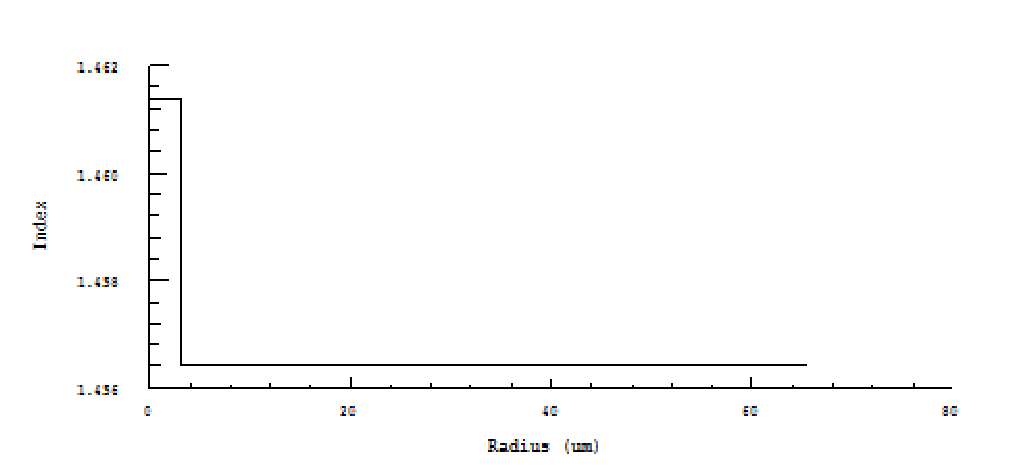
\includegraphics[scale=0.8]{fig_n.eps}\\
  \caption{Профиль показателя преломления сердцевины волокна.}\label{fig_n}
\end{figure}

\begin{figure}
  \centering
  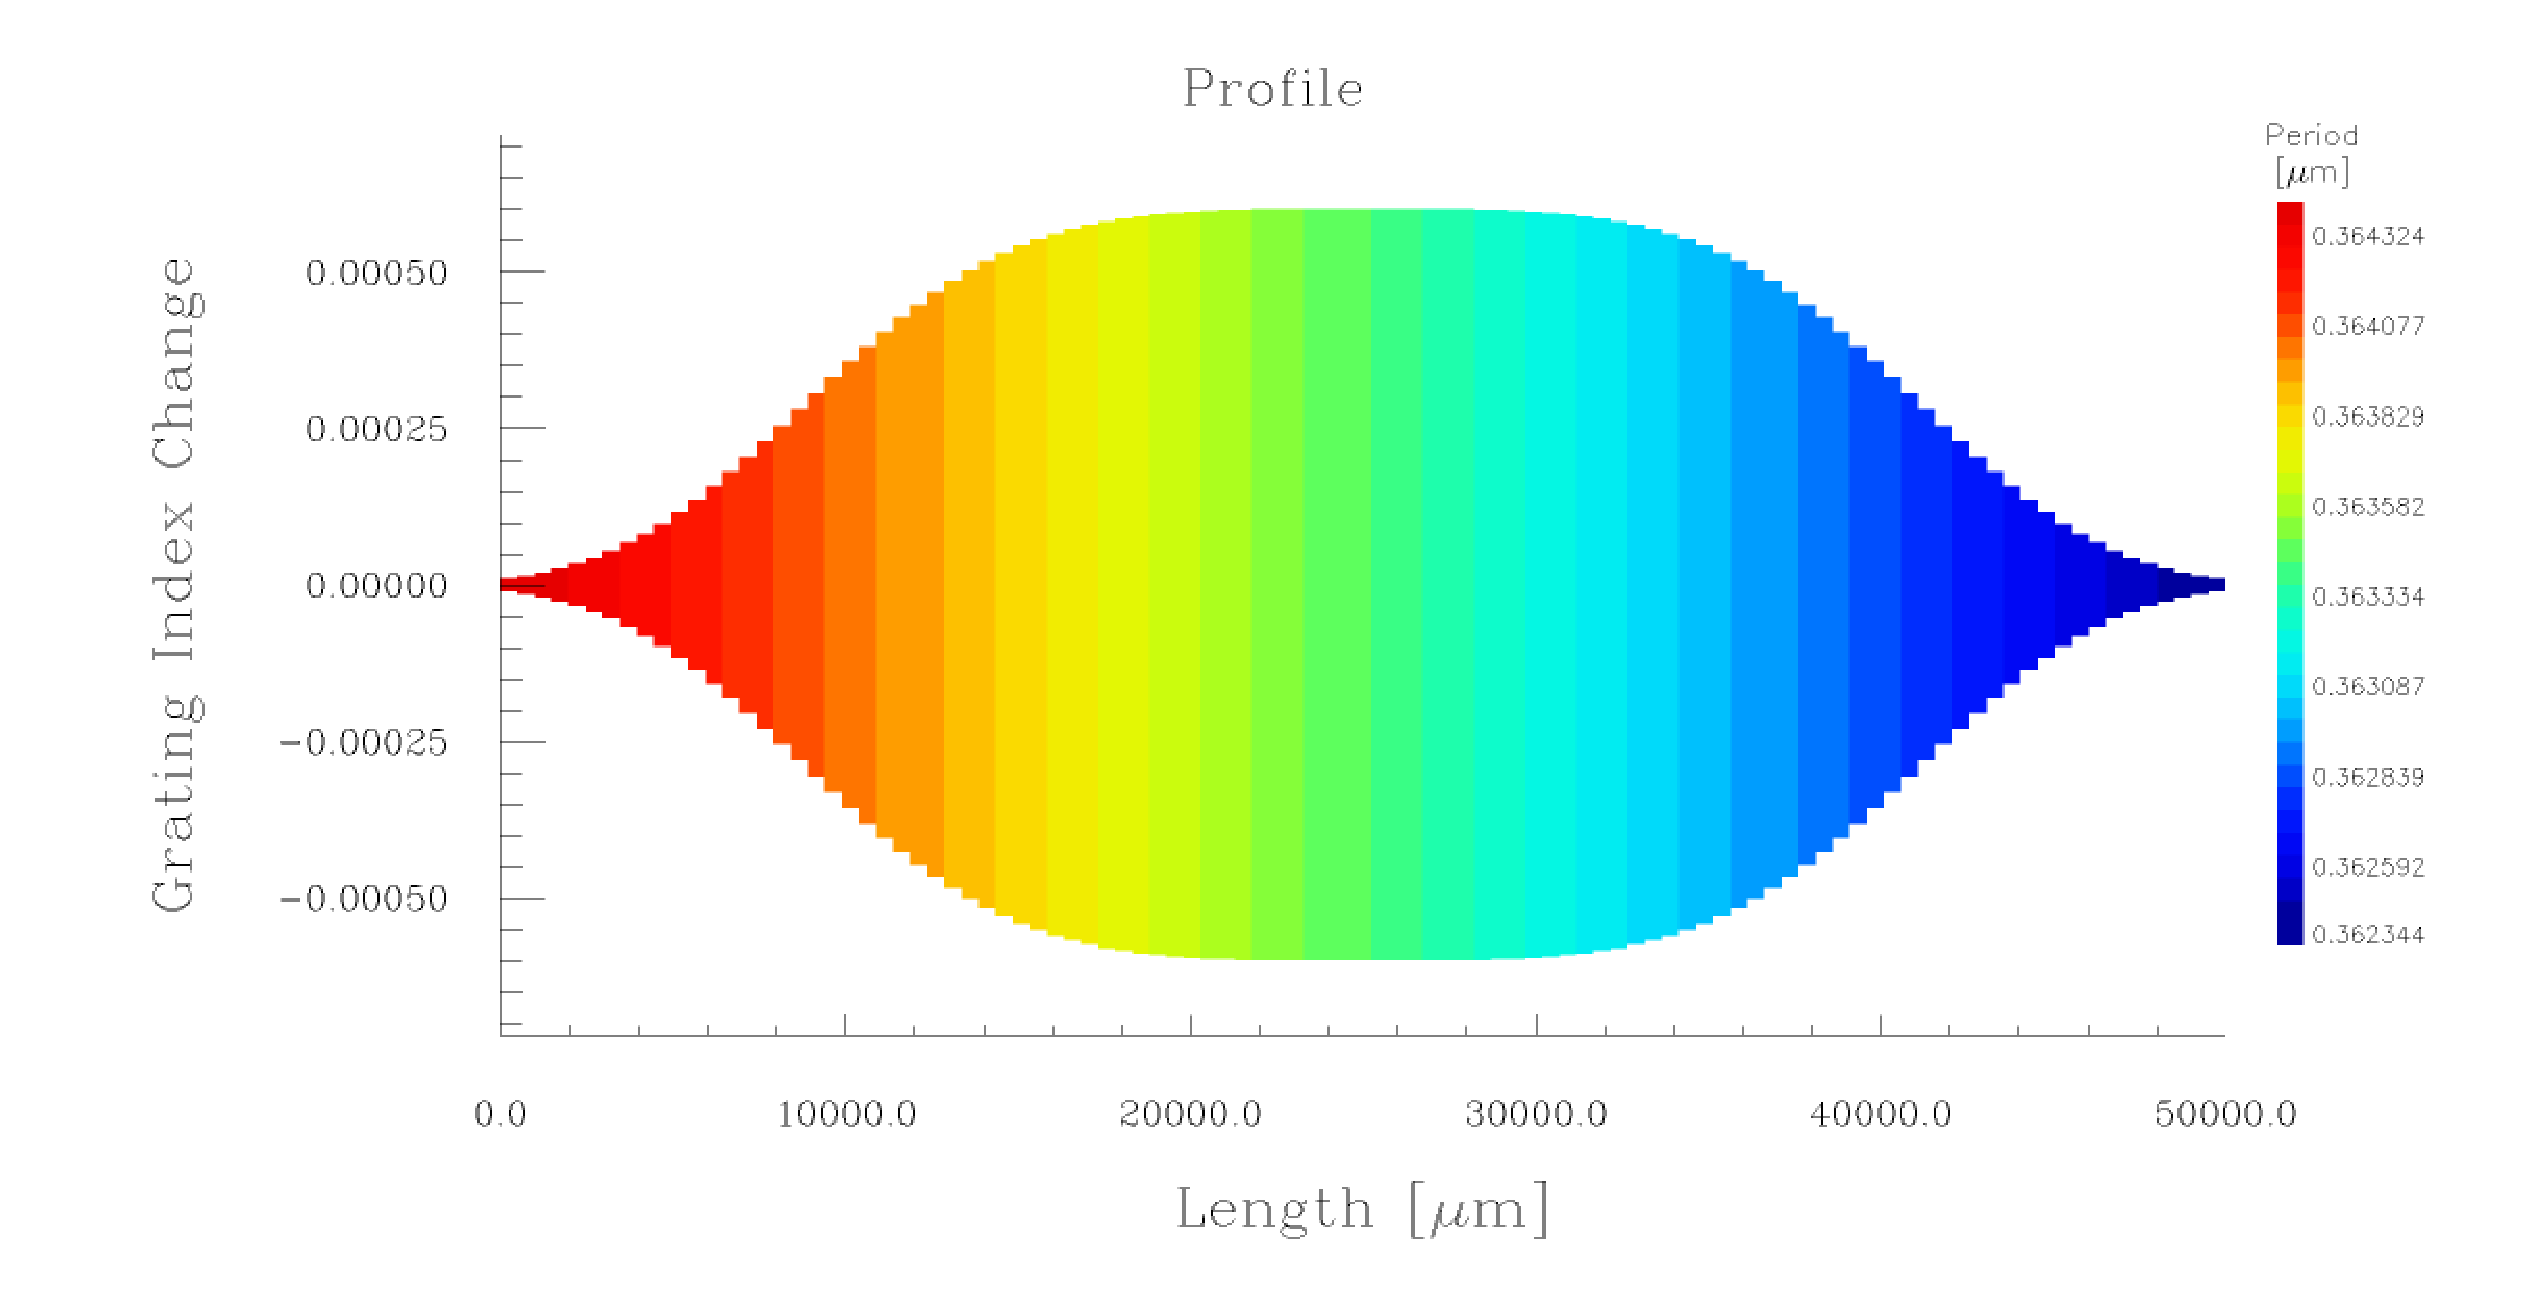
\includegraphics[scale=0.4]{fig_n_profile.eps}\\
  \caption{Профиль показателя преломления вдоль ВБР.}\label{fig_n_profile}
\end{figure}

%%%-----------------------------------------------------------------------------

\subsection{Изменение спектра ВБР при увеличении коэффициента фоточувствительности волокна}

В данном расчете с одной стороны имеет смысл проверить программу на соответствие (непротиворечие) полученных решений физическому смыслу, а с другой стороны полученные результаты важны и с чисто физической точки зрения, так как дают картину зависимости характеристик ВБР от степени фоточувствительности волокна.

На рис.~\ref{figP1} -- \ref{figP5} показаны рассчитанные спектры пропускания и отражения ВБР при различных значениях коэффициента фоточувствительности в пределах $[0,1]$. Из анализа спектров можно сделать следующие выводы:
\begin{enumerate}
\item {Наибольшая динамика изменения спектров наблюдается при малых значениях коэффициента фоточувствительности. В районе значения 0,8 степень пропускания и отражения решетки достигает своего предела и при дальнейшем увеличении коэффициента практически не изменяется.}
\item {Имеет место слабая зависимость формы и ширины (FWHM) спектра отражения от значения коэффициента фоточувствительности. Заметно изменяется только пиковое значение от -6,5 дБ при $P=$~0,2 до -0,01 дБ при $P=$~1,0.}
\item {Точка касания провала в спектре пропускания и пика в спектре отражения суть момент, когда коэффициент пропускания и отражения решетки равны 50 \%.}
\item {Следует отметить, что даже при очень слабой решетке ($\epsilon = 0$,2) спектр отражения решетки имеет полностью сформированный вид, который не изменяется при дальнейшем увеличении фоточувствительности волокна. При этом коэффициент отражения, очевидно, крайне мал.}
\end{enumerate}

\begin{figure}
  \centering
  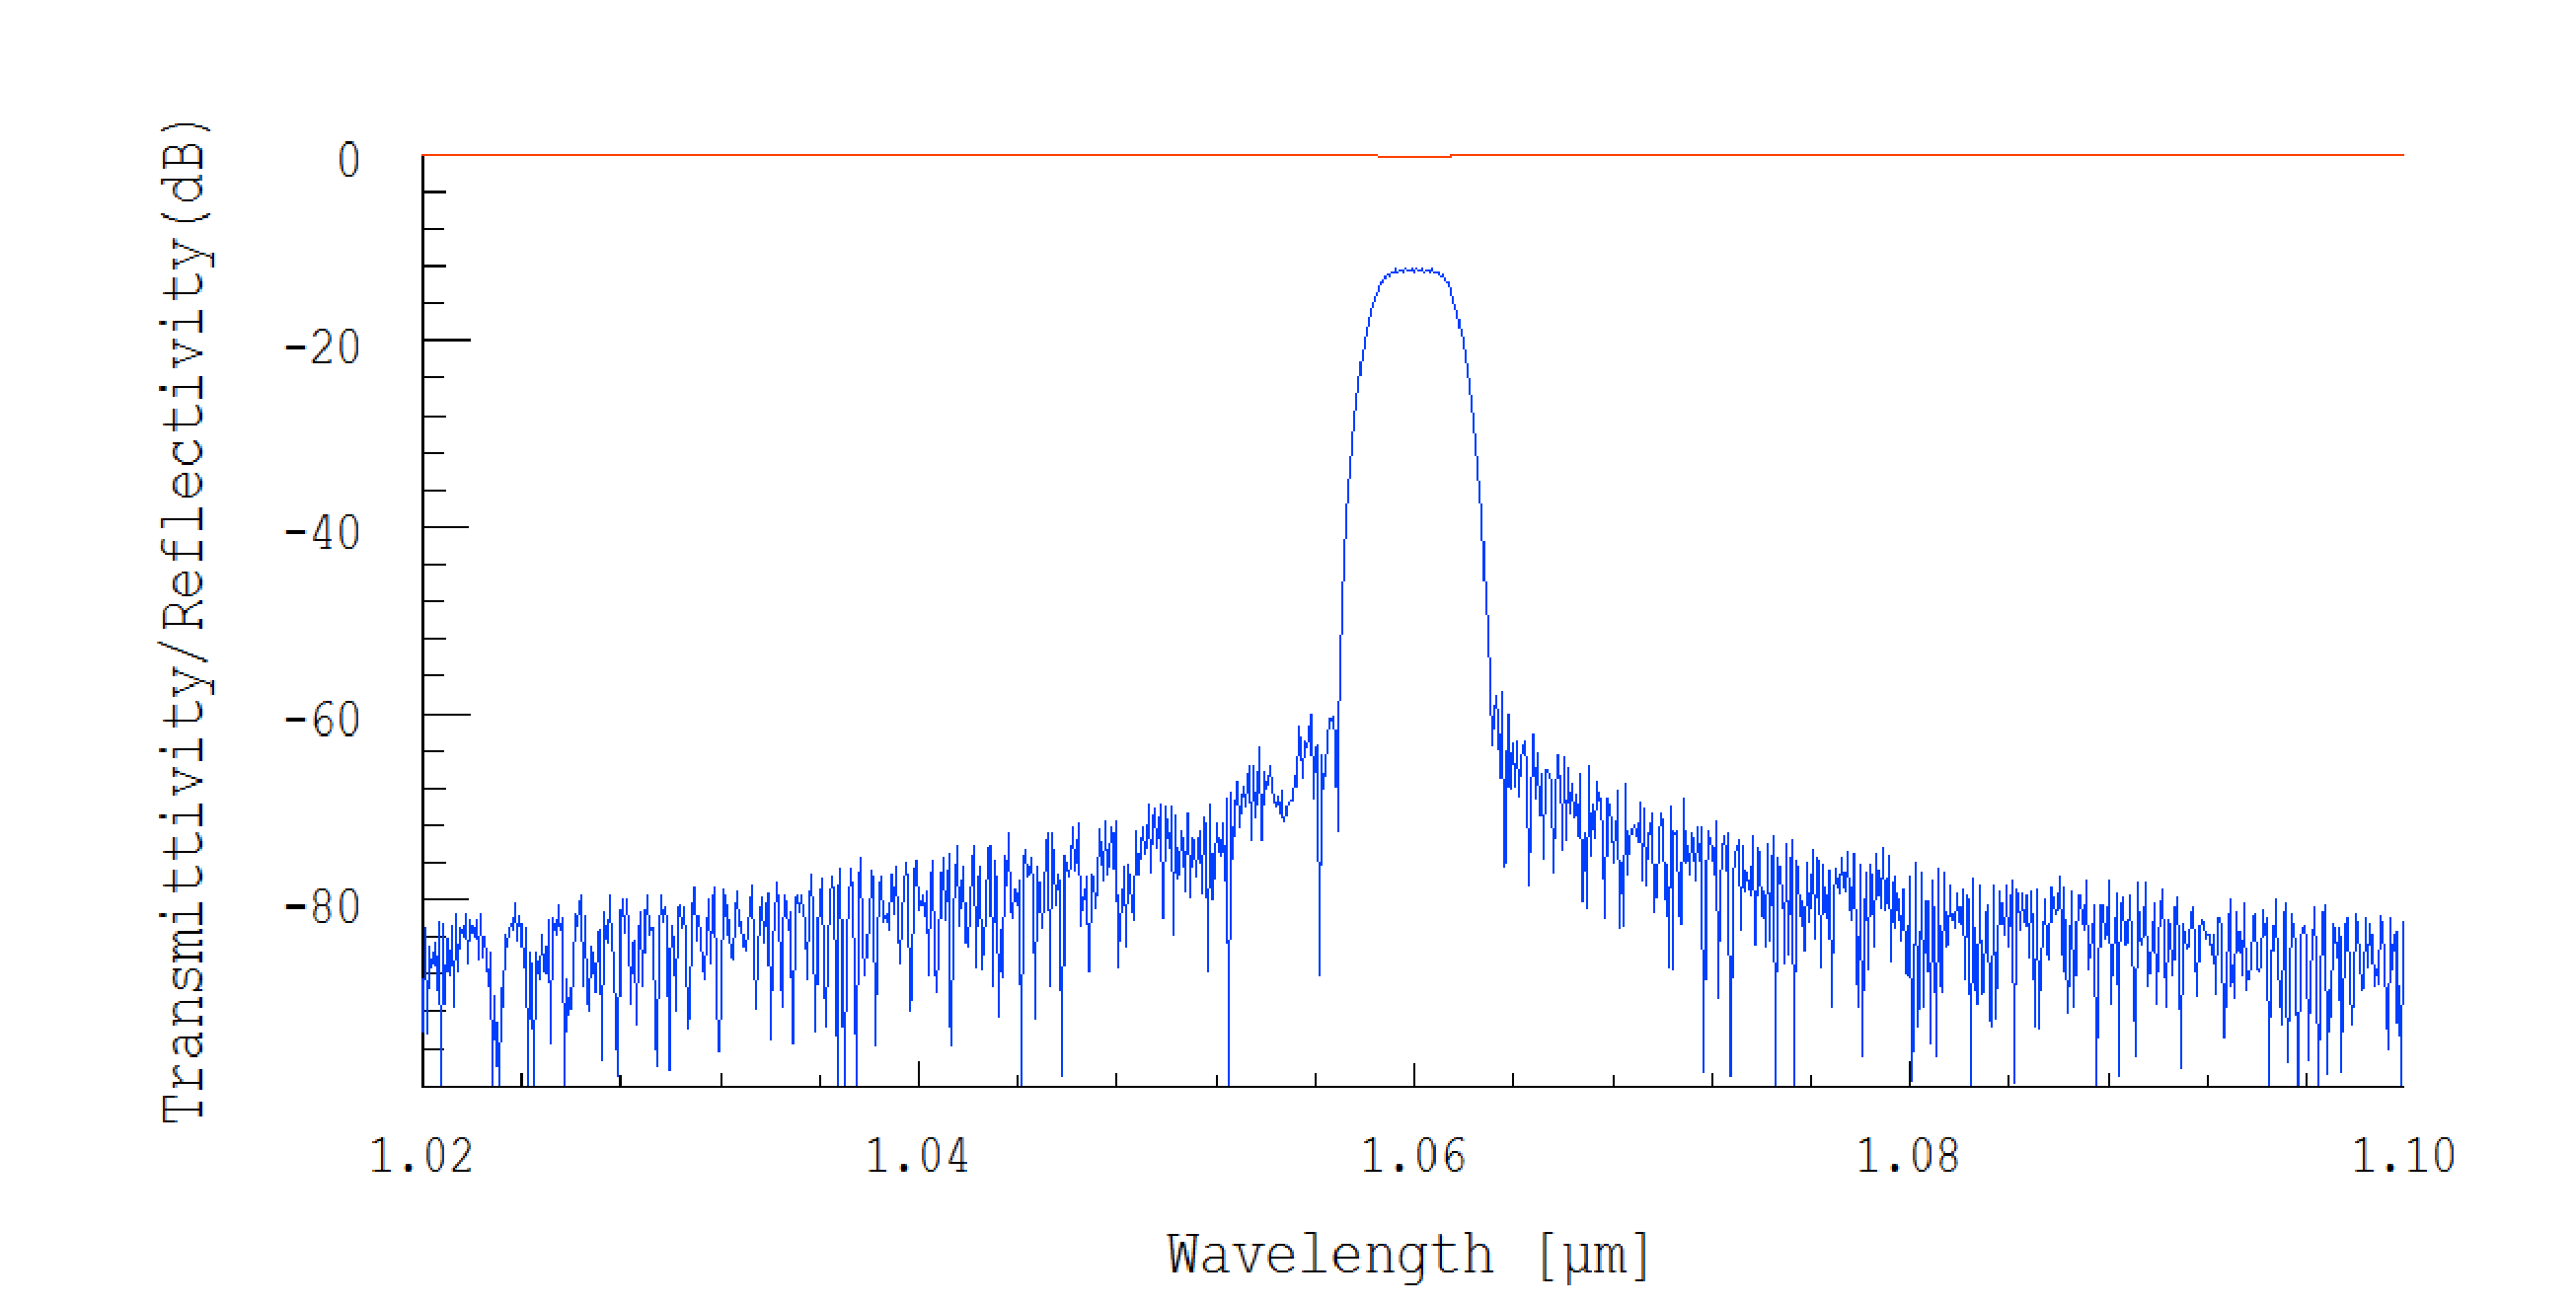
\includegraphics[scale=0.3]{fig_spec_P02.eps}\\
  \caption{Спектр пропускания и отражения ВБР при значении коэффициента фоточувствительности равного 0,2. Верхний --- пропускание, нижний --- отражение.}\label{figP1}
\end{figure}

\begin{figure}
  \centering
  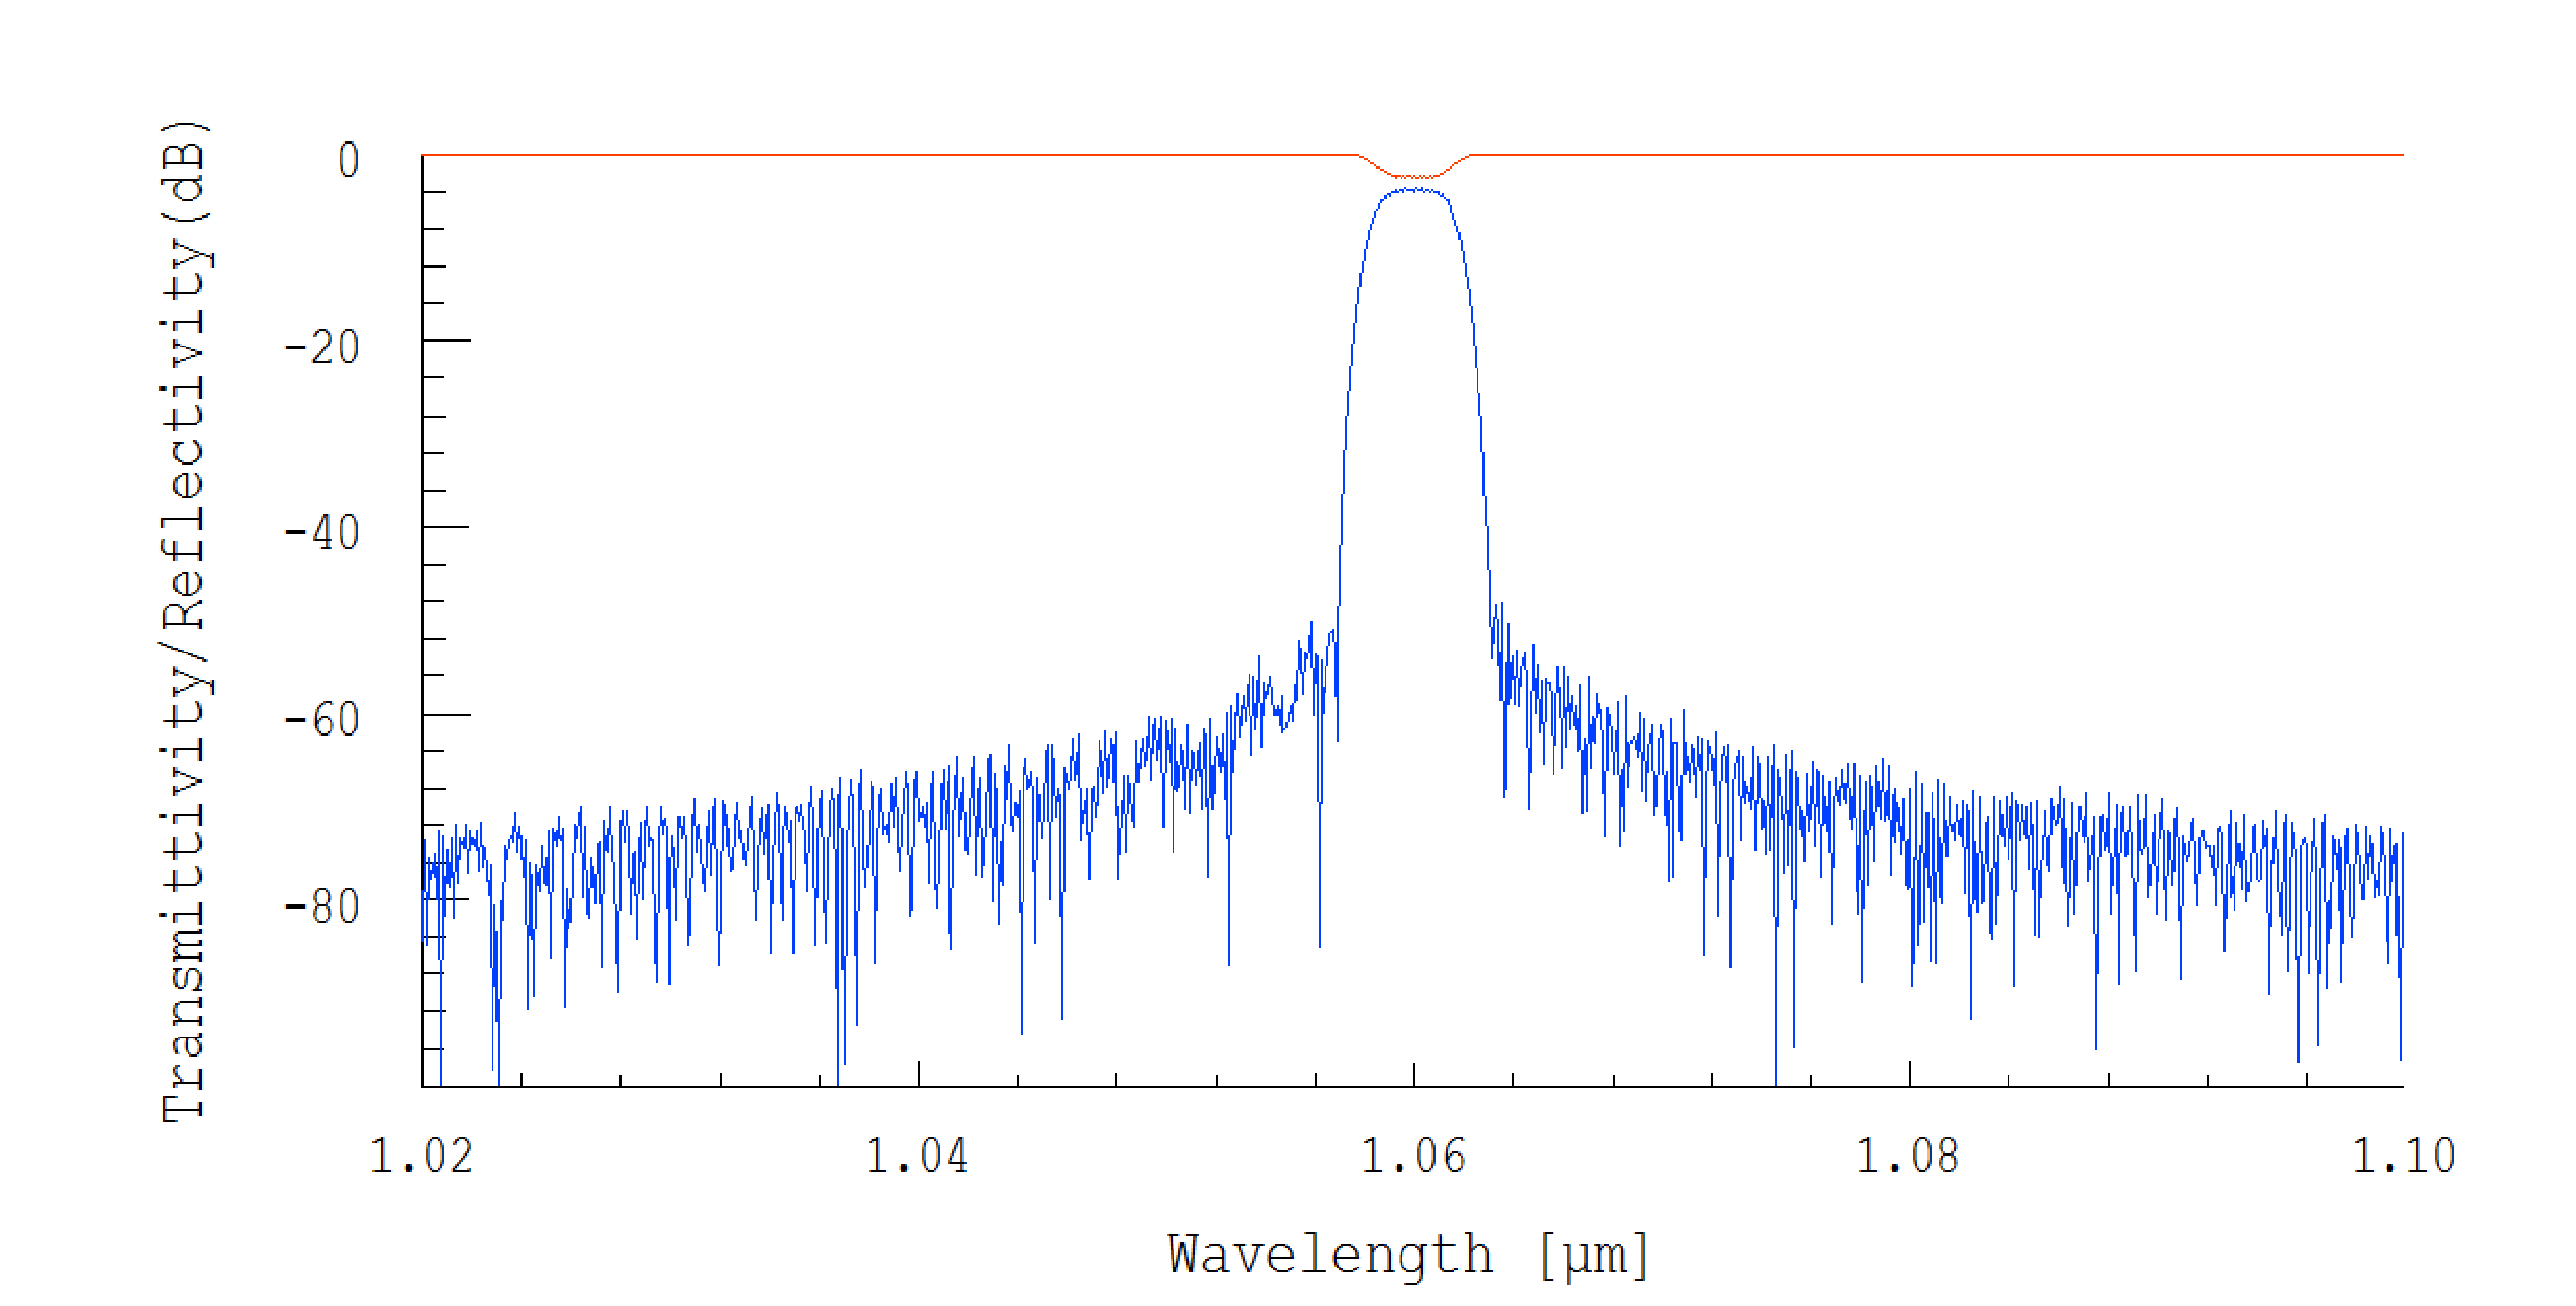
\includegraphics[scale=0.3]{fig_spec_P03.eps}\\
  \caption{Спектр пропускания и отражения ВБР при значении коэффициента фоточувствительности равного 0,3. Верхний --- пропускание, нижний --- отражение.}\label{figP2}
\end{figure}

\begin{figure}
  \centering
  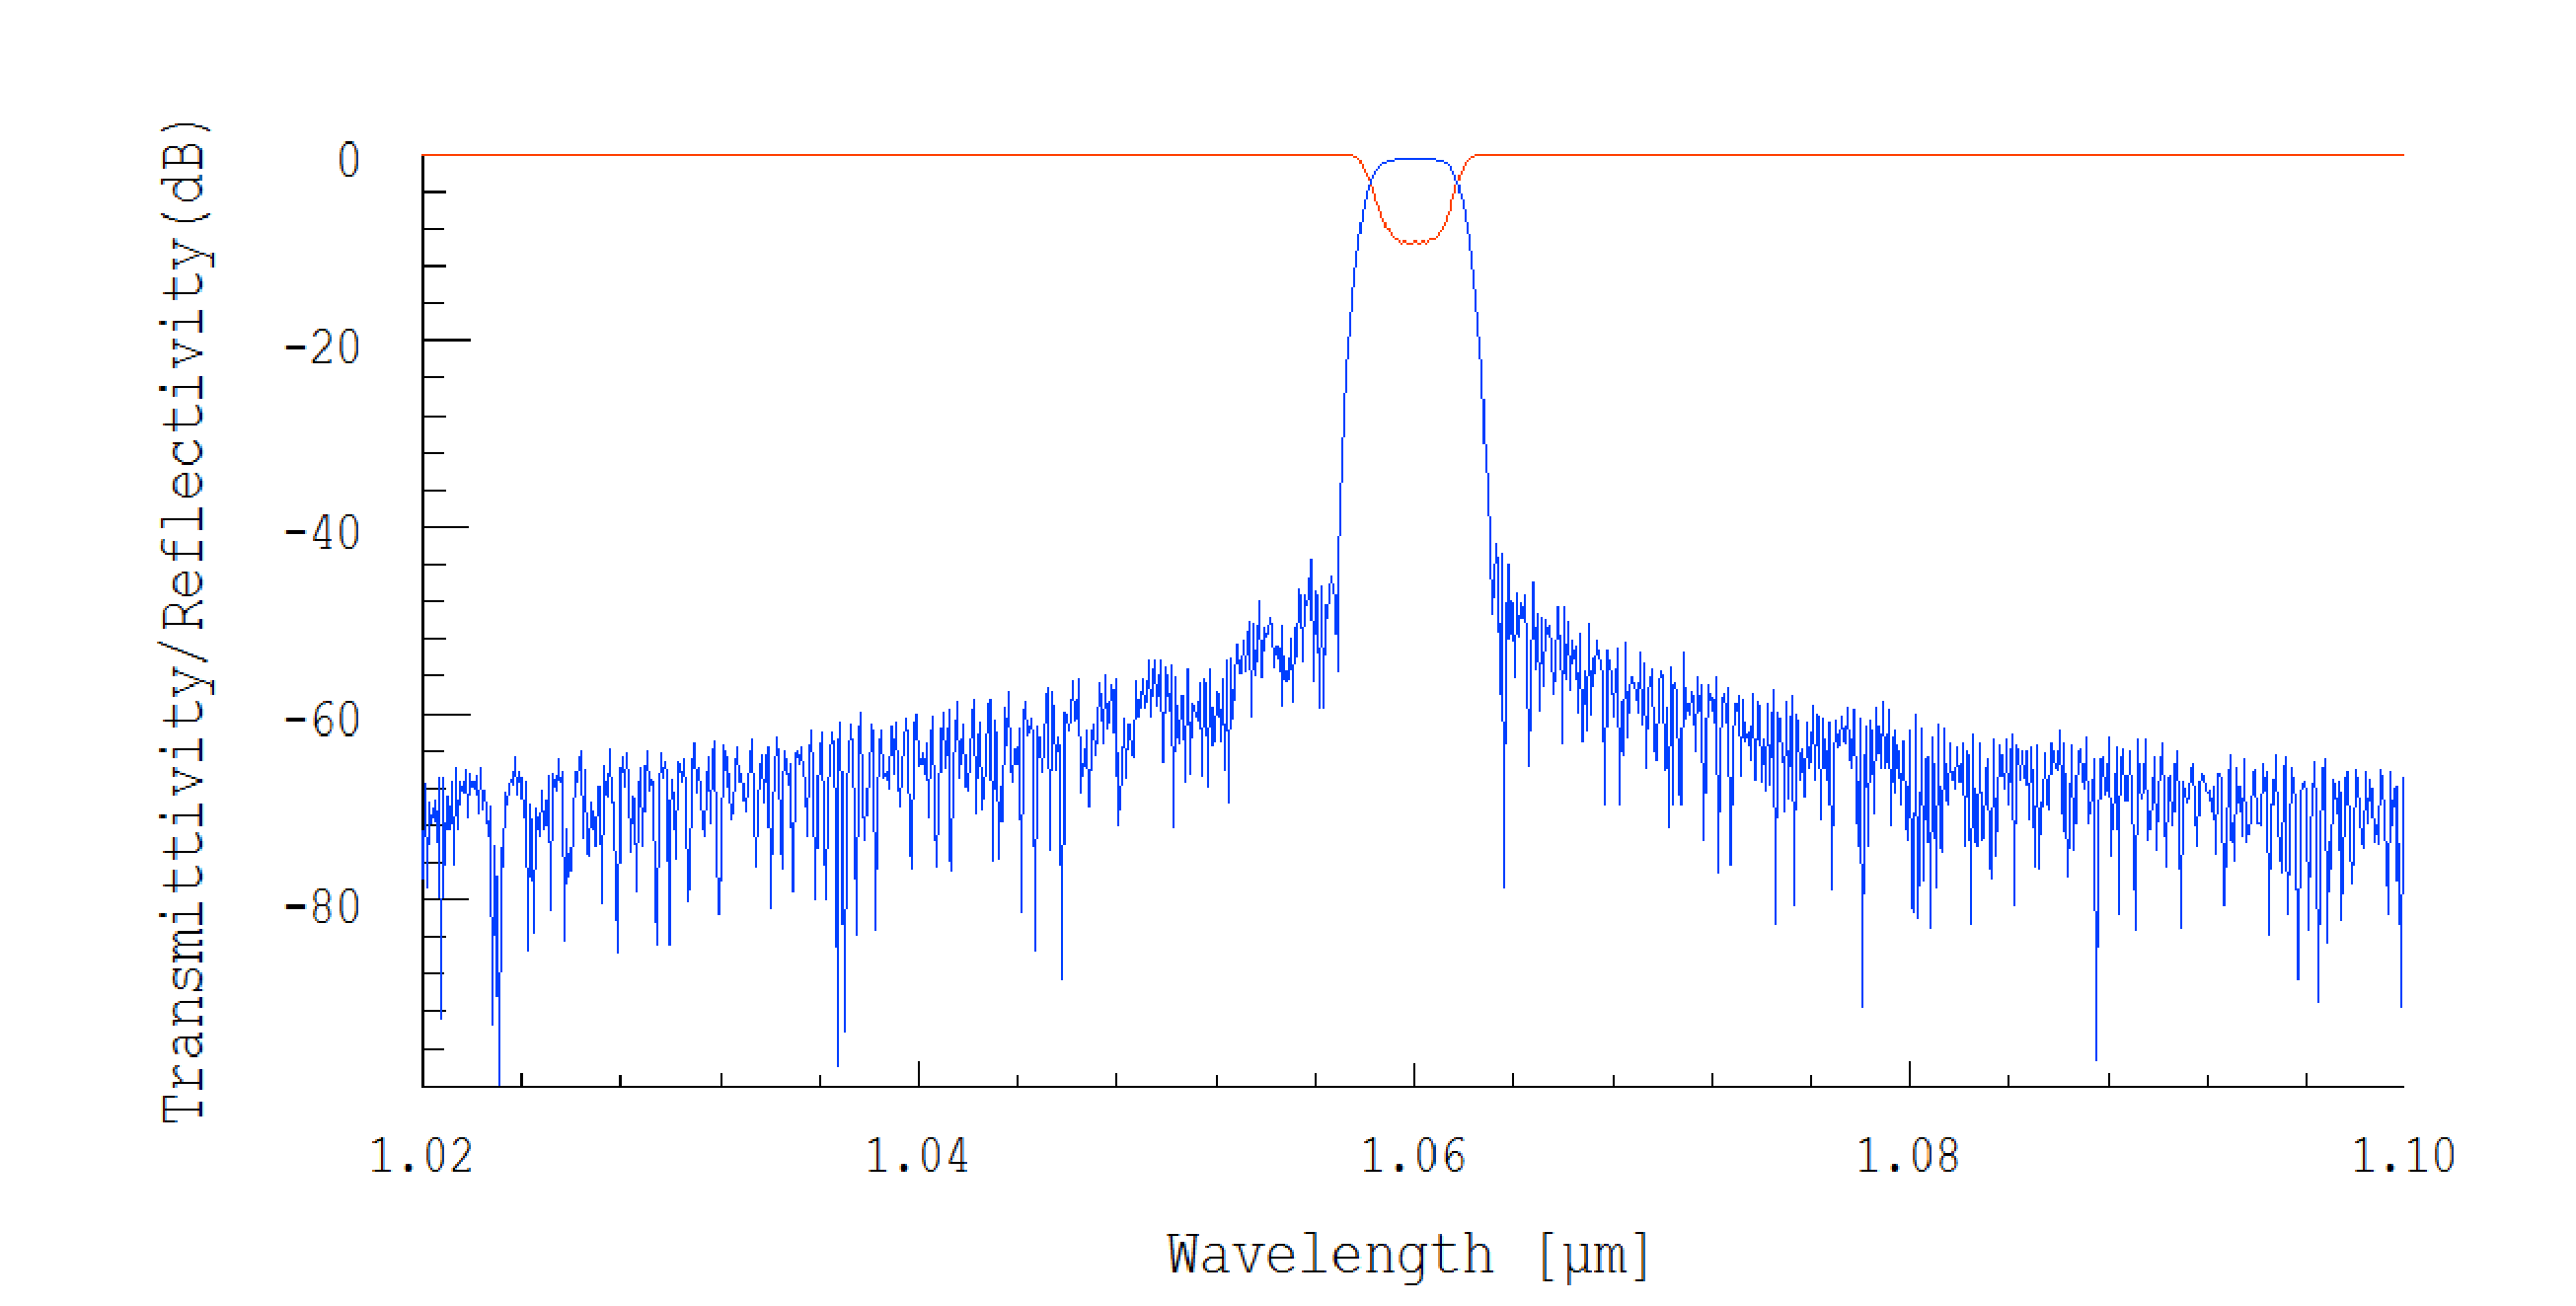
\includegraphics[scale=0.3]{fig_spec_P06.eps}\\
  \caption{Спектр пропускания и отражения ВБР при значении коэффициента фоточувствительности равного 0,6. Верхний --- пропускание, нижний --- отражение.}\label{figP3}
\end{figure}

\begin{figure}
  \centering
  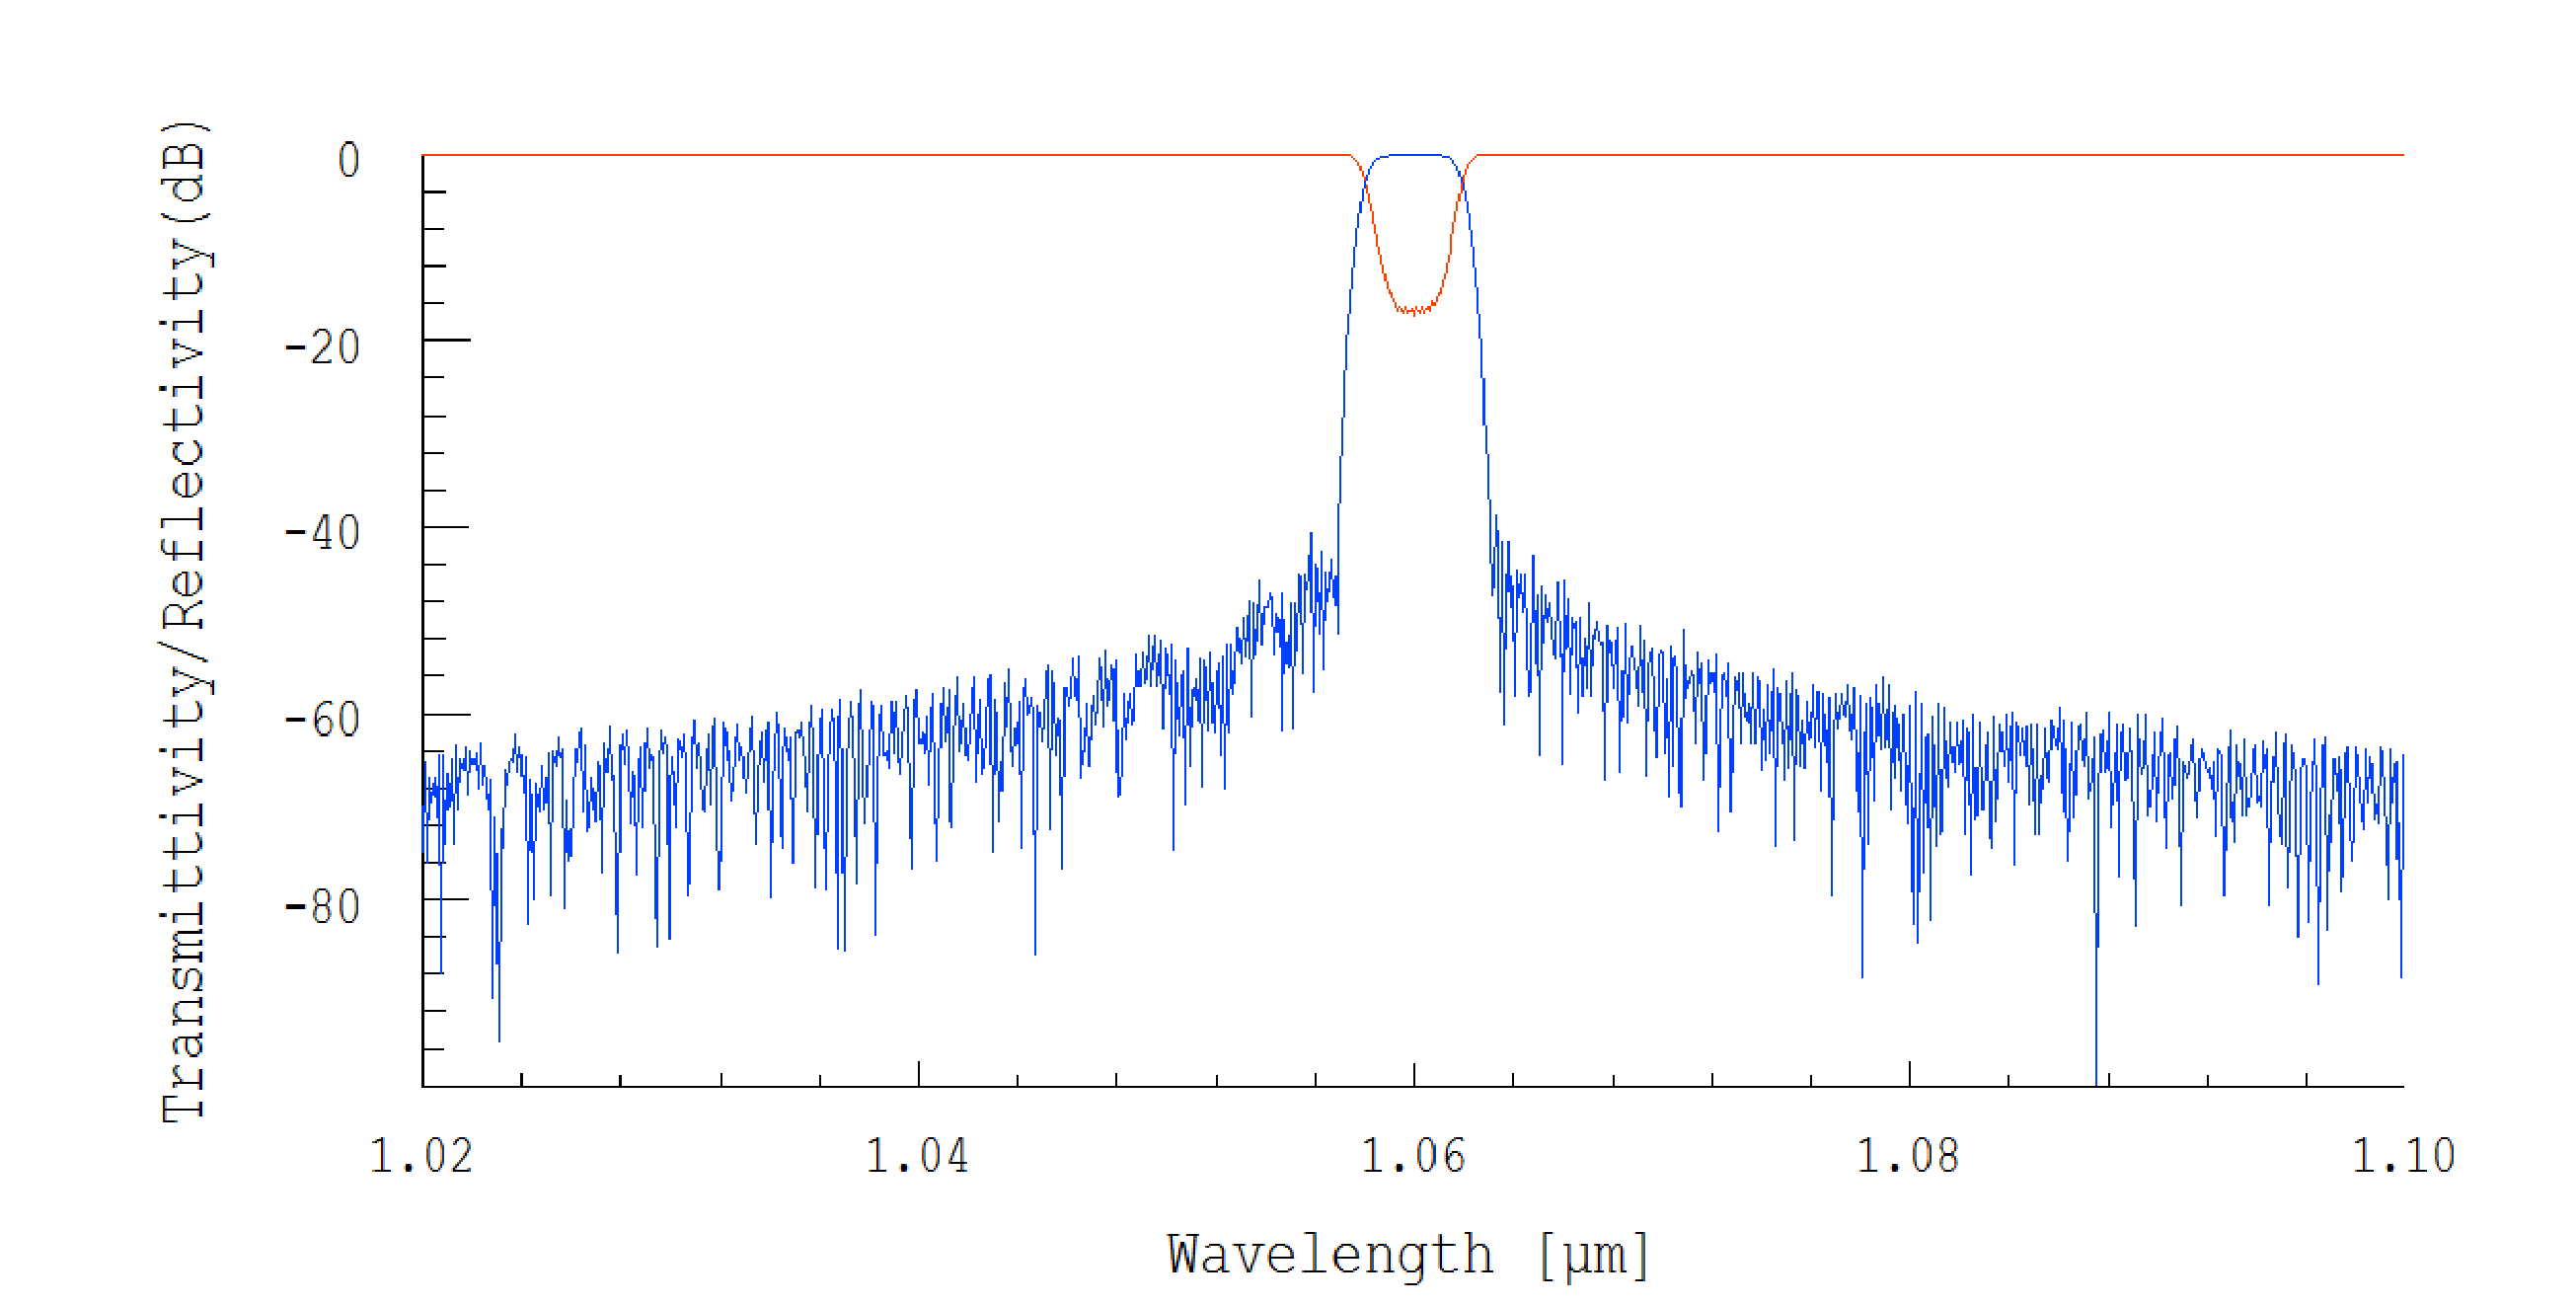
\includegraphics[scale=0.3]{fig_spec_P08.eps}\\
  \caption{Спектр пропускания и отражения ВБР при значении коэффициента фоточувствительности равного 0,8. Верхний --- пропускание, нижний --- отражение.}\label{figP4}
\end{figure}

\begin{figure}
  \centering
  \includegraphics[scale=0.3]{fig_spec_P10.eps}\\
  \caption{Спектр пропускания и отражения ВБР при значении коэффициента фоточувствительности равного 1,0. Верхний --- пропускание, нижний --- отражение.}\label{figP5}
\end{figure}

Из рис. \ref{figP6} -- \ref{figP10} видно, что имеет место очевидная связь между фоточувствительностью волокна и коэффициентом отражения решетки. Чем выше фоточувствительность (при фиксированном значении дозы облучения), тем выше коэффициент отражения. Иными словами, хорошие ВБР зеркала получаются из <<сильных>> решеток (т.~е. с высоким наведенным ПП).

\begin{figure}
  \centering
  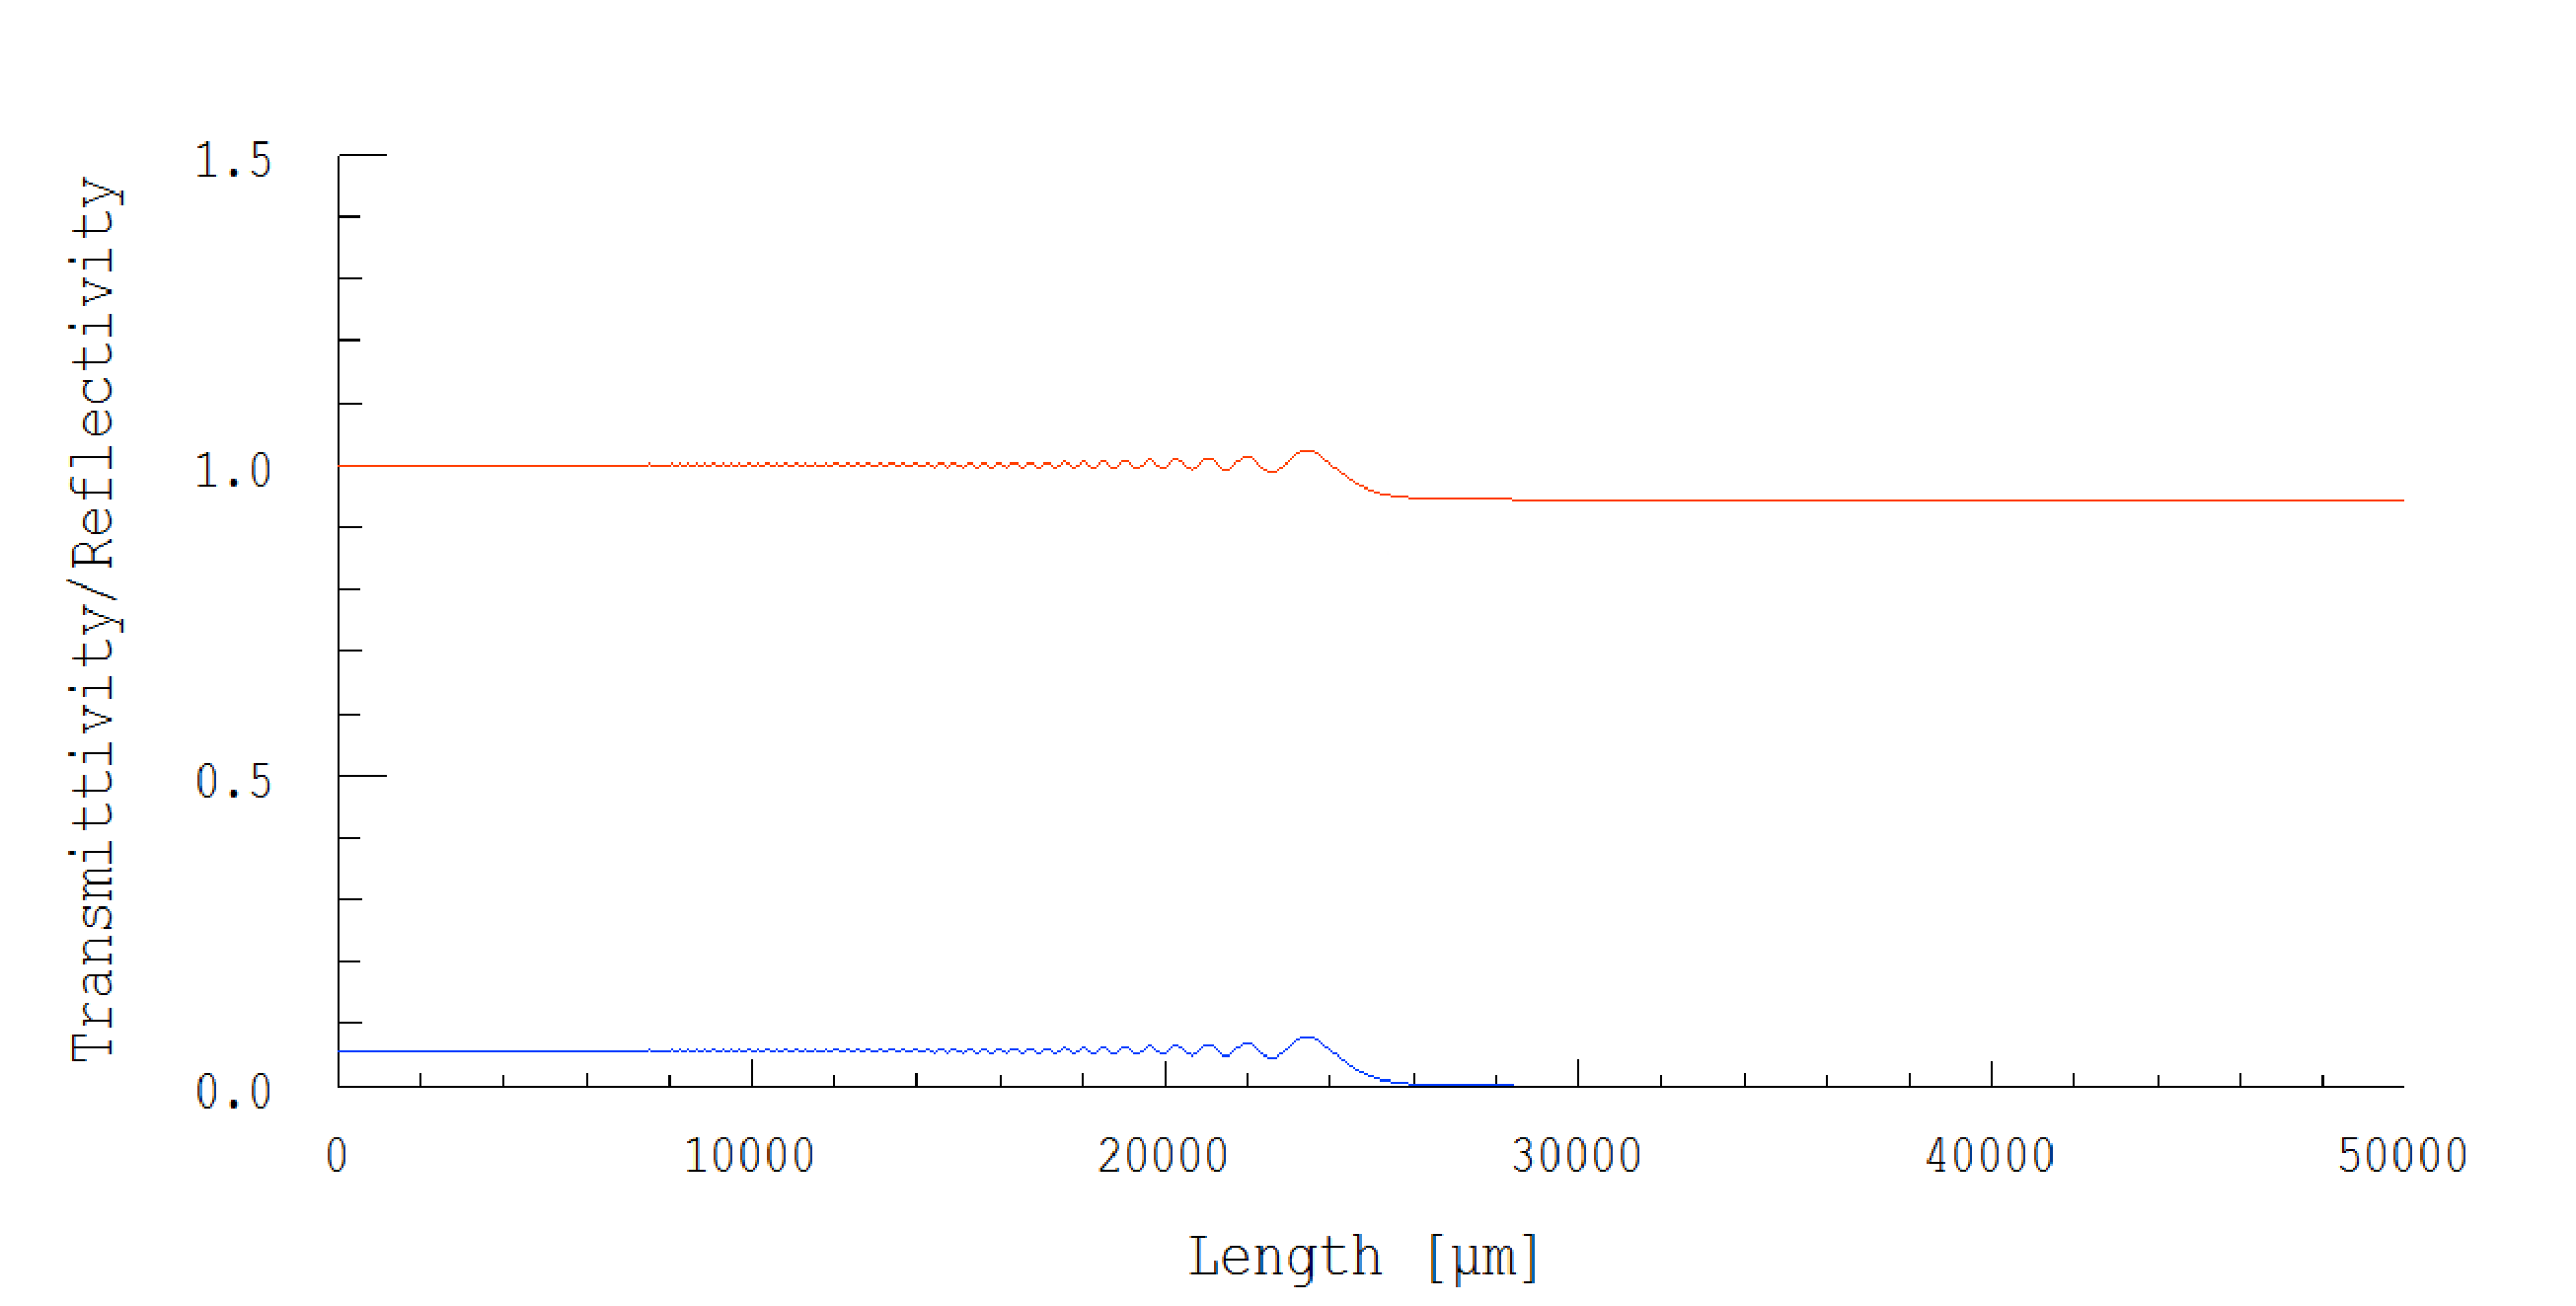
\includegraphics[scale=0.3]{fig_power_P02.eps}\\
  \caption{График отражения и пропускания ВБР в расчёте на единицу мощности проходящего излучения при значении коэффициента фоточувствительности равного 0,2. Верхний --- пропускание, нижний --- отражение.}\label{figP6}
\end{figure}

\begin{figure}
  \centering
  \includegraphics[scale=0.3]{fig_power_P03.eps}\\
  \caption{График отражения и пропускания ВБР в расчёте на единицу мощности проходящего излучения при значении коэффициента фоточувствительности равного 0,3. Верхний --- пропускание, нижний --- отражение.}\label{figP7}
\end{figure}

\begin{figure}
  \centering
  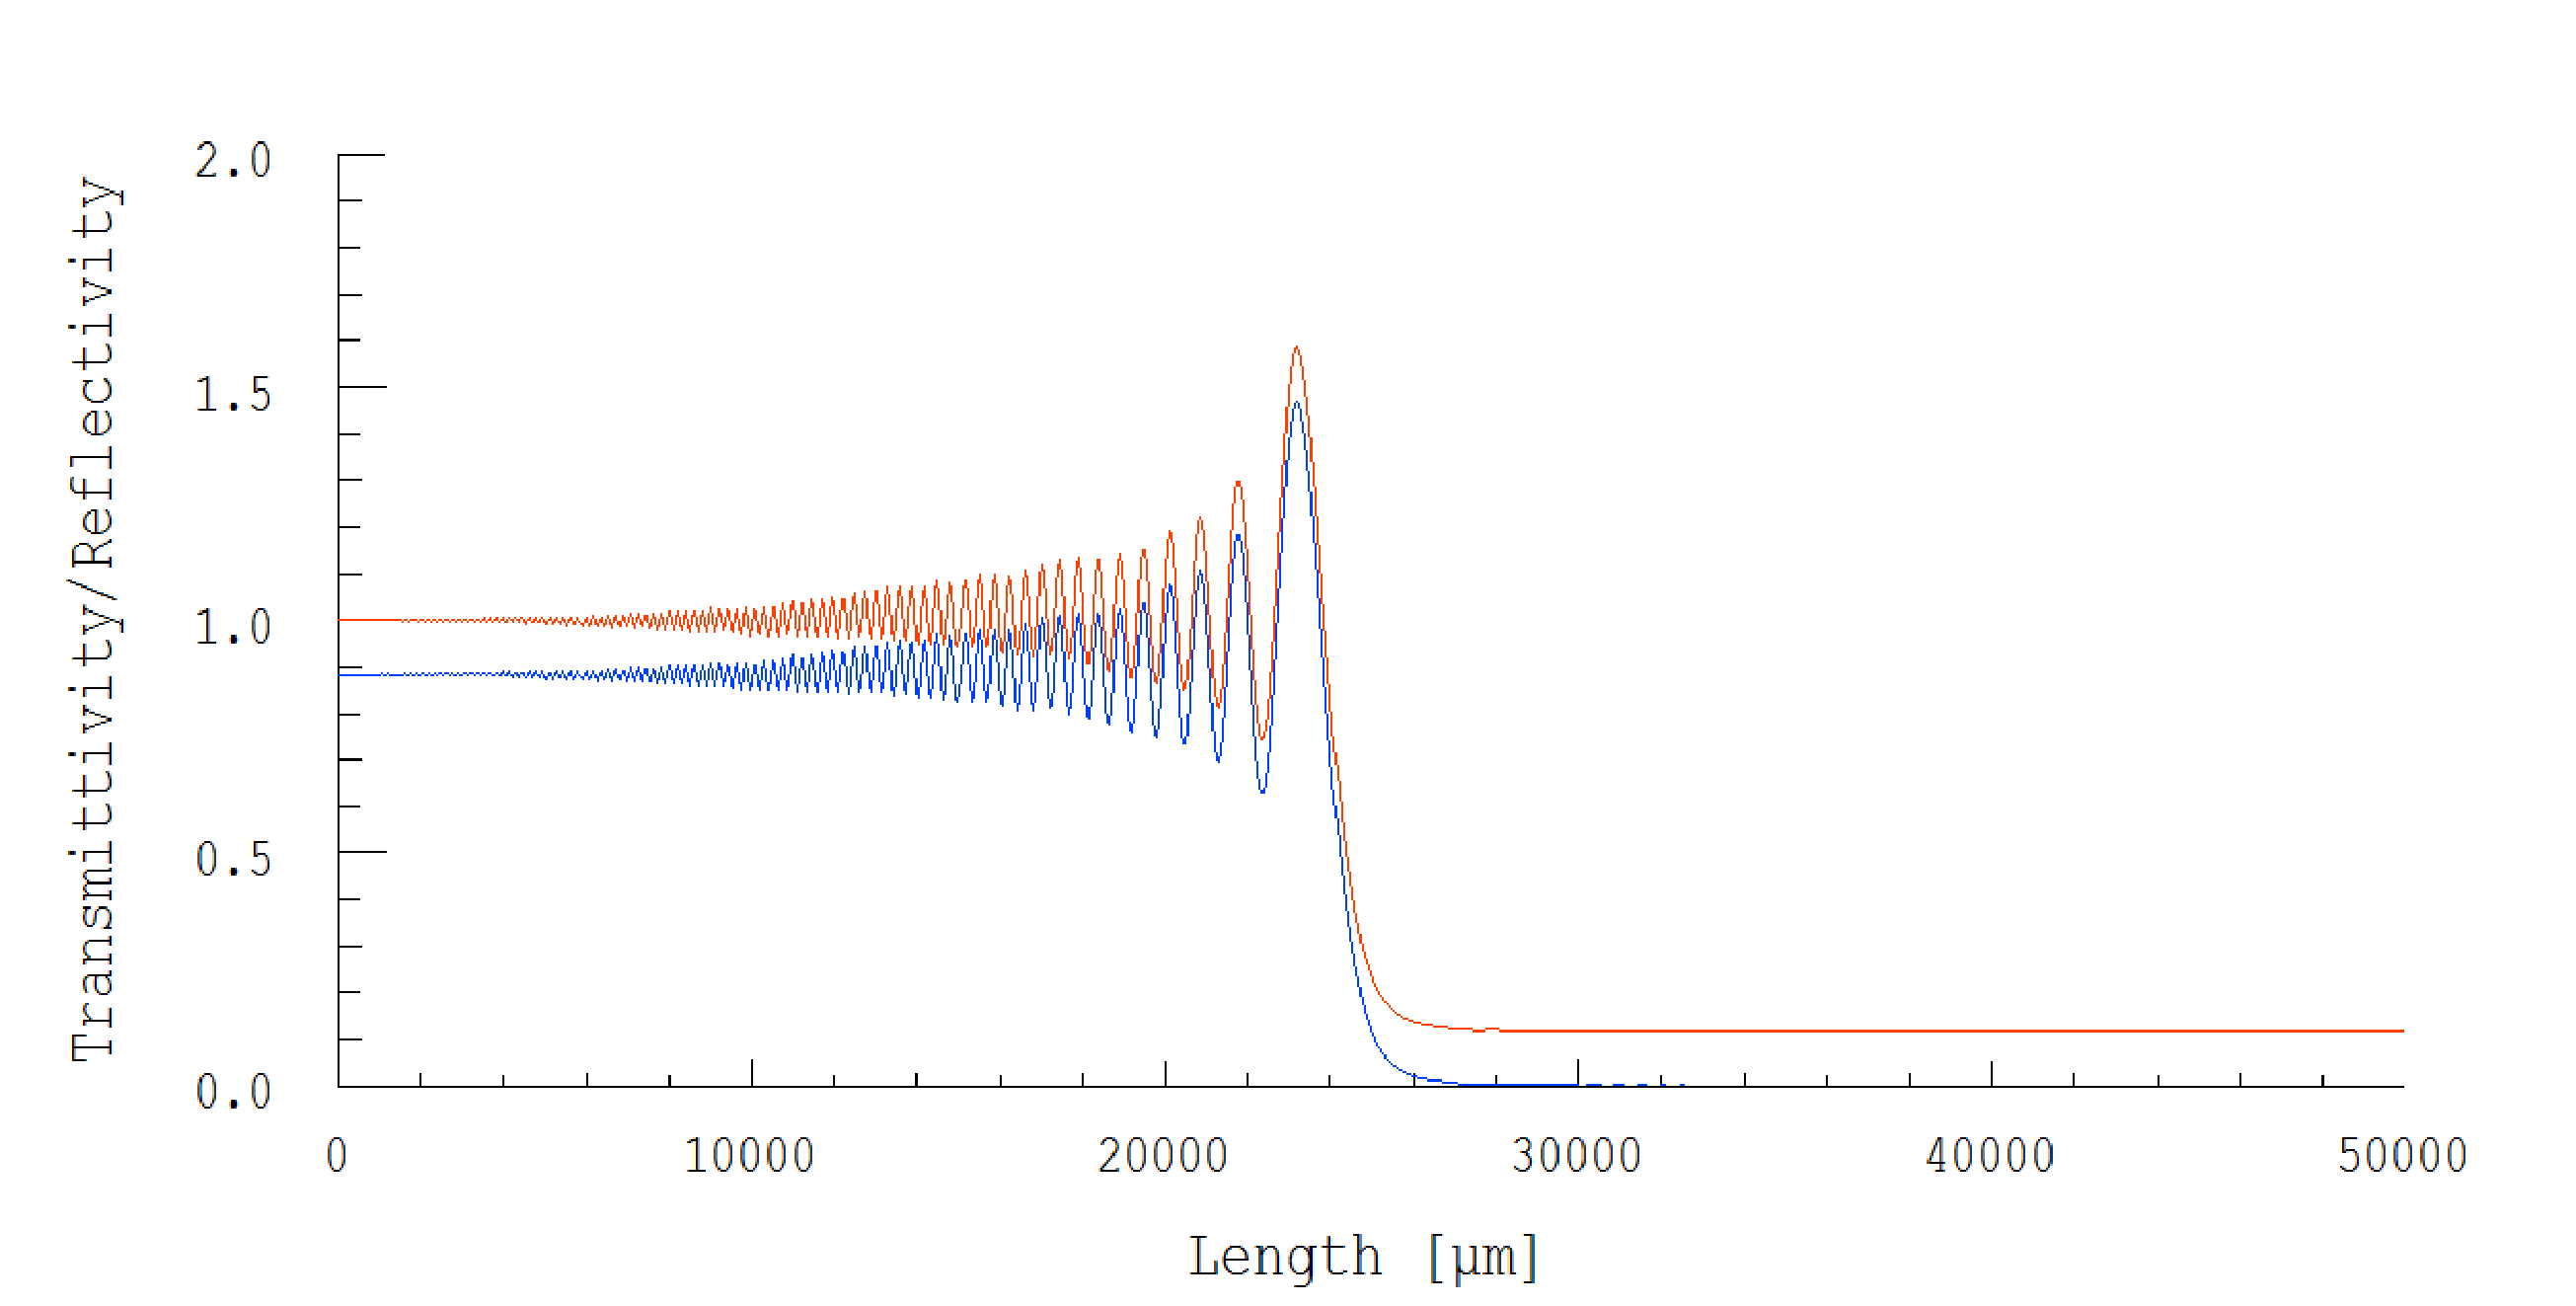
\includegraphics[scale=0.3]{fig_power_P06.eps}\\
  \caption{График отражения и пропускания ВБР в расчёте на единицу мощности проходящего излучения при значении коэффициента фоточувствительности равного 0,6. Верхний --- пропускание, нижний --- отражение.}\label{figP8}
\end{figure}

\begin{figure}
  \centering
  \includegraphics[scale=0.3]{fig_power_P08.eps}\\
  \caption{График отражения и пропускания ВБР в расчёте на единицу мощности проходящего излучения при значении коэффициента фоточувствительности равного 0,8. Верхний --- пропускание, нижний --- отражение.}\label{figP9}
\end{figure}

\begin{figure}
  \centering
  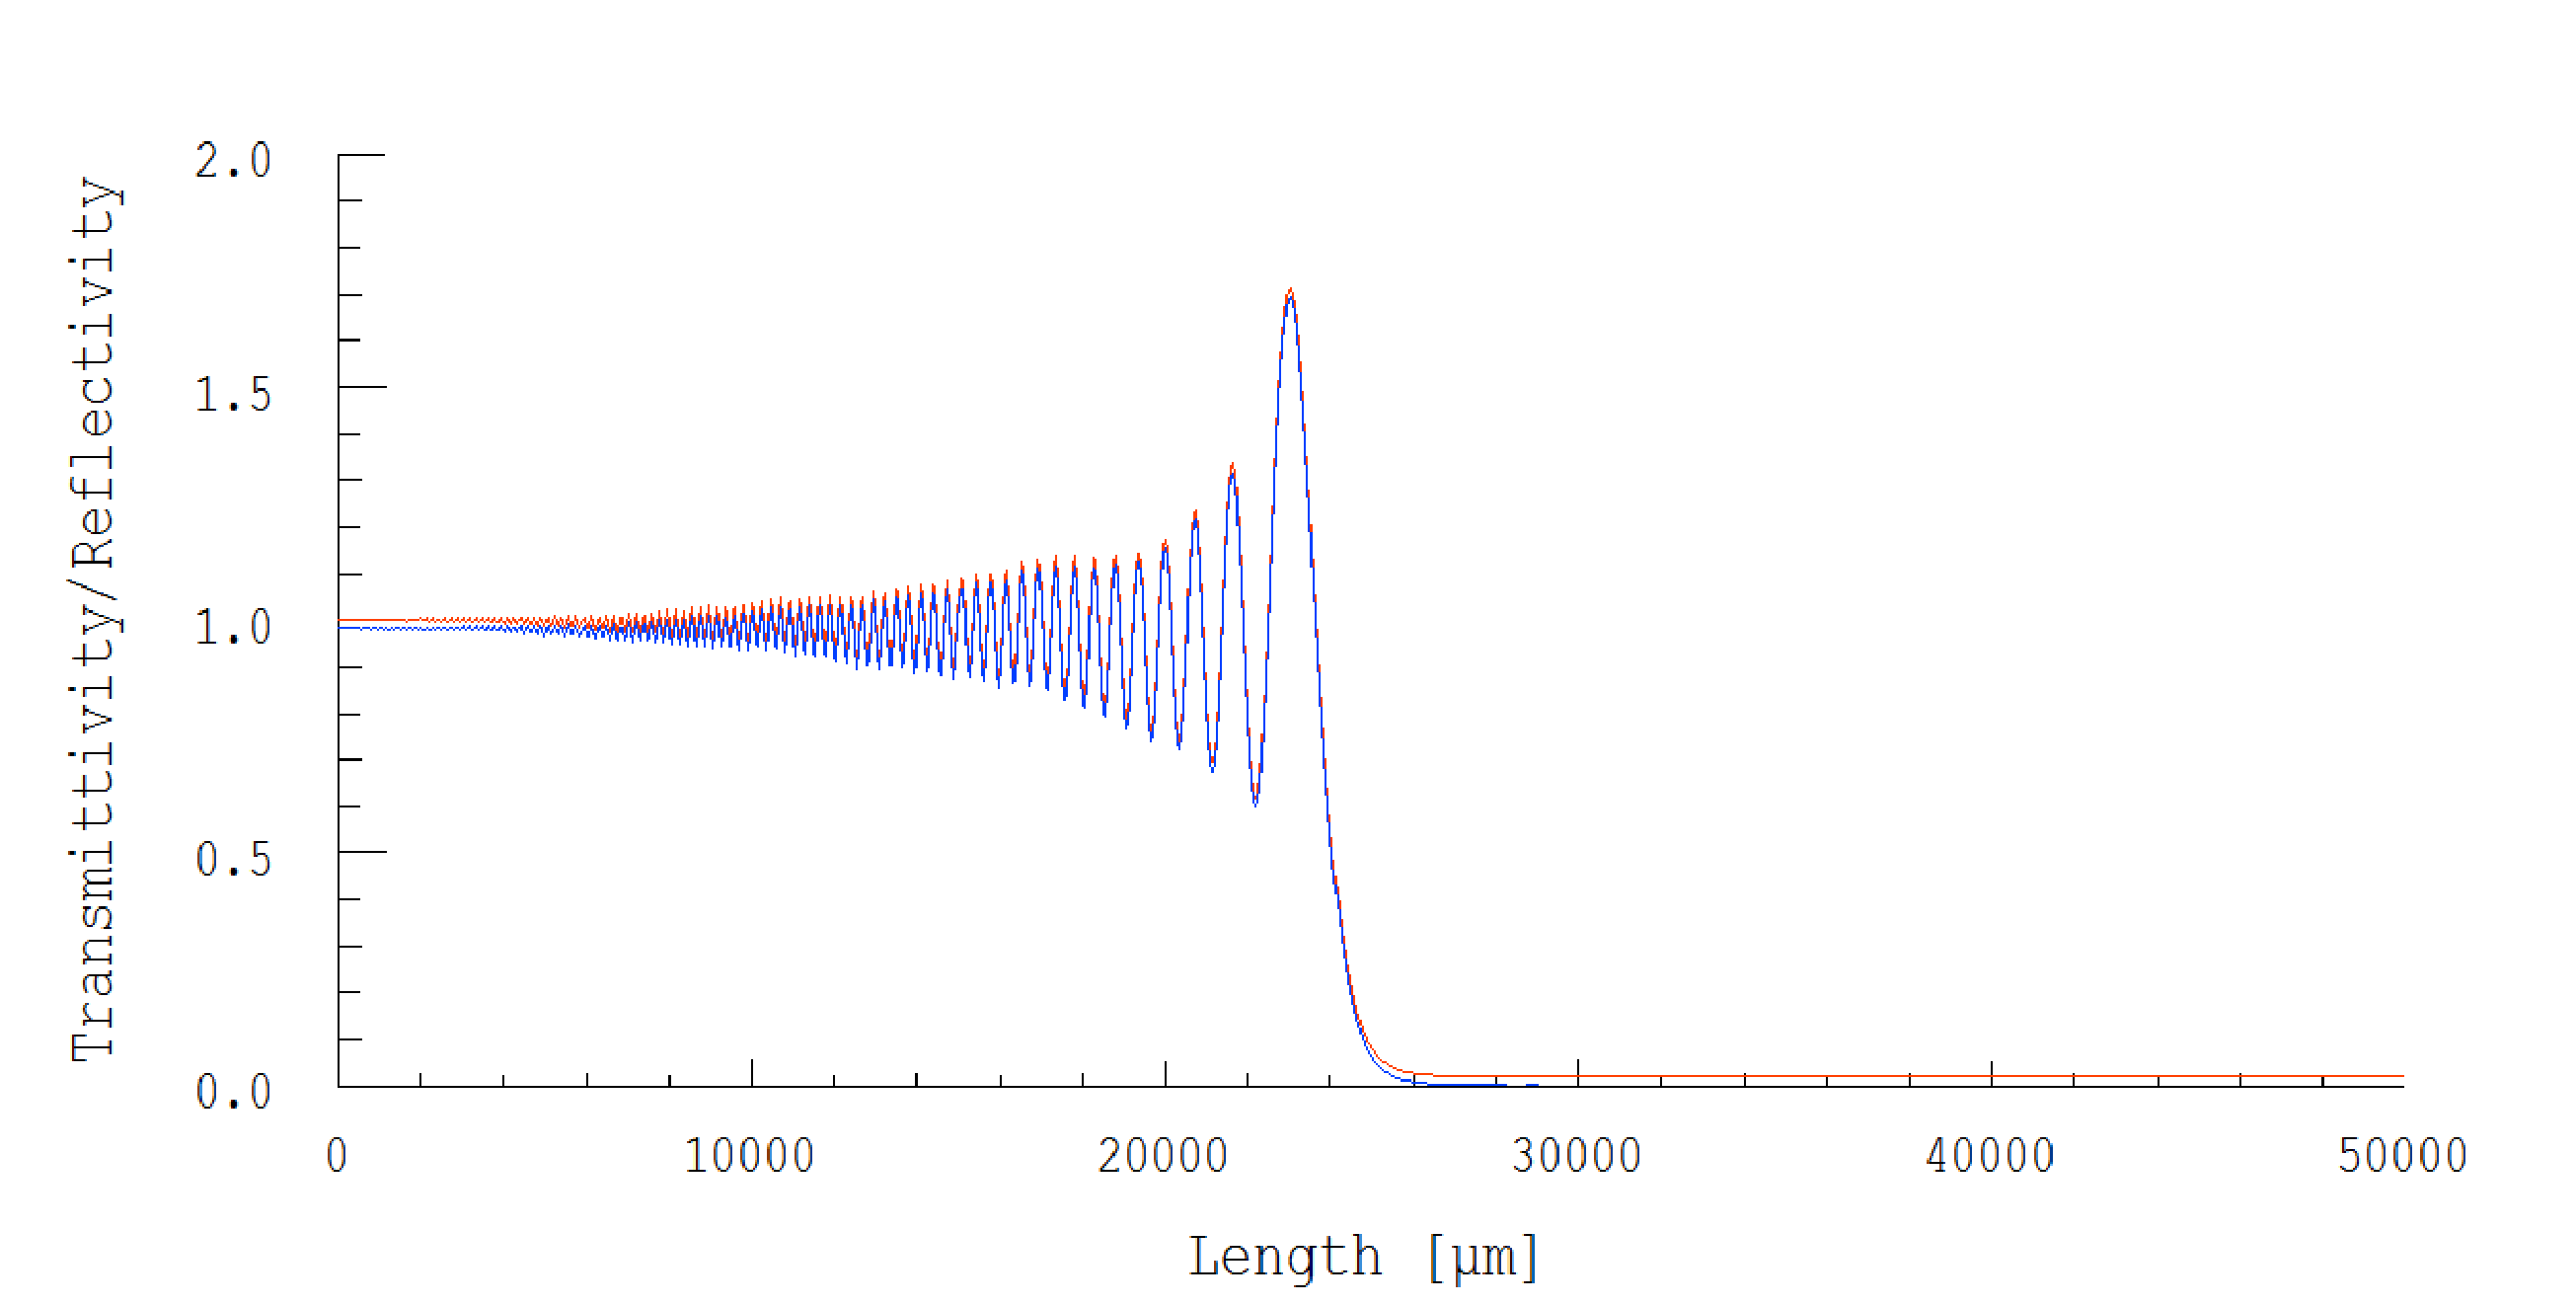
\includegraphics[scale=0.3]{fig_power_P10.eps}\\
  \caption{График отражения и пропускания ВБР в расчёте на единицу мощности проходящего излучения при значении коэффициента фоточувствительности равного 1,0. Верхний --- пропускание, нижний --- отражение.}\label{figP10}
\end{figure}

%%%-----------------------------------------------------------------------------

\subsection{Профили фоточувствительности сердцевины волокна}

Для моделирования волокна с неоднородным распределением фоточувствительности в поперечном сечении волокна были взяты произвольные функциональные зависимости гипотетического значения фоточувствительности от значения $x \in [ 0,R ]$.

Постоянный:
\begin{equation} \label{eq2.1}
    \epsilon(x)=const.
\end{equation}

Линейный:
\begin{equation} \label{eq2.2}
    \epsilon(x)=\epsilon(0)+y \cdot\frac{\epsilon(R)-\epsilon(0)}{R}.
\end{equation}

Параболический:
\begin{equation} \label{eq2.3}
    \epsilon(x)=[\epsilon(R)-\epsilon(0)]\cdot\left(\frac{y}{R}\right)^2+\epsilon(0).
\end{equation}

Экспоненциальный:
\begin{equation} \label{eq2.4}
    \epsilon(x)=[\epsilon(0)-\epsilon(R)]\cdot\frac{e}{e-1}\cdot\exp\left(-\frac{y}{R}\right)+\frac{e\cdot\epsilon(R)-\epsilon(0)}{e-1}.
\end{equation}

Гауссовый:
\begin{equation} \label{eq2.5}
    \epsilon(x)=n_{max}\cdot\exp\left\lbrace-ln2\cdot\left[\frac{2\cdot(y-y_0)^2}{h\cdot R}\right]\right\rbrace.
\end{equation}

Альфа-пик:
\begin{equation} \label{eq2.6}
    \epsilon(x)=n_{max}\cdot\sqrt{1-2\Delta\cdot\left(\frac{y}{R}\right)^\alpha}.
\end{equation}

Альфа-провал:
\begin{equation} \label{eq2.7}
    \epsilon(x)=n_{max}\cdot\sqrt{1-2\Delta\cdot\left(1-\frac{y}{R}\right)^\alpha}.
\end{equation}

Графики всех использованных функций приведены на рисунке~\ref{fig_profiles}, где мы использовали следующие значения констант: $\epsilon(0)=1, \epsilon(R)=0, R=3, \alpha=2, \Delta=\:$0,5, $h=10$.

\begin{figure}
\centering
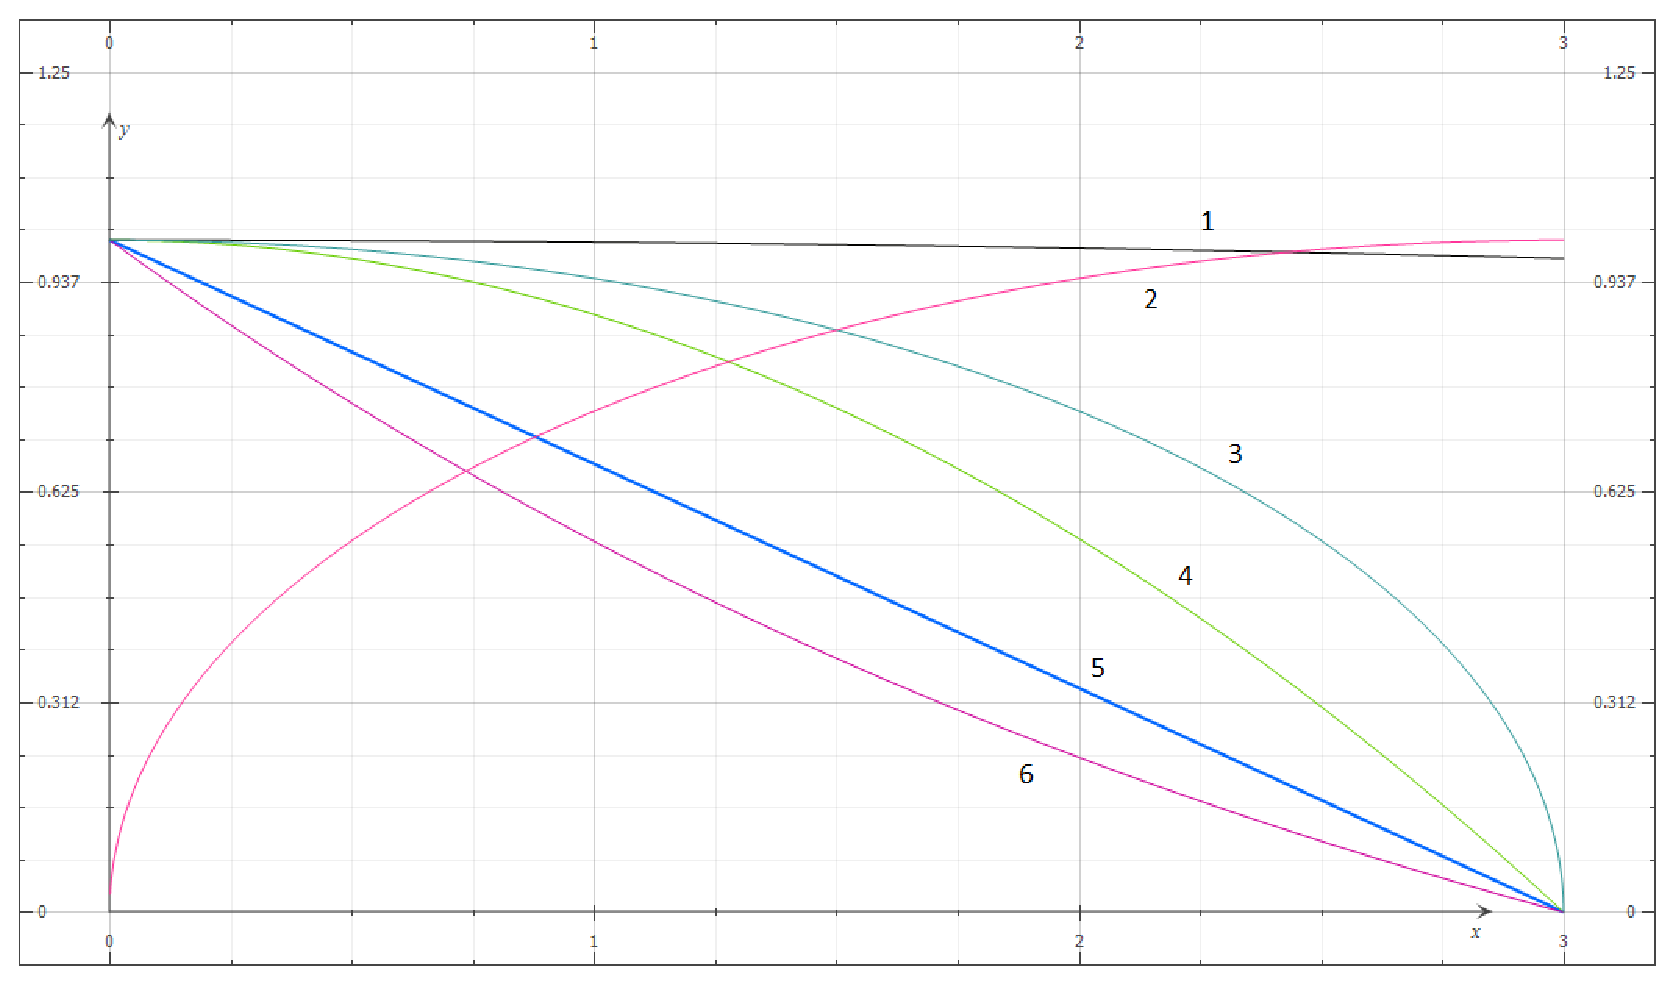
\includegraphics[scale=0.5]{fig_profiles.eps}
\caption{График профилей фоточувствительности: 1 --- гауссовый, 2 --- альфа-провал, 3 --- альфа-пик, 4 --- параболический, 5 --- линейный, 6 --- экспоненциальный.}\label{fig_profiles}
\end{figure}

Важно отметить (см. рис.~\ref{fig_length_5} -- \ref{fig_length_20}), что теоретически, даже при достаточно низкой фоточувствительности материала оптоволокна (на котором записывается решетка) при увеличении длины записываемой ВБР (например, беря фазовые маски большего размера) мы можем достичь очень высокой отражательной способности. В показанном расчете при коэффициенте фоточувствительности равном 0,3, увеличив длину ВБР с 5 мм до 2 см, мы увеличили отражательную способность ВБР с 40 \% до 86 \%.

\begin{figure}
  \centering
  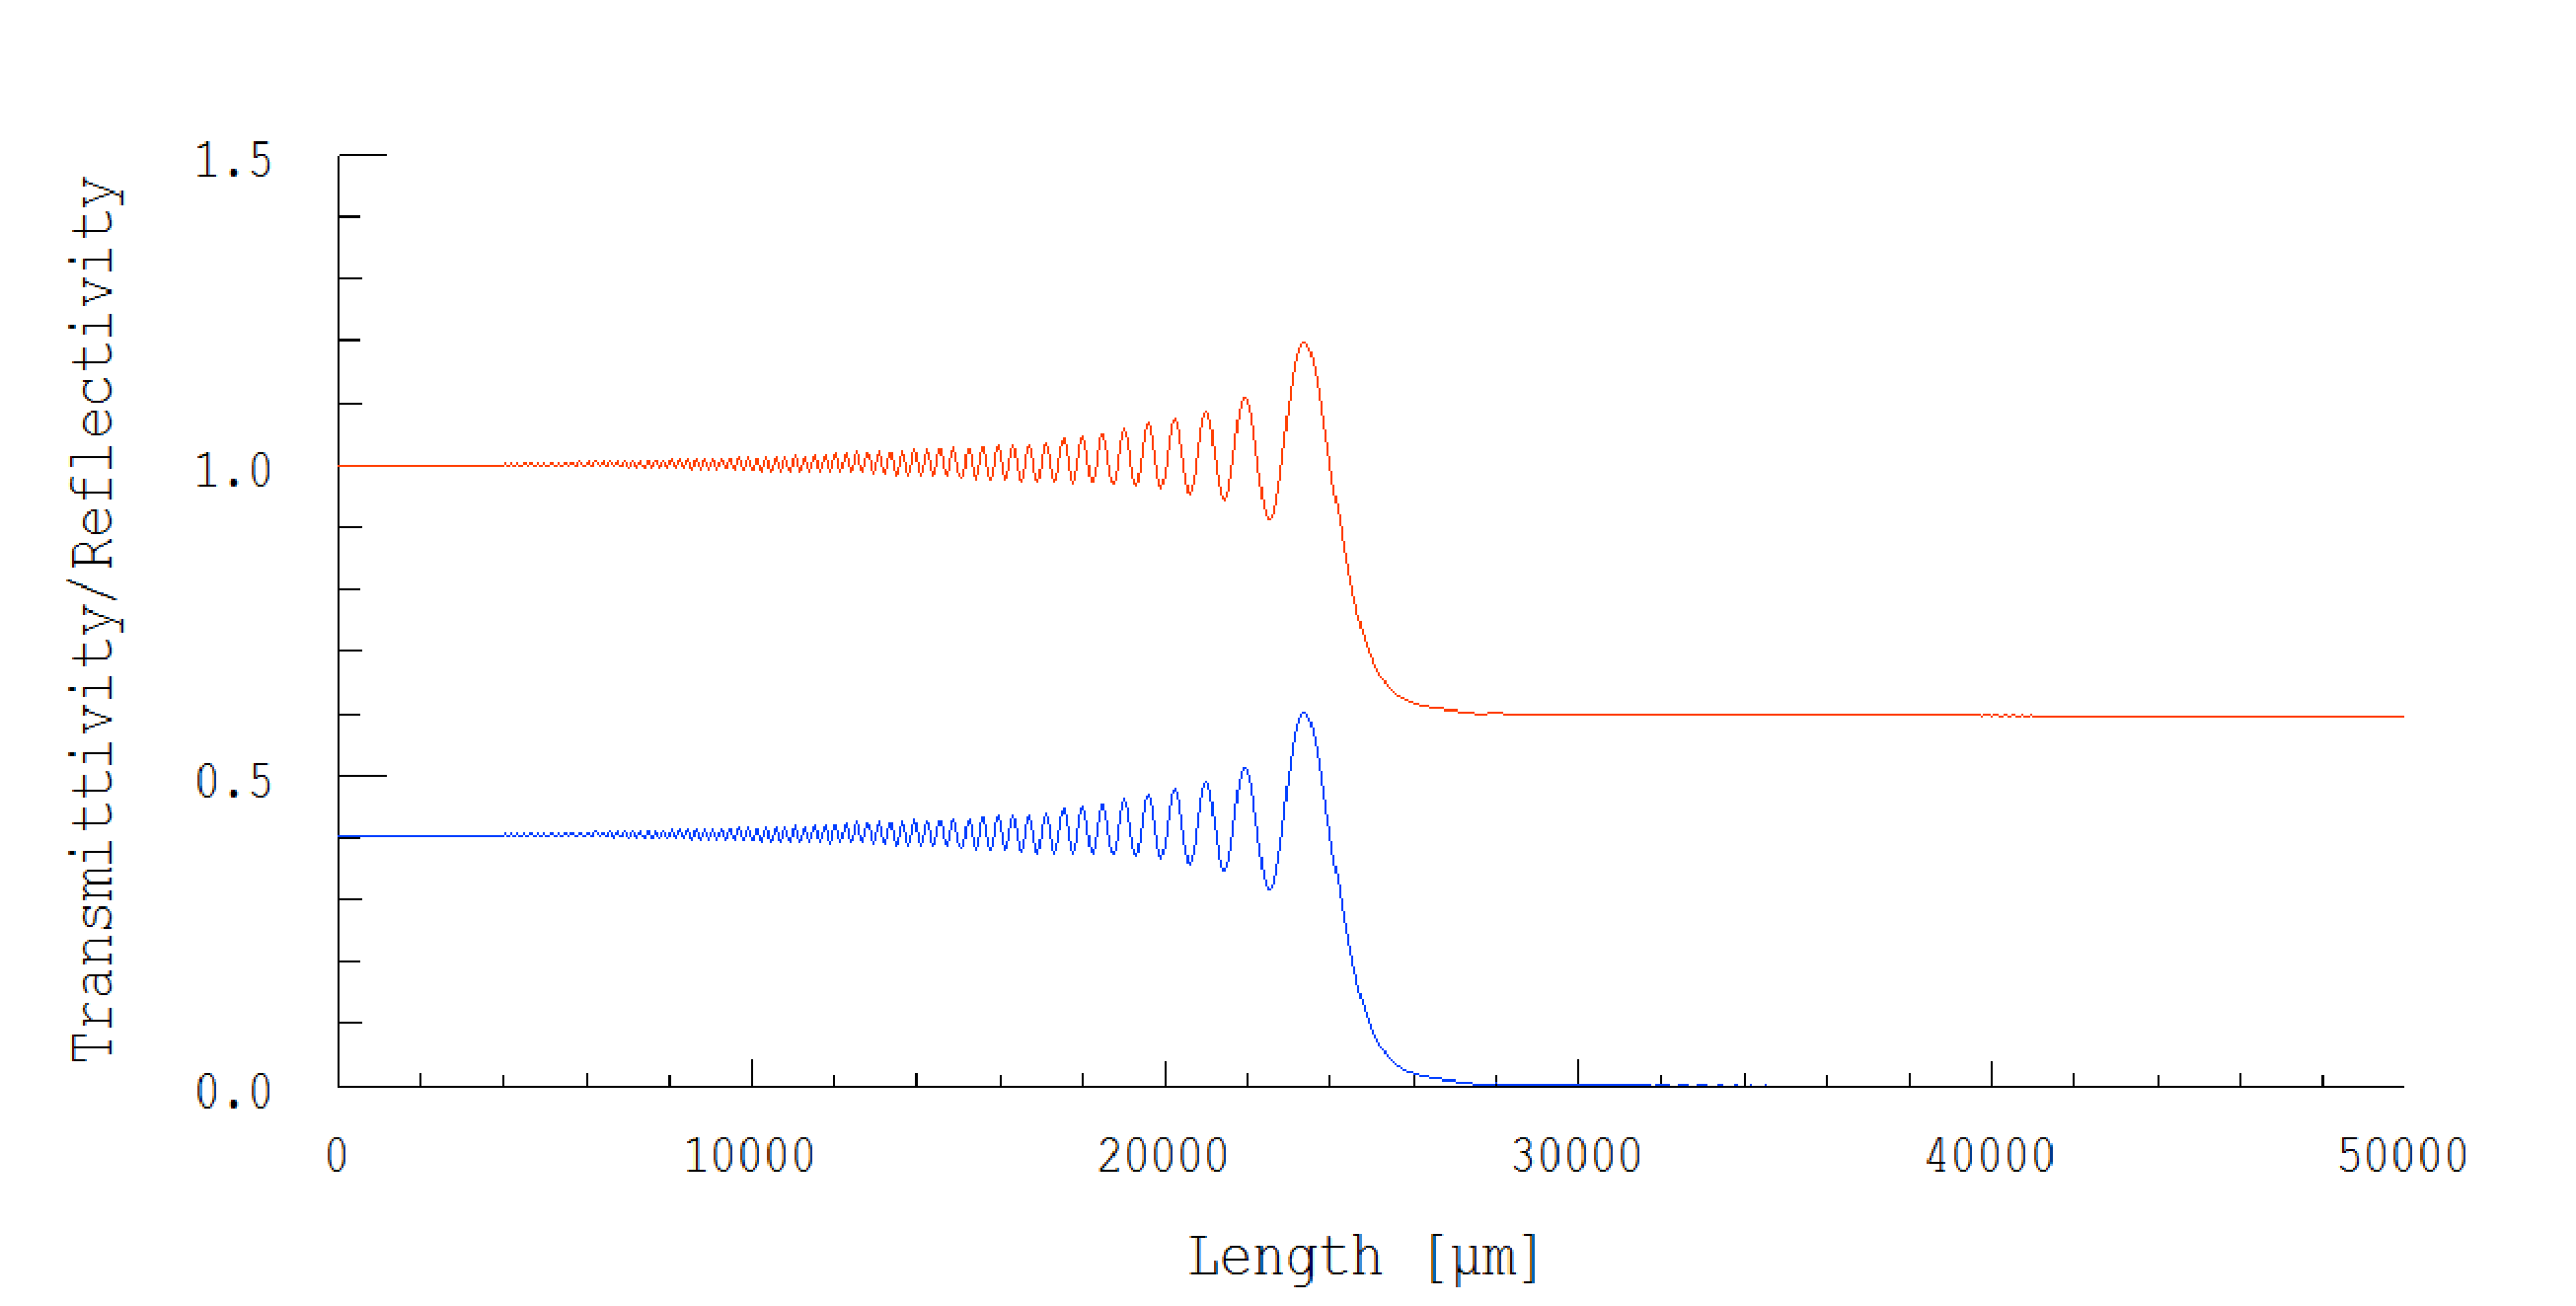
\includegraphics[scale=0.3]{fig_length_5.eps}\\
  \caption{График пропускания и отражения ВБР при длине решетки равной 5 мм. Верхний --- пропускание, нижний --- отражение.}\label{fig_length_5}
\end{figure}

\begin{figure}
  \centering
  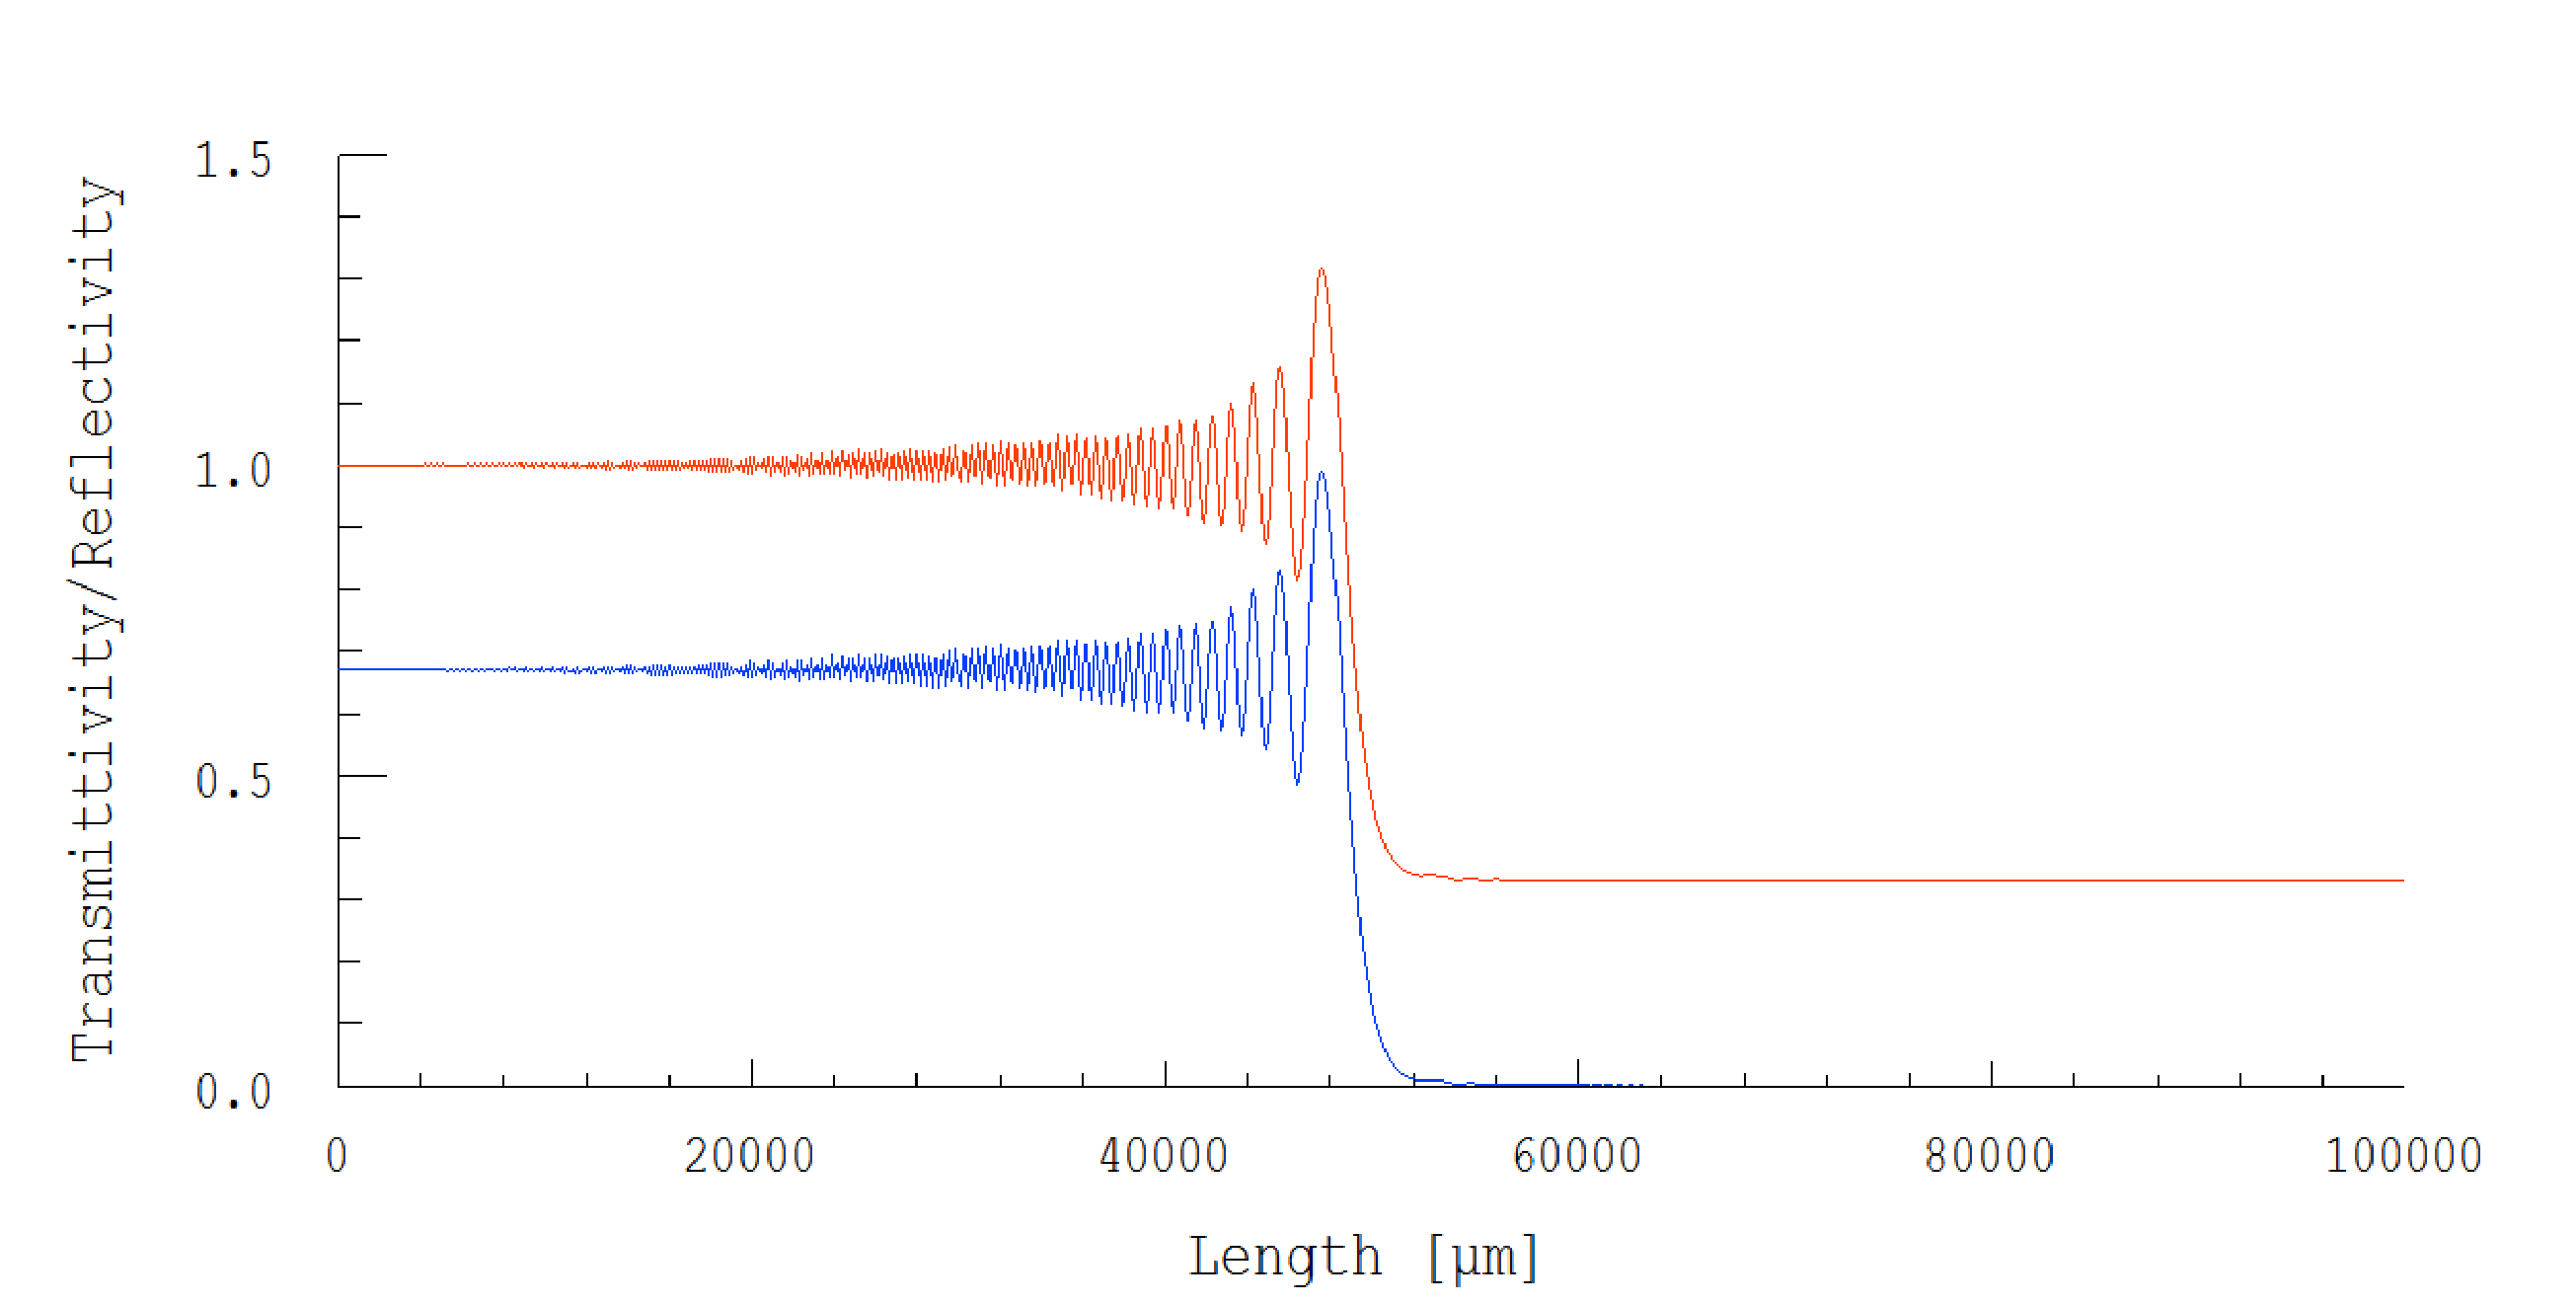
\includegraphics[scale=0.3]{fig_length_10.eps}\\
  \caption{График пропускания и отражения ВБР при длине решетки равной 10 мм. Верхний --- пропускание, нижний --- отражение.}\label{fig_length_10}
\end{figure}

\begin{figure}
  \centering
  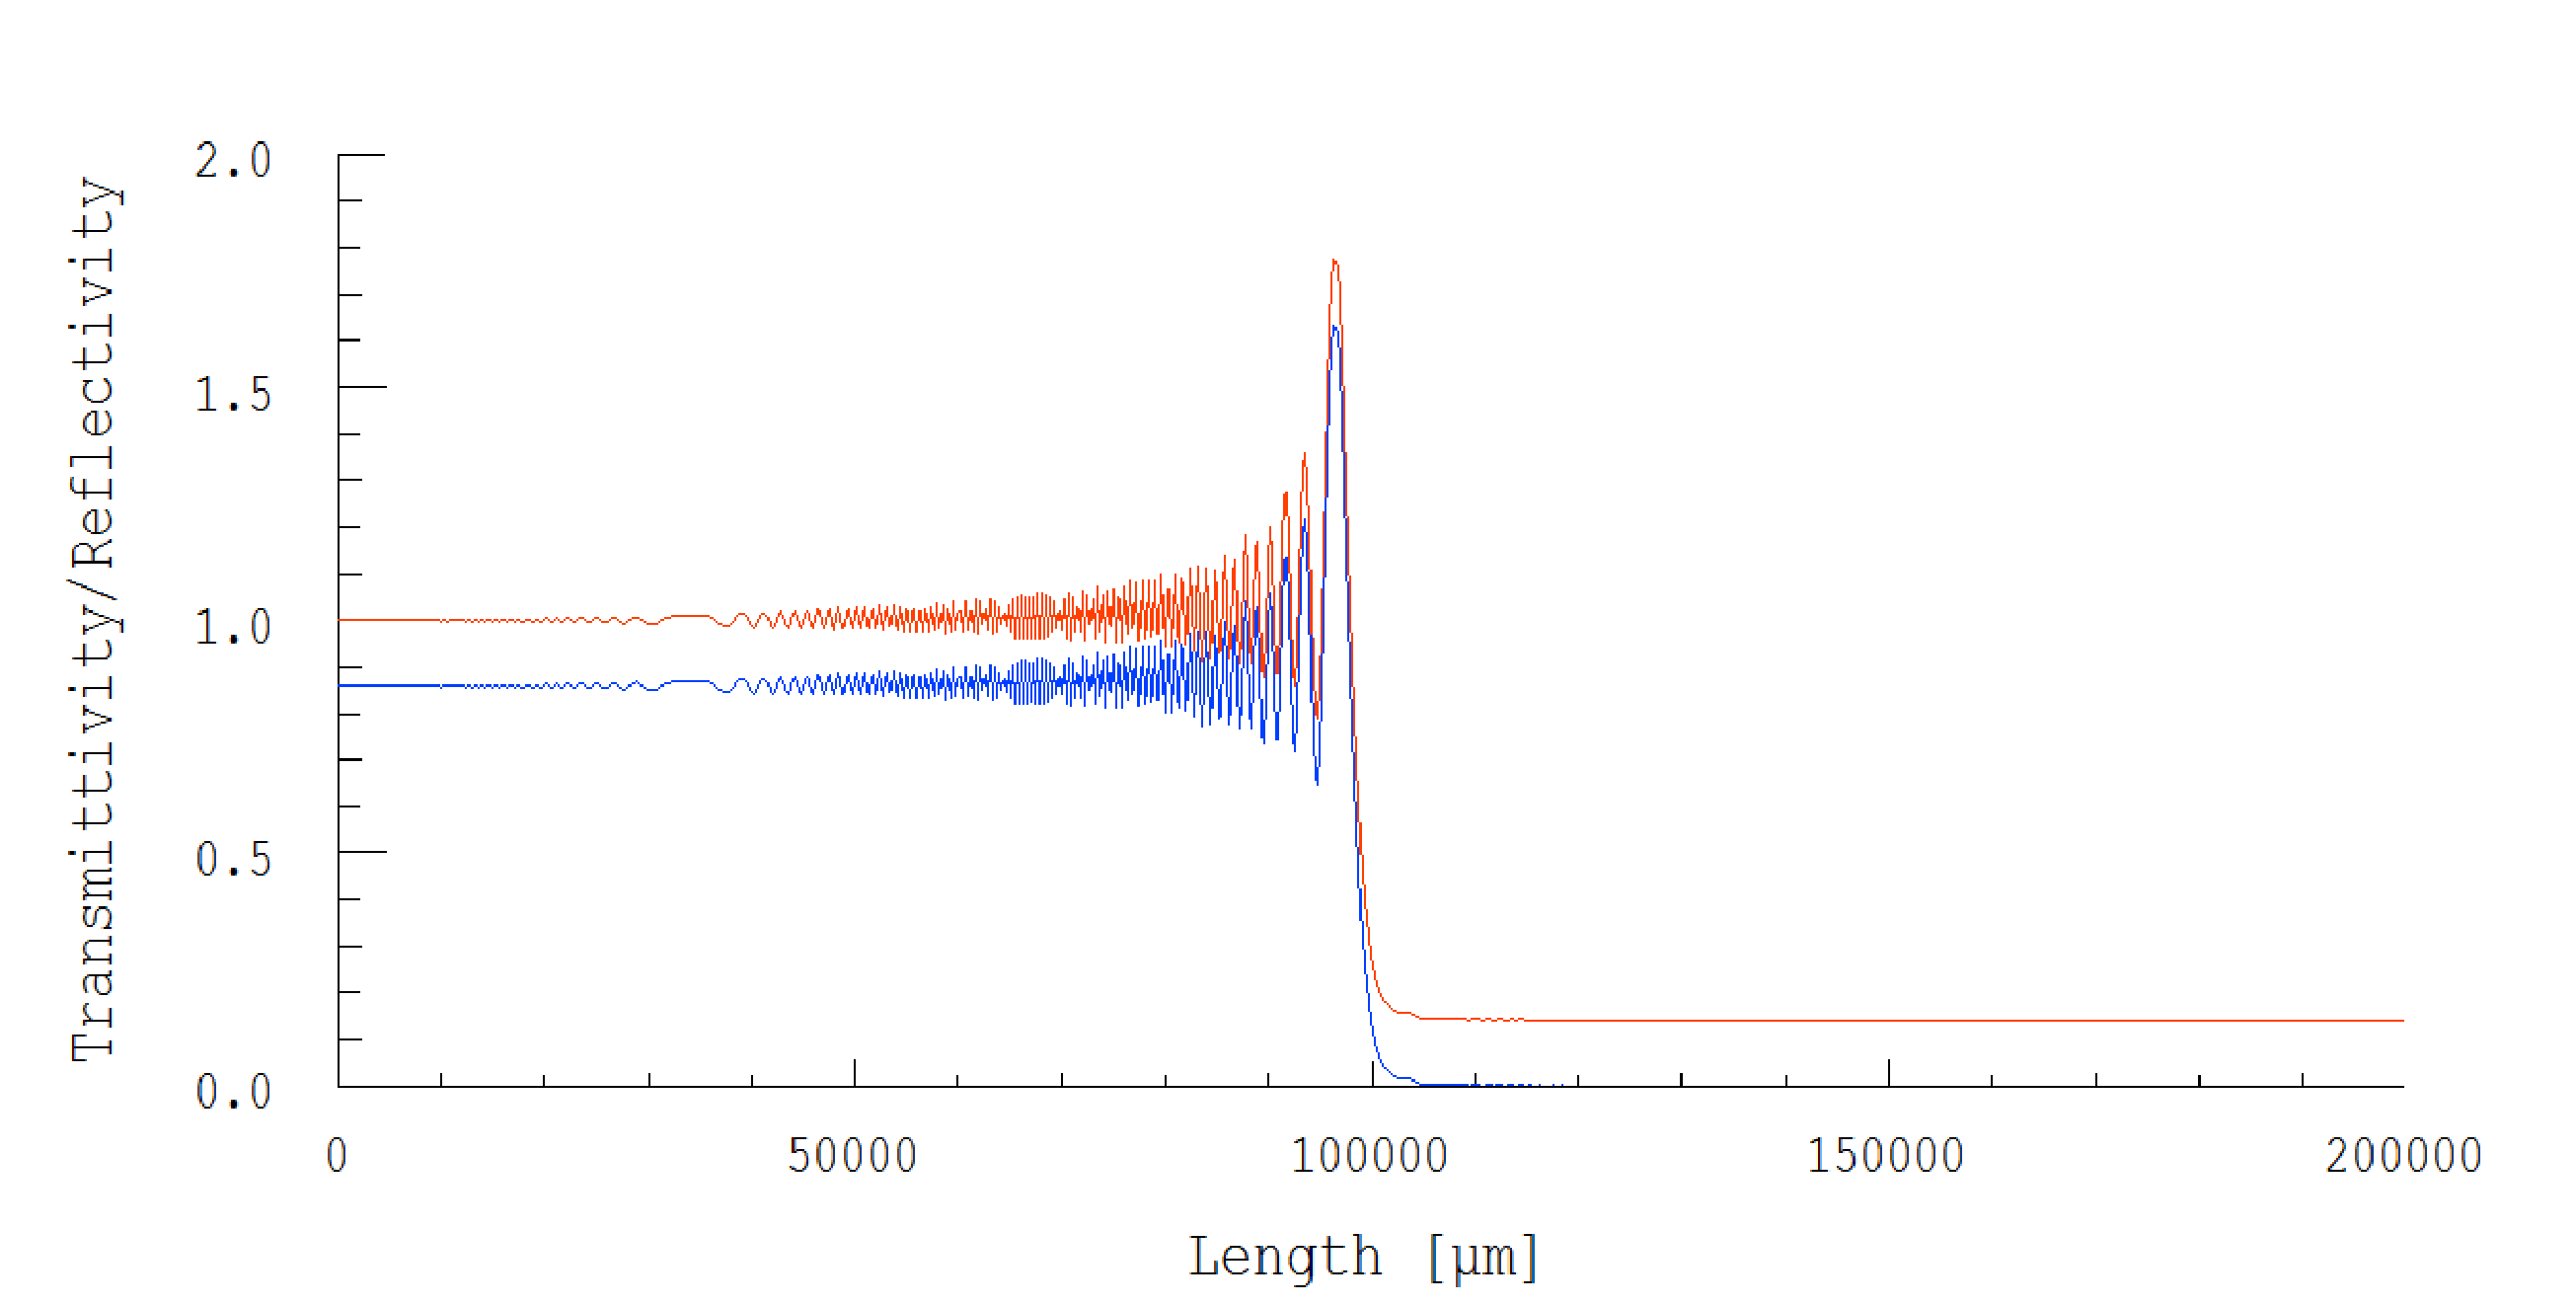
\includegraphics[scale=0.3]{fig_length_20.eps}\\
  \caption{График пропускания и отражения ВБР при длине решетки равной 20 мм. Верхний --- пропускание, нижний --- отражение.}\label{fig_length_20}
\end{figure}

\begin{figure}
  \centering
  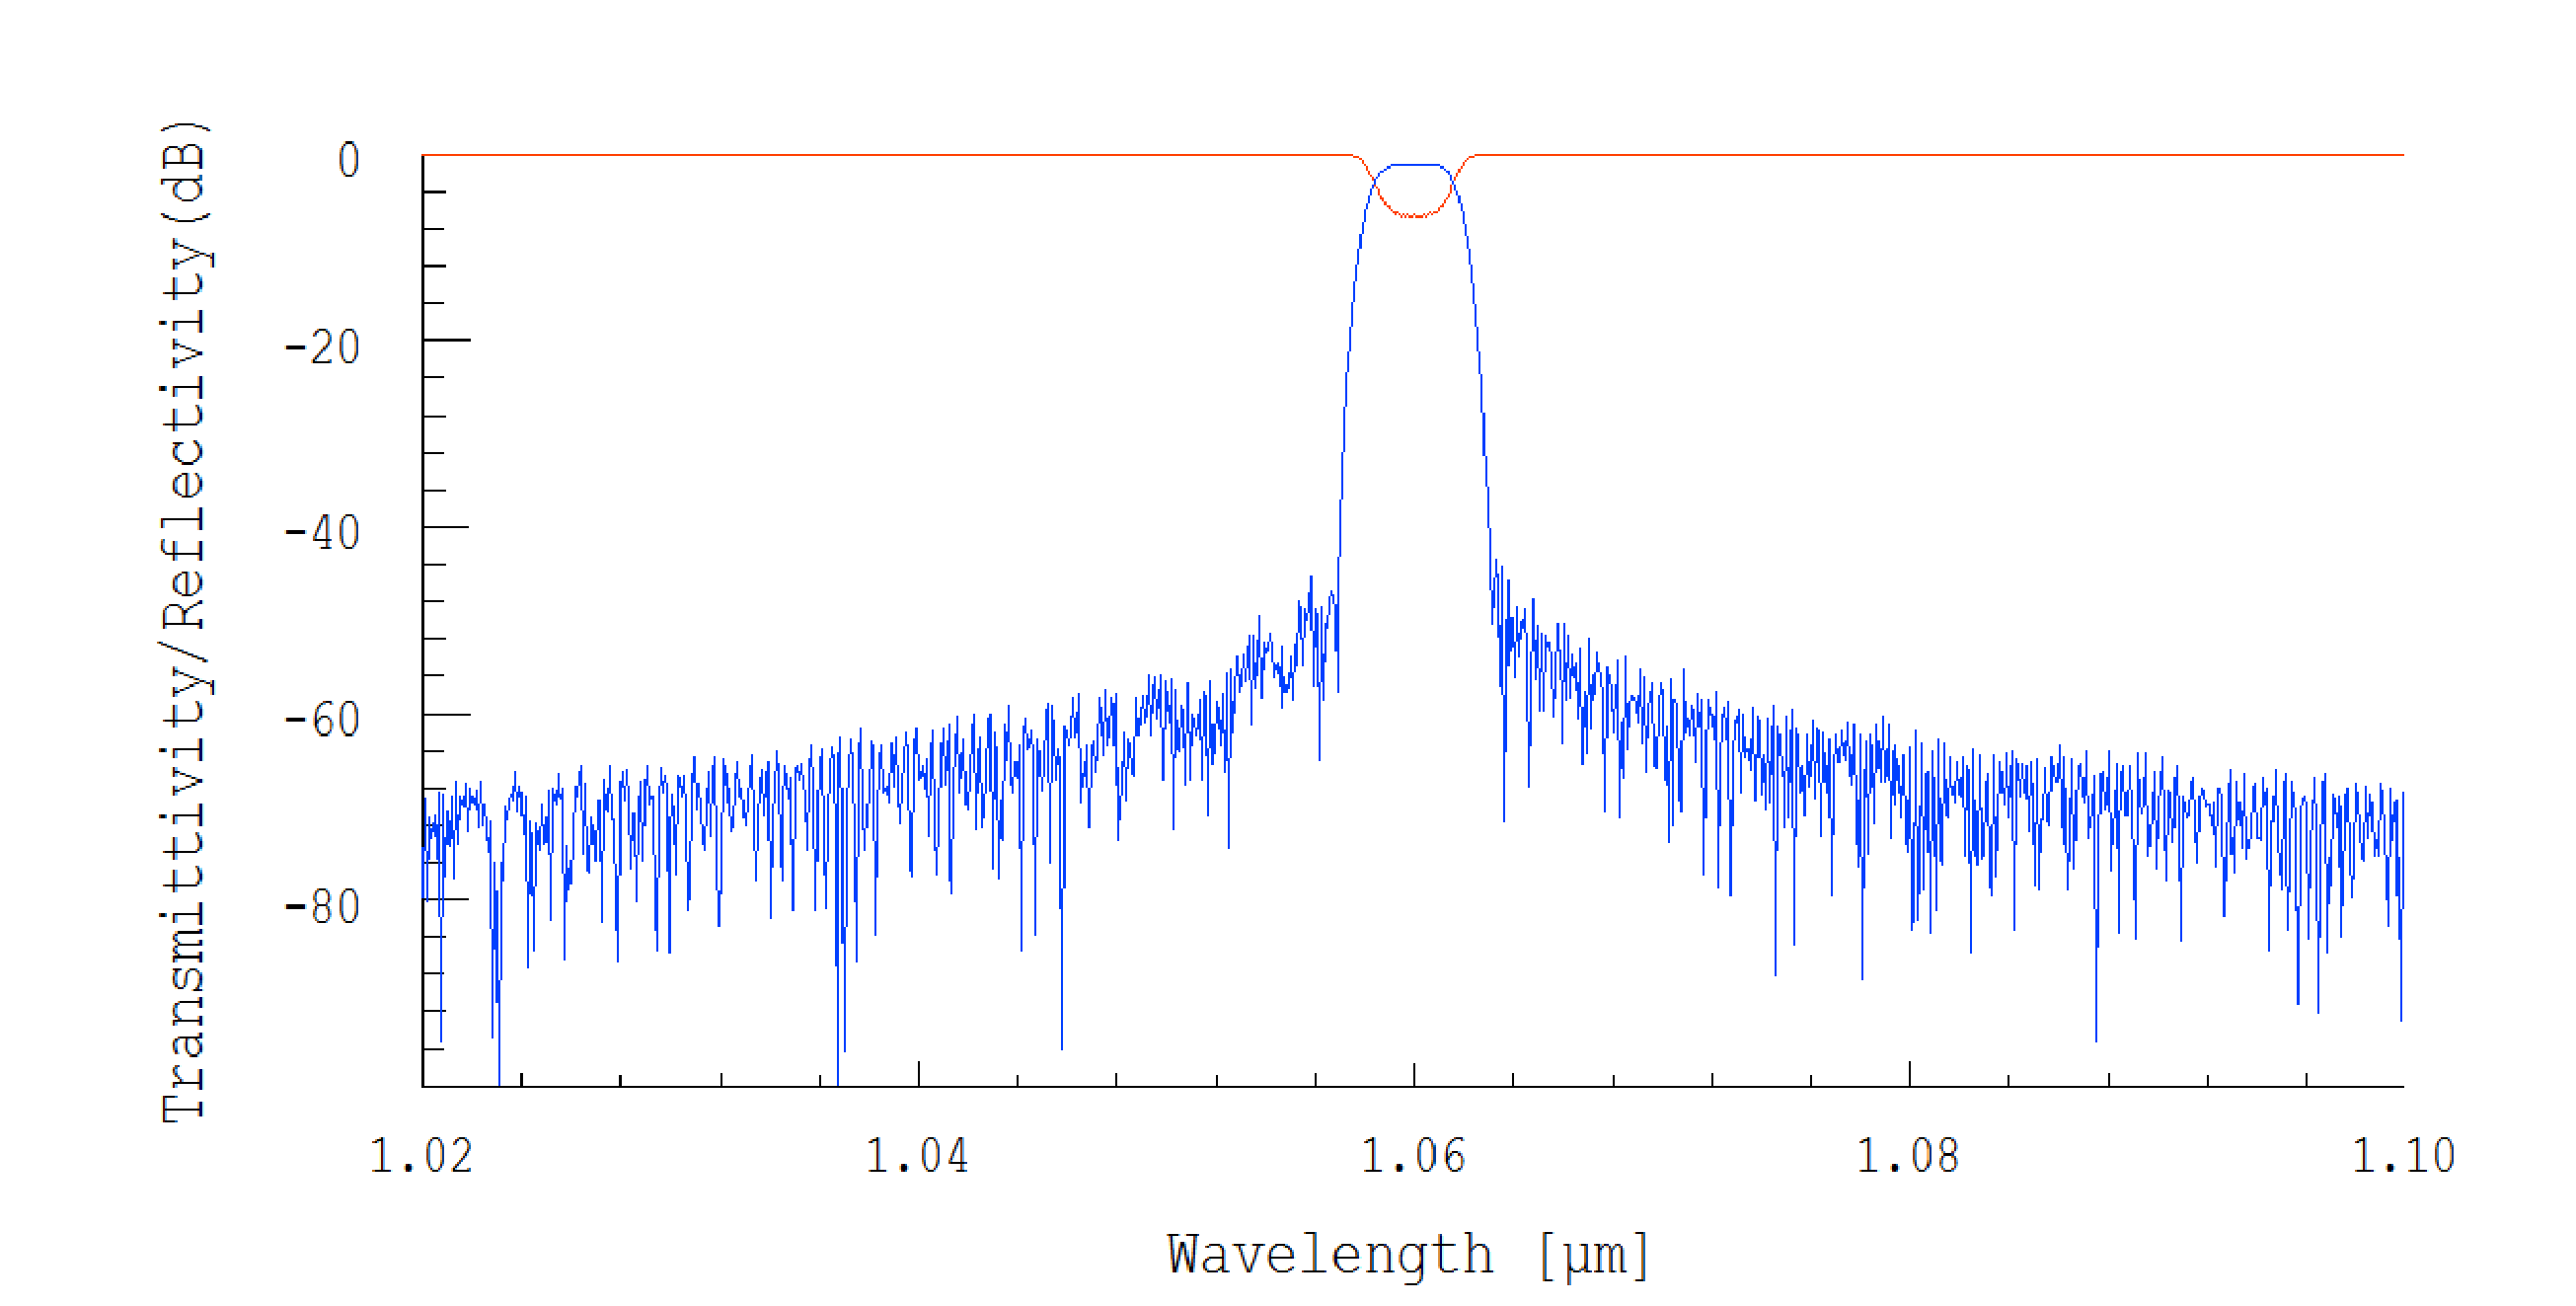
\includegraphics[scale=0.3]{fig_radial_linear.eps}\\
  \caption{Спектр пропускания и отражения ВБР при линейной зависимости коэффициента фоточувствительности от радиального $x$. Верхний --- пропускание, нижний --- отражение.}\label{fig_radial_linear}
\end{figure}

\begin{figure}
  \centering
  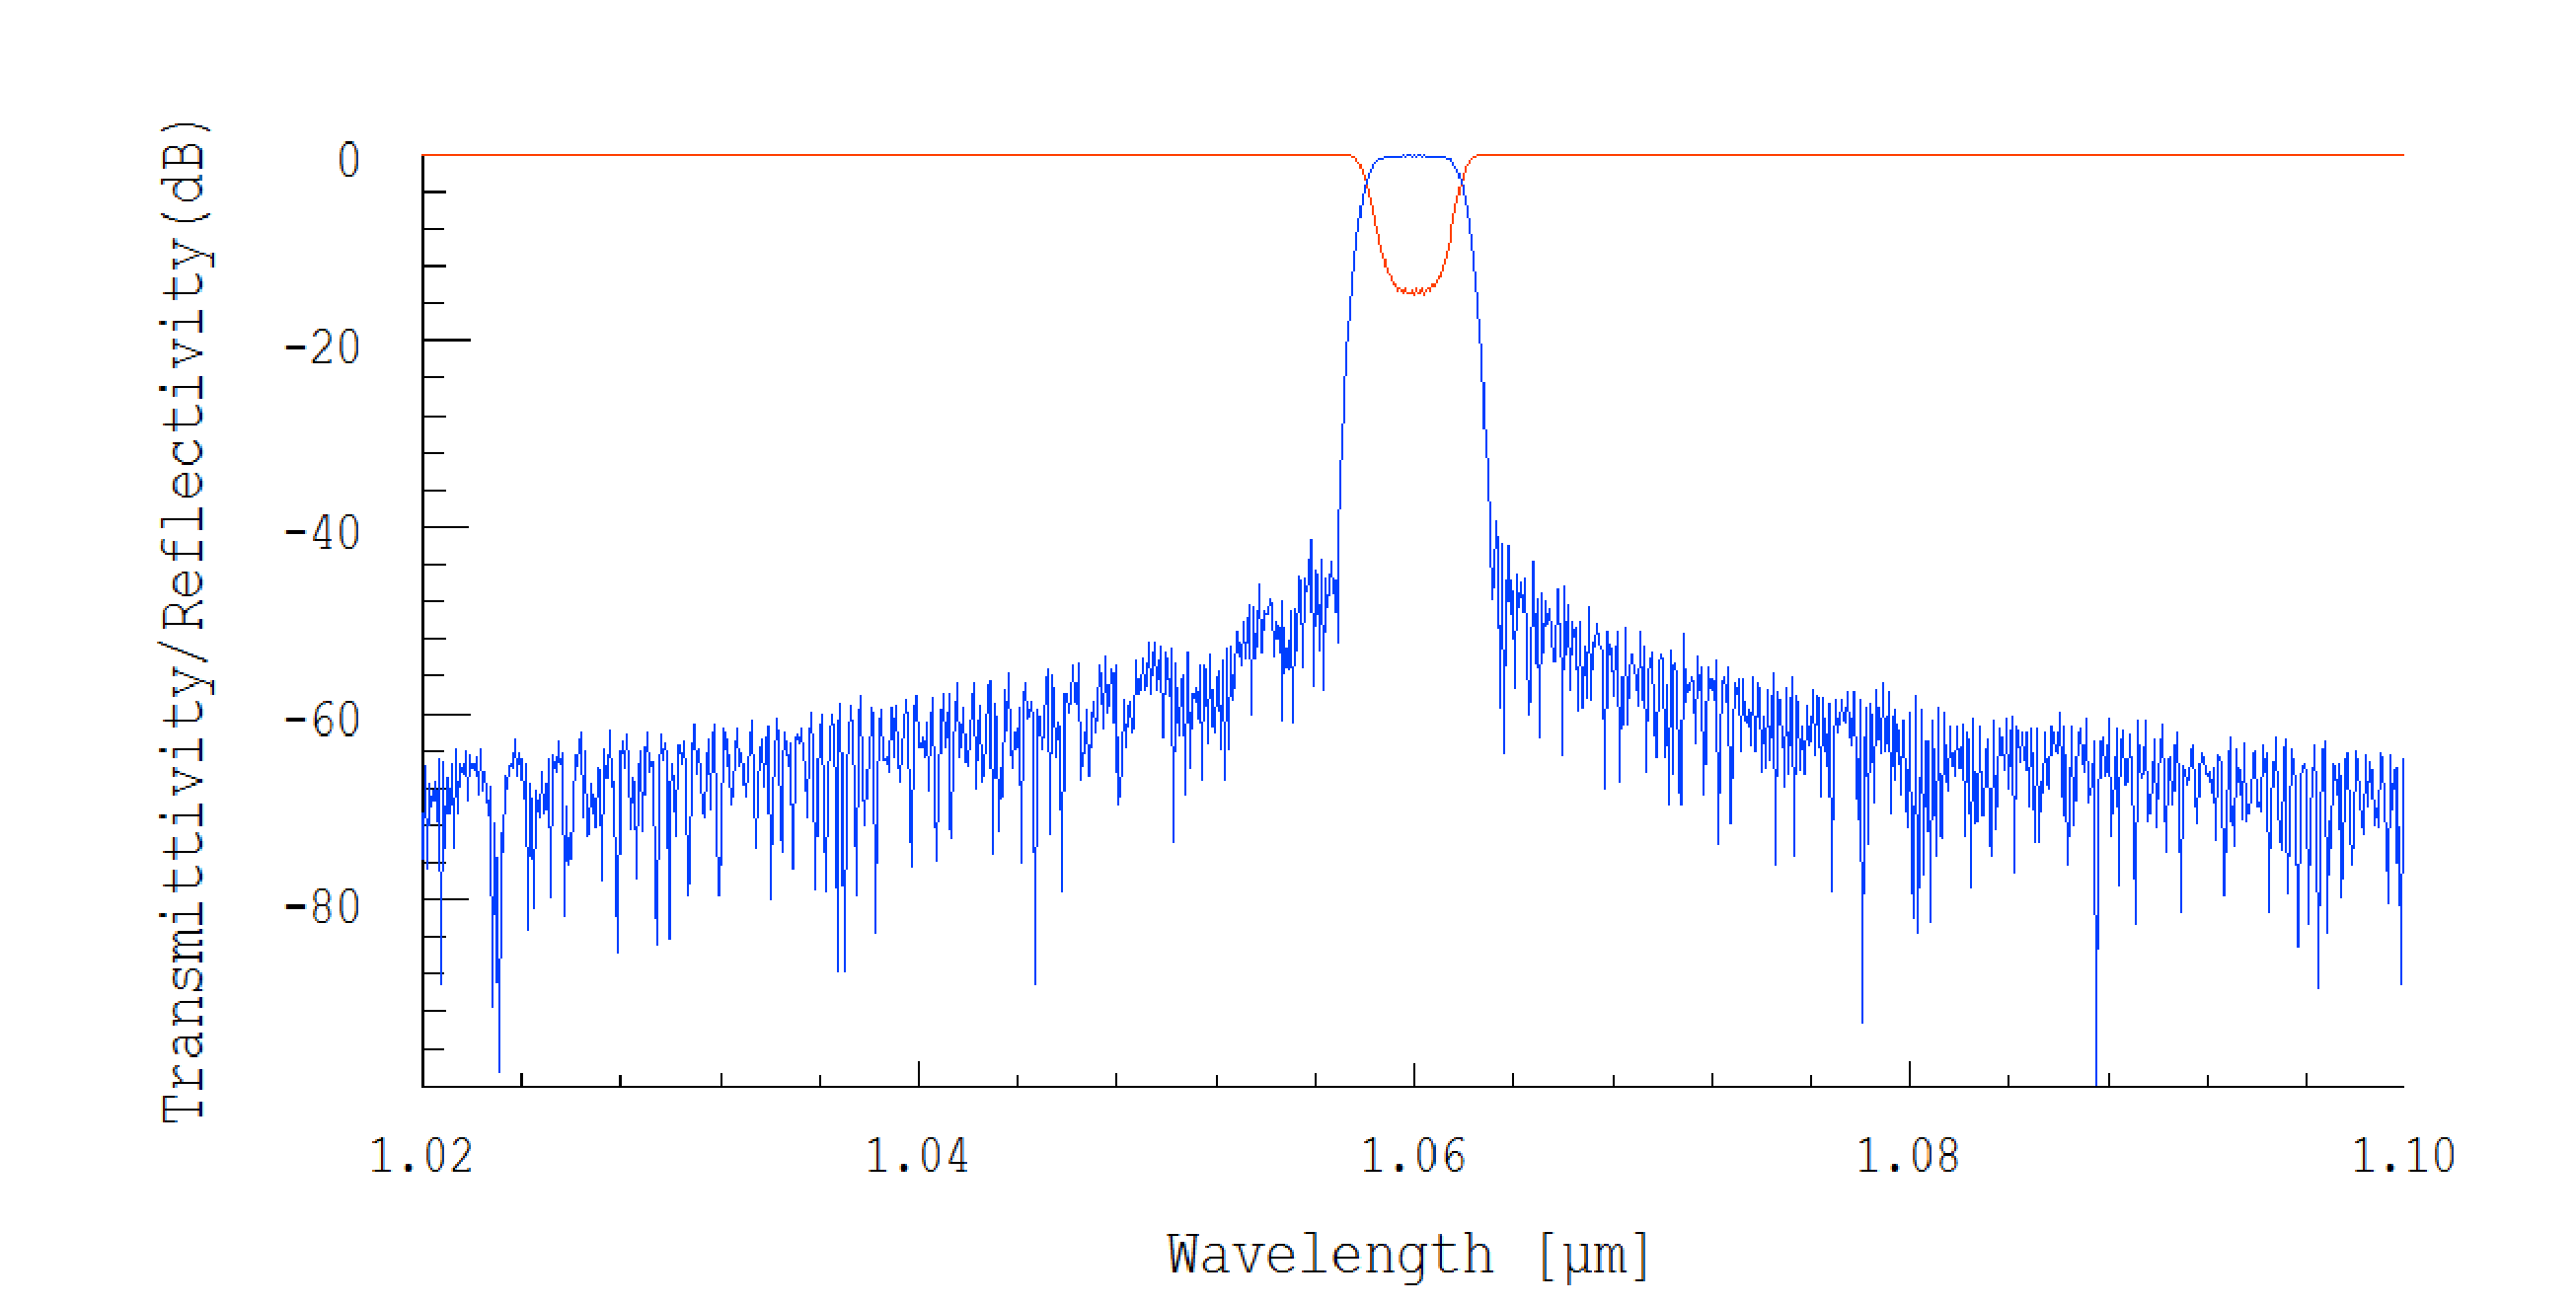
\includegraphics[scale=0.3]{fig_radial_parabolic.eps}\\
  \caption{Спектр пропускания и отражения ВБР при параболической зависимости коэффициента фоточувствительности от радиального $x$. Верхний --- пропускание, нижний --- отражение.}\label{fig_radial_parabolic}
\end{figure}

\begin{figure}
  \centering
  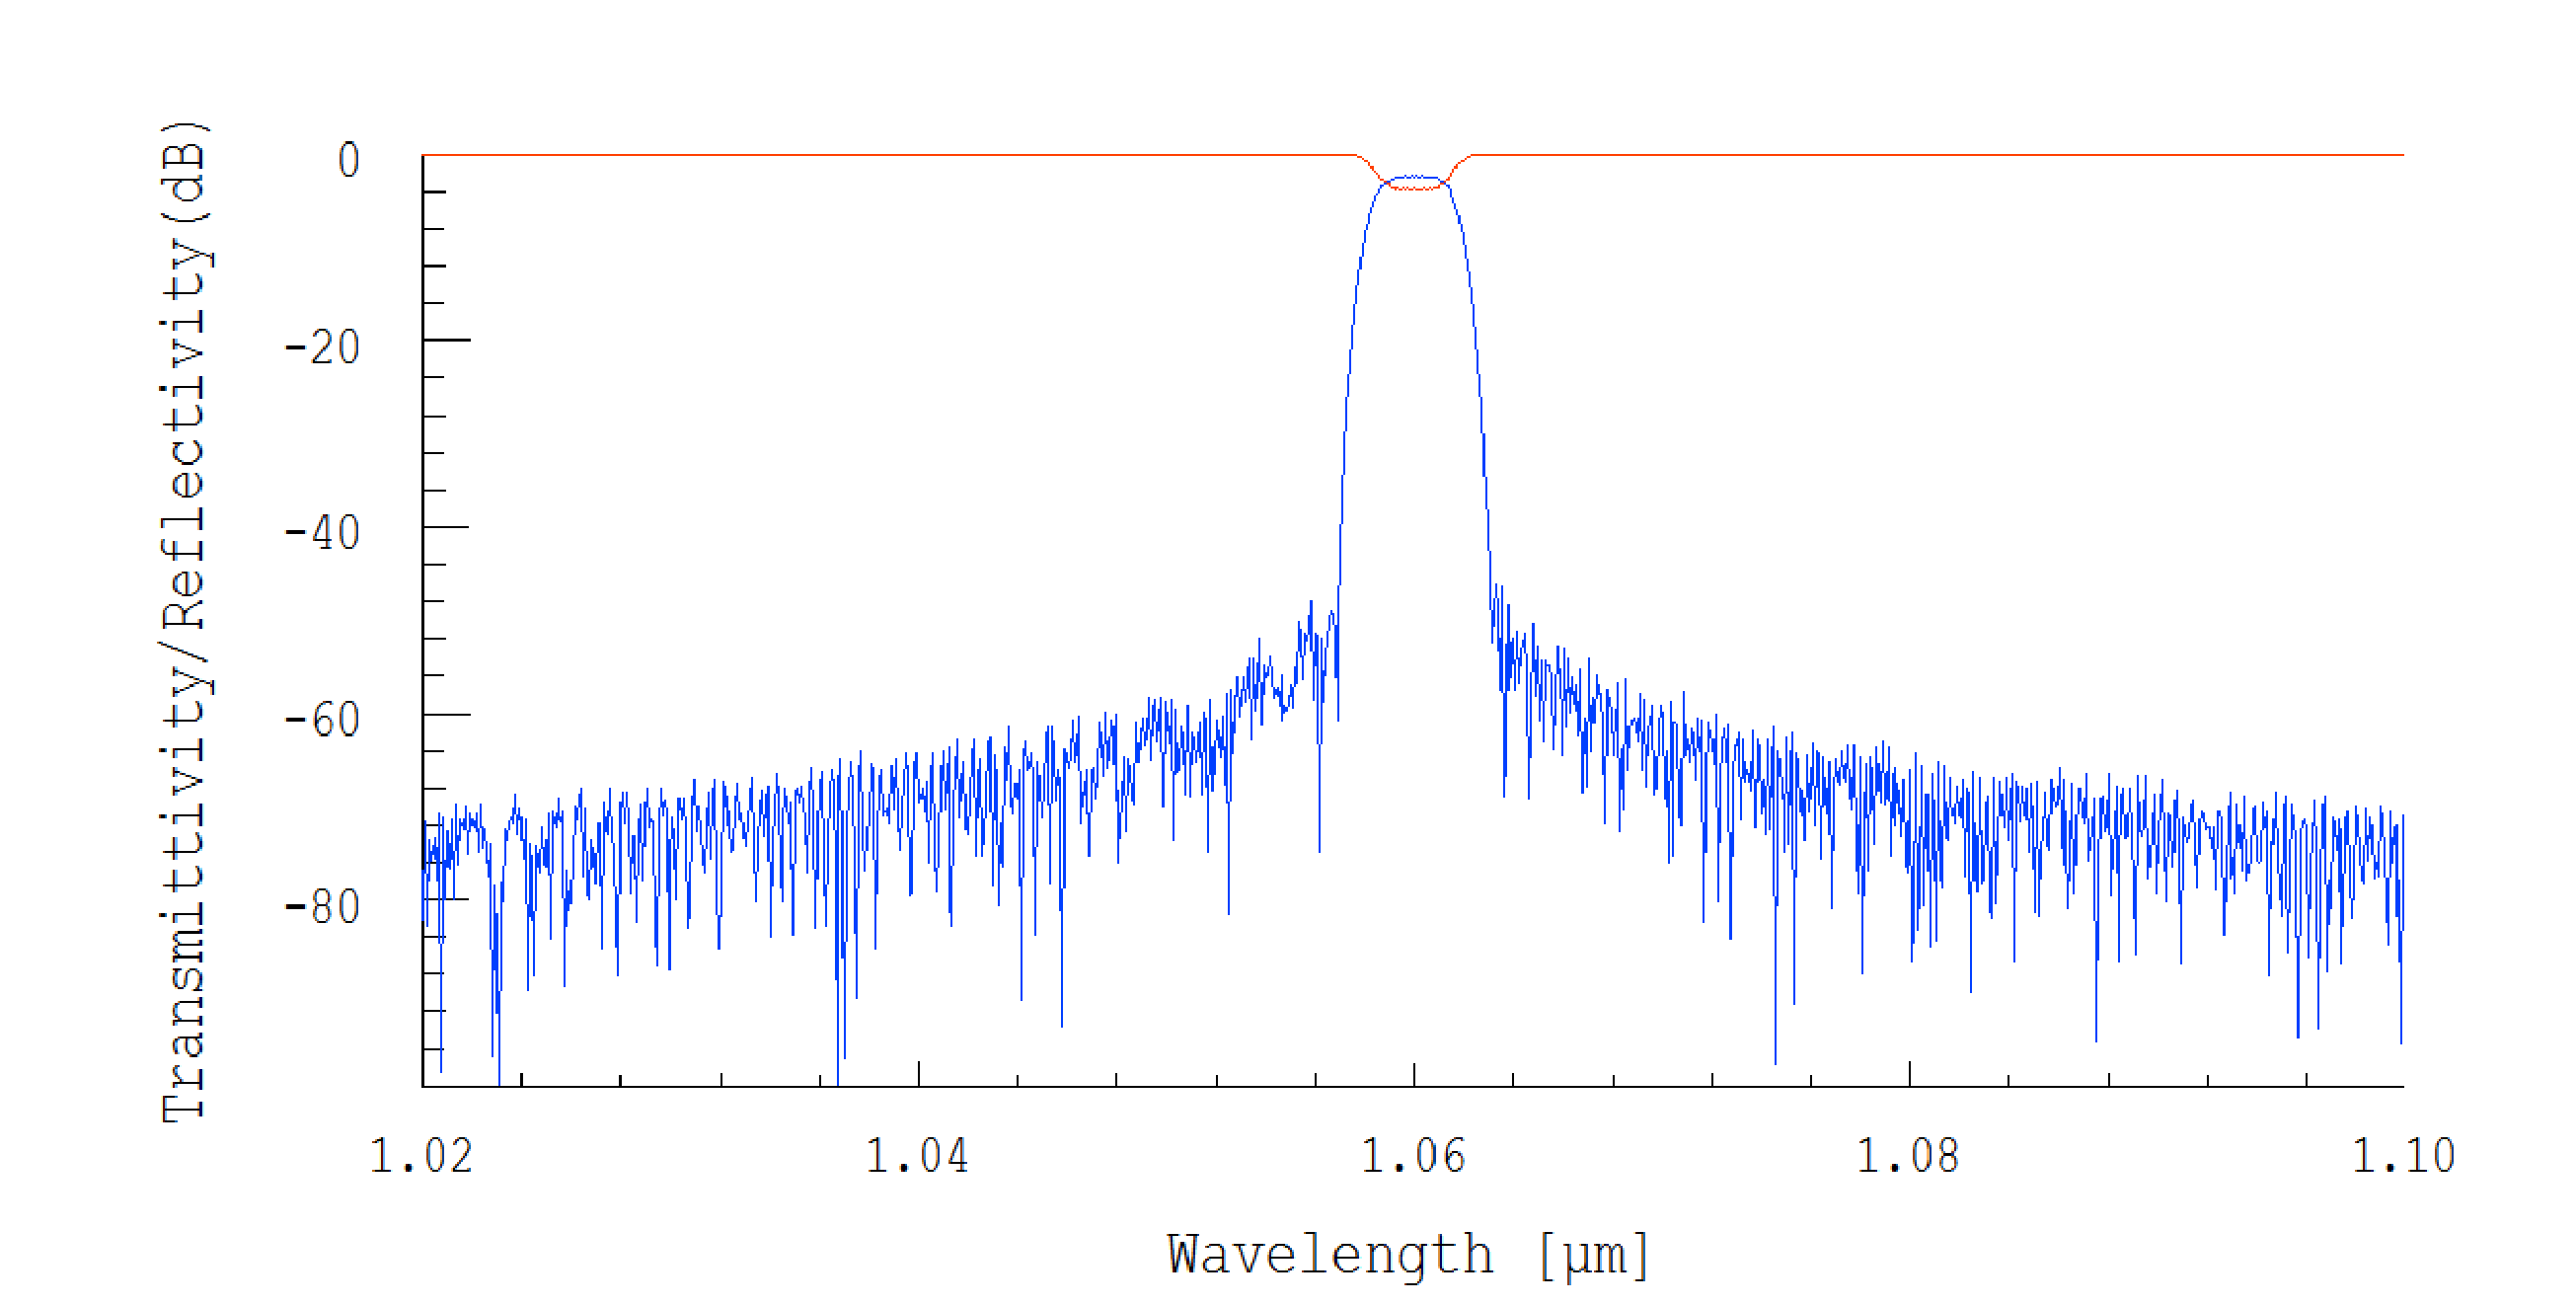
\includegraphics[scale=0.3]{fig_radial_exponent.eps}\\
  \caption{Спектр пропускания и отражения ВБР при экспоненциальной зависимости коэффициента фоточувствительности от радиального $x$. Верхний --- пропускание, нижний --- отражение.}\label{fig_radial_exponent}
\end{figure}

\begin{figure}
  \centering
  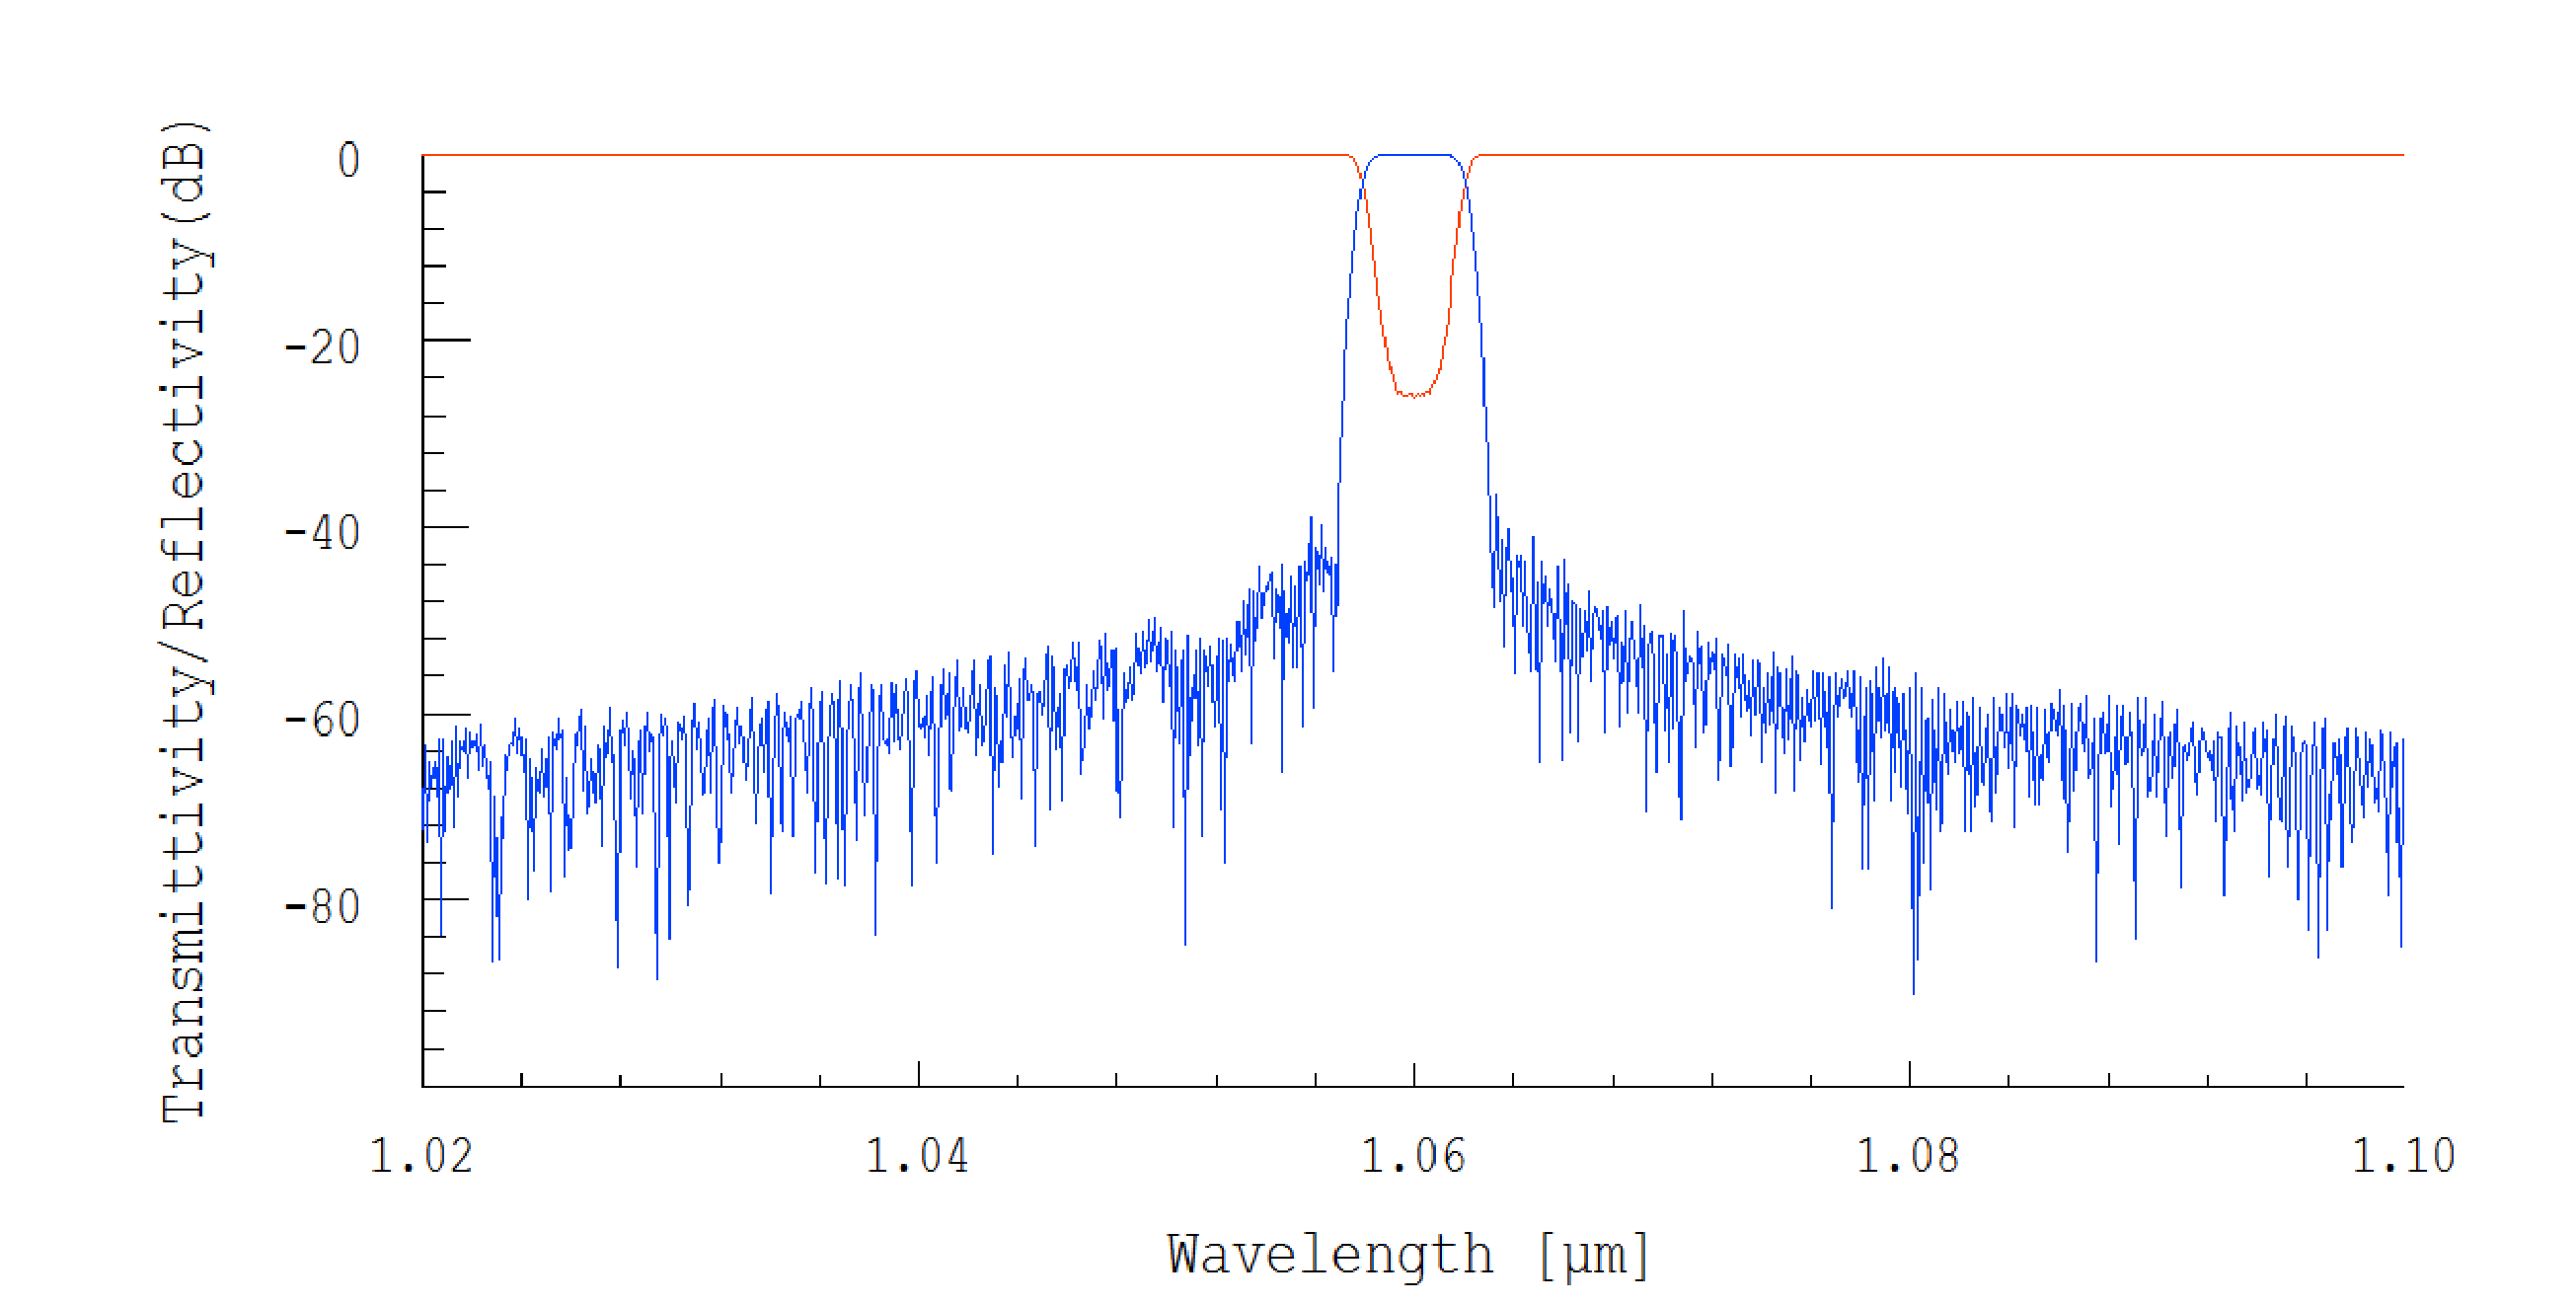
\includegraphics[scale=0.3]{fig_radial_gaussian.eps}\\
  \caption{Спектр пропускания и отражения ВБР при гауссовой зависимости коэффициента фоточувствительности от радиального $x$. Верхний --- пропускание, нижний --- отражение.}\label{fig_radial_gaussian}
\end{figure}

\begin{figure}
  \centering
  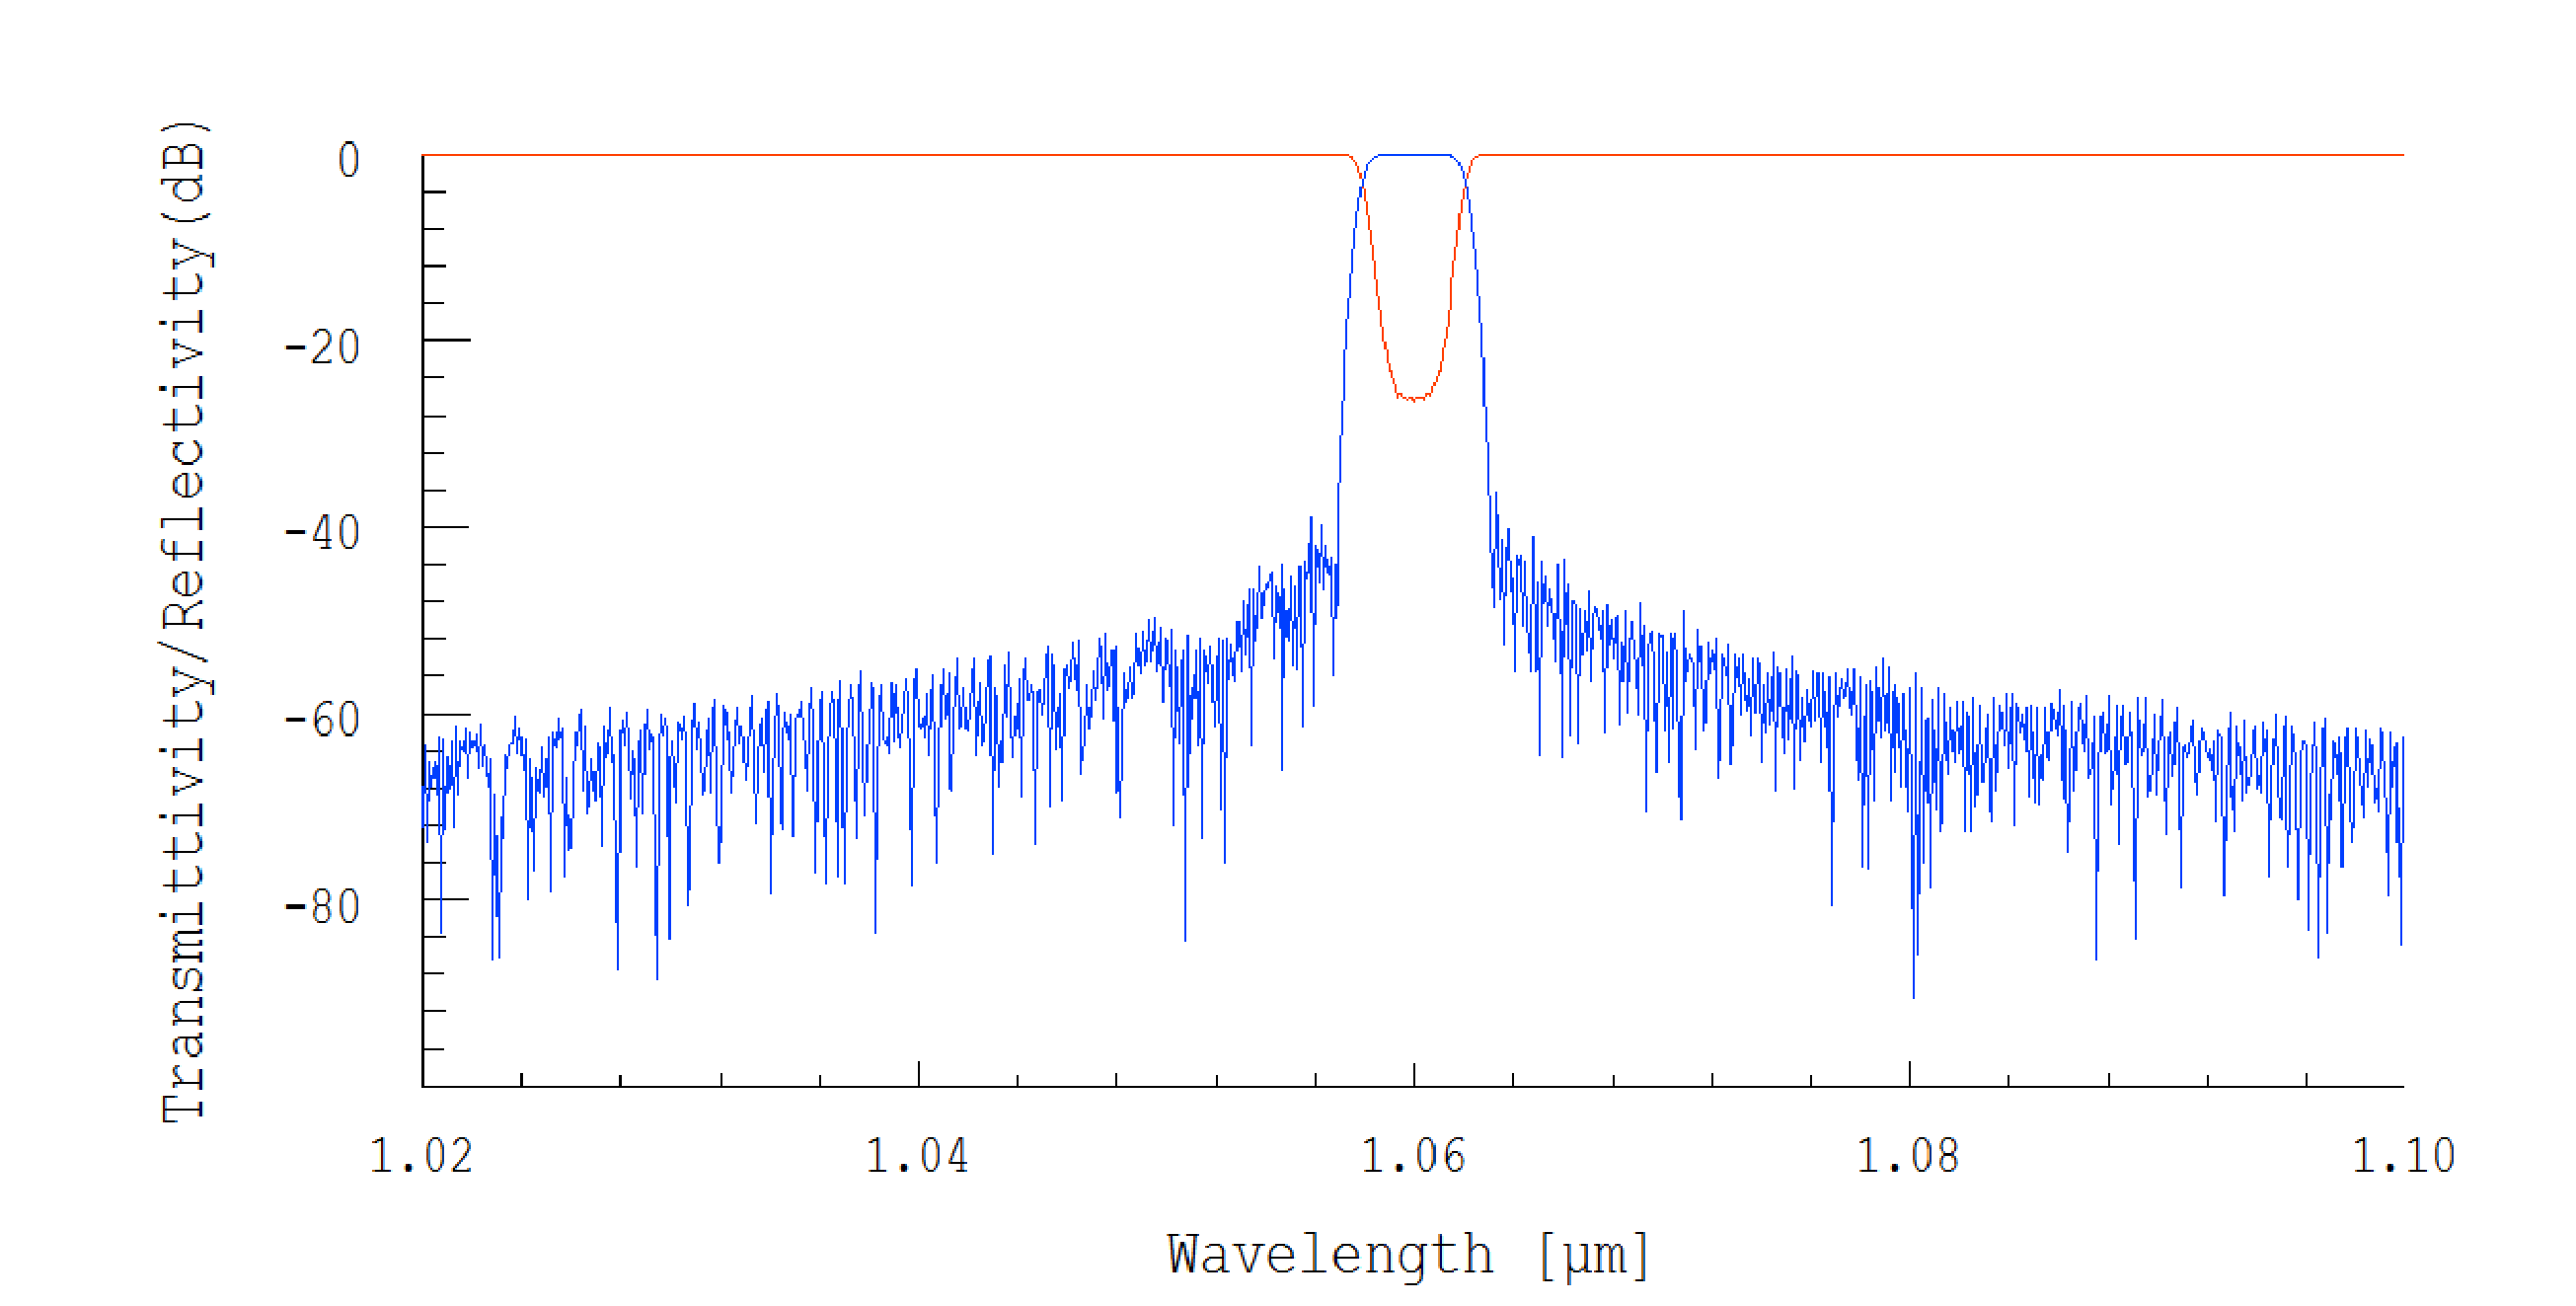
\includegraphics[scale=0.3]{fig_radial_alphapick.eps}\\
  \caption{Спектр пропускания и отражения ВБР при альфа-пик зависимости коэффициента фоточувствительности от радиального $x$. Верхний --- пропускание, нижний --- отражение.}\label{fig_radial_alphapick}
\end{figure}

\begin{figure}
  \centering
  \includegraphics[scale=0.3]{fig_radial_alphadip.eps}\\
  \caption{Спектр пропускания и отражения ВБР при альфа-провал зависимости коэффициента фоточувствительности от радиального $x$. Верхний --- пропускание, нижний --- отражение.}\label{fig_radial_alphadip}
\end{figure}

Мы не будем здесь приводить графики отражения и пропускания ВБР в расчете на единицу мощности проходящего излучения, а сведем все значения отражений решеток в таблицу.

\begin{tabular}{|c|c|}
\hline \rule[-2ex]{0pt}{5.5ex} \textbf{Профиль фоточувствительности} & \textbf{Коэффициент отражения} \\ \hline
\hline \rule[-2ex]{0pt}{5.5ex} Линейный & 77\% \\
\hline \rule[-2ex]{0pt}{5.5ex} Параболический & 97\% \\
\hline \rule[-2ex]{0pt}{5.5ex} Экспоненциальный & 56\% \\
\hline \rule[-2ex]{0pt}{5.5ex} Гауссовый & 99\% \\
\hline \rule[-2ex]{0pt}{5.5ex} $\alpha$-пик & 99\% \\
\hline \rule[-2ex]{0pt}{5.5ex} $\alpha$-провал & 99\% \\
\hline
\end{tabular}

\bigskip
Исходя из полученных данных о коэффициенте отражения ВБР при различных видах профиля фоточувствительности волокна, можно предположить, что отражение зависит не от вида функции, а от ее интегральной суммы (площади под графиком функции). Из этого вполне логично вытекает результат абсолютно одинаковых по выходным характеристикам ВБР при профиле фоточувствительности альфа-пик и альфа-провал. У экспоненциальной функции интегральная сумма минимальна, поэтому и решетка имеет наименьший коэффициент отражения.

%\newpage
%=======================================================================================
%=======================================================================================

\section{Экспериментальная отработка технологического процесса изготовления фотоиндуцированных решеток показателя преломления методом фазовой маски}
\label{sec:fbg_exper}

В последние годы в волоконной оптике активно развивается направление, связанное с получением распределенных структур показателя преломления (ПП) в сердцевине световода. Как правило, такие структуры создаются в германосиликатных световодах путем их бокового облучения достаточно мощным УФ излучением, длина волны которого попадает в полосу поглощения германиевых кислородно-дефицитных центров с максимумом при $\lambda = 242$ нм~\cite{fbg_1}. Получаемые при этом внутриволоконные решетки ПП обладают такими спектральными характеристиками, которые позволяют эффективно использовать их во многих практических применениях (зеркала волоконных лазеров, датчики, фильтры и др.)~\cite{fbg_2}.

Важной стратегической задачей при разработке мощных волоконных лазеров является наличие собственной локализованной технологии создания волоконных элементов лазера и технологии создания волоконных брэгговских решеток в частности. Гибкость в отношении требуемых и получаемых характеристик, а также удешевление стоимости волоконного лазера за счет собственного производства волоконных компонентов позволит конкурировать с ведущими мировыми производителями как по себестоимости, так и по качеству.

Ранее в лаборатории 57-5 был опубликован отчет~\cite{fbg_3} с обзором методов записи ВБР, их типами, а также с кратким описанием явления фоточувствительности. Также в отчете дано обоснование выбора метода фазовой маски для реализации технологии записи ВБР. Кроме того, в отчете~\cite{fbg_4} выполнен расчет спектра отражения волоконных брэгговских решеток, что крайне важно при подборе оптимальных параметров ВБР для получения желаемых спектральных характеристик.

Таким образом, целями представленной работы являются:
\begin{enumerate}
    \item Отработка технологического процесса изготовления волоконных брэгговских решеток (ВБР) методом фазовой маски.
    \item Изготовление опытного образца глухой (HR) и выходной (HT) ВБР.
\end{enumerate}

\subsection{Установка формирования и индуцирования периодической структуры ВБР}
\label{sub:fbg_exper_compex}

На базе установки VarioLas, в основе которой лежит эксимерный лазер CompexPro 110 от компании Coherent (США), собрана установка для записи волоконных брэгговских решеток. Параметры эксимерного лазера приведены в таблице~\ref{tbl:nrl_1}.

\begin{table}
  \centering
  \parbox{15cm}{\caption{Параметры эксимерного лазера CompexPro 110.}\label{tbl:nrl_1}}
  \begin{tabular}{| p{6cm} | p{9cm} |}
  \hline
        Параметр  & Значение \\
  \hline
  \hline
        Длина волны излучения &  248 нм \\
        Эксимерная смесь &  KrF (0,12 \% F2, 2,3 \% He, 3,03 \% Kr, 94,55 \% Ne) \\
        Частота следования импульсов &  до 100 кГц \\
        Длительность импульсов &  20 нс \\
        Макс. энергия импульса &  400 мДж (при 5 Гц и 30 кВ) \\
        Макс. средняя мощность &  30 Вт (при 100 Гц и 26 кВ) \\
        Размер выходного пучка (верт.) &  24 мм \\
        Размер выходного пучка (гор.) &  10 мм \\
        Расходимость пучка (верт.) &  3 мрад \\
        Расходимость пучка (гор.) &  1 мрад \\
        Стабильность энергии генерации &  1 \% \\
  \hline
  \end{tabular}
\end{table}

Оптика в оптическом тракте была перемонтирована и установлена таким образом, чтобы получить требуемое техпроцессом пятно облучения (шириной 30 мм и минимальной высотой) на фоточувствительном волокне. Схема расположения оптических элементов показана на рис.~\ref{img:fbg_tech_1}.

\begin{figure}[ht]
  \centering
  \includegraphics[width=0.5\linewidth]{fbg_tech_1.png}
  \caption{Оптический тракт комплекса записи волоконных брэгговских решеток.}
  \label{img:fbg_tech_1}
\end{figure}

Общий вид установки с лазером показана на рис.~\ref{img:fbg_tech_2}.
\begin{figure}[ht]
  \centering
  \includegraphics[scale=1.2]{fbg_tech_2.png}
  \caption{Общий вид установки для записи волоконных брэгговских решеток (без защитного бокса в зоне записи решеток).}
  \label{img:fbg_tech_2}
\end{figure}

Для точного позиционирования волокна и маски в зоне облучения лазером из имеющихся автоматических подвижек фирмы Thorlabs была собрана двухкоординатная подвижка с держателями волокна и маски. Вертикальная координата была настроена на оптимальное значение и жестко зафиксирована. В процессе дальнейшей работы выяснилось, что собранная схема не обеспечивает требуемую точность позиционирования и обладает низкой повторяемостью результатов. Поэтому была предложена новая монолитная схема монтажа маски и волокна (см. рис.~\ref{img:fbg_tech_3}).
\begin{figure}
  \centering
  \includegraphics[scale=0.6]{fbg_tech_3}
  \caption{Подложка для монтажа маски и волокна.}
  \label{img:fbg_tech_3}
\end{figure}

Однако, в предложенной схеме монтаж маски происходит непосредственно на фоточувствительное волокно, очищенное от оболочки. Отсутствие жесткой фиксации волокна и маски относительно друг друга в ходе записи приводило к затиранию решетки вероятно из-за наличия микровибраций и микроперемещений между волокном и маской. Фиксация волокна на держателе и самой маски с помощью специальных магнитных зажимов решило эту проблему, но при демонтаже волокна после записи извлечь волокно стало крайне сложно в силу хрупкости очищенного волокна. Кроме этого, появилась необходимость в процессе записи подогревать волокно и охлаждать (термостабилизировать) фазовую маску. В связи с этим конструкция держателя волокна и маски находится на стадии инженерной проработки.

\subsection{Описание технологического процесса записи ВБР}
\label{sub:fbg_exper_technology}

Технологический процесс записи волоконных брэгговских решеток выглядит следующим образом:
\begin{enumerate}
    \item Для записи ВБР как правило используется фоточувствительное волокно. С целью отработки технологии было использовано фоточувствительное волокно Thorlabs PS1060. Для записи одной решетки необходимо волокно длиной 50-60 см.
    \item Концы волокна очищаются от полимерной оболочки на длине примерно 25 мм стриппером Cklanss NO-NIK и середина волокна – на длине 40 мм стриппером ILSIntech. Последняя величина должна быть не менее длины фазовой маски (в нашем случае это 30 мм), в противном случае маска ляжет не на волокно, а на полимерную оболочку и будет отстоять от волокна на величину 75 мкм, что недопустимо.
    \item Торцы волокна скалываются на длине 14 мм от оболочки скалывателем Fujikura CT-10. Эта длина необходима, чтобы концы волокна закрепить в быстросъёмных разъемах.
    \item Концы волокна устанавливаются в быстросъёмные FC/PC разъемы.
    \item Подготовленное волокно укладывается в паз держателя волокна так, чтобы зачищенная часть волокна была расположена над отверстием держателя посередине отверстия. Волокно с обоих концов закрепляется на держателе магнитами.
    \item Фазовая маска устанавливается поверх зачищенной части волокна и закрепляется магнитными держателями. Следует обратить внимание на то, чтобы фазовая маска упиралась краем в опору держателя. Иначе фазовая маска будет лежать на волокне под углом, что может привести к нежелательным эффектам в спектре ВБР.
    \item Держатель в сборе (держатель, волокно и фазовая маска) устанавливается на подвижках в камере оптического тракта эксимерного лазера в зоне фокусировки лазерного излучения. При монтаже следует быть предельно аккуратным, чтобы не сместить установленные волоконно-оптические компоненты, особенно незакрепленные концы волокна с разъемами.
    \item Быстросъёмные разъемы подключаются к источнику света и спектроанализатору, концы которых уже установлены в камере оптического тракта.
    \item Включить электропитание широкополосного источника света и спектроанализатора. Следует учесть, что перед каждым началом работы необходимо прогреть (термостабилизировать) спектроанализатор в течение не менее 30 минут.
    \item Установить параметры эксимерного лазера:
    a.  Задать частоту: нажать кнопку REPEAT и набрать с клавиатуры на пульте управления необходимое значение; затем нажать ENTER.
    b.  Задать напряжение тиратрона (накачка): нажать кнопку HV и набрать нужное значение; нажать ENTER.
    \item Установить параметры спектроанализатора в соответствующем диапазоне длин волн: нажать кнопку CENTER и в меню установить начало и конец диапазона длин волн (начало интервала программной кнопкой START и конец программной кнопкой STOP). Установить разрешающую способность (0,02 нм) программной кнопкой RES. Перевести спектроанализатор в режим непрерывного сканирования (программной кнопка REPEATE).
    \item Включить лазер. Нажать комбинацию кнопок на пульте управления эксимерного лазера: RUN\_STOP $\rightarrow$ EXE
    \item Открыть затвор в оптическом тракте. На собственном пульте затвора нажать кнопку OPEN
    \item Контролировать процесс записи на спектроанализаторе по спектру пропускания (см. рис. 4). Если в течение 10-20 минут после начала экспозиции никаких изменений спектра не наблюдается, это явный признак проблем с лазерным излучением или ошибки монтажа волокна и маски. Рассчитывать коэффициент отражения исходя из минимального и максимального значений спектрального провала.
    \item При достижении требуемого значения коэффициента отражения останавливаем лазер (RUN\_STOP на пульте лазера).
    \item Закрыть затвор в оптическом тракте (кнопка CLOSE на пульте затвора).
\end{enumerate}


\subsection{Стенд контроля параметров ВБР}
\label{sub:fbg_exper_paramcontrol}

\begin{figure}
  \centering
  \includegraphics[scale=0.16]{fbg_exper_stand}
  \caption{Схема стенда контроля параметров ВБР.}
  \label{img:fbg_tech_4}
\end{figure}

\begin{figure}
  \centering
  \includegraphics[scale=0.6]{fbg_tech_4_1}
  \caption{Контроль процесса записи ВБР на спектроанализаторе.}
  \label{img:fbg_tech_4}
\end{figure}

В ходе отработки технологии было выявлено то, что имеющийся широкополосный галогеновый источник HR 2000 дает очень слабый сигнал на спектроанализаторе при просвечивании ВБР (порядка 10 пВт). Для получения более мощного источника сигнала было принято решение изготовить широкополосный источник лазерного излучения (ШИЛИ) на основе волоконного усилителя. Оптическая схема широкополосного источника лазерного излучения показана на рис.~\ref{img:fbg_tech_5}.

\begin{figure}
  \centering
  \includegraphics[scale=1]{fbg_tech_7}
  \caption{Волоконно-оптическая схема широкополосного источника лазерного излучения. 1 — активное волокно, 2 — оптический изолятор, 3 — лазерный диод накачки, 4 — транспортное волокно SMF28, 5 — оптический разъем FC/PC, 6 – многомодовое кварц-полимерное волокно, x – сварка, s – обломленные концы волокон.}
  \label{img:fbg_tech_5}
\end{figure}

ШИЛИ собран на основе активного волокна (1) с многоэлементной первой оболочкой («двустволка», 14 м, заготовка № 237), легированного ионами иттербия. Накачка осуществляется одним лазерным диодом (3), излучающим на длине волны 975 нм. Для предотвращения возникновения режима лазерной генерации с выходной стороны к активному световоду подварен оптический изолятор (2), а с другой многомодовое кварц-полимерное волокно (6). Свободный конец кварц-полимерного волокна надломлен для уменьшения обратного отражения от границы раздела сред кварц-воздух. Оптический изолятор (2) позволяет максимально уменьшить обратную связь в активной среде и предотвращает возникновение лазерной генерации. Использование многомодового волокна вместо изолятора не позволяет достигнуть должного уровня развязки и спектр люминесценции имеет множество локальных экстремумов. Непоглощенная накачка выводится через кварц-полимерное волокно. Концы обоих кварц-полимерных волокон приклеены к радиатору алюминиевым скотчем. Для удобства работы выходное волокно удлинено отрезком SMF28 (4) и подварен оптический разъем FC/PC (5).

Ввод излучения накачки с выходной стороны позволяет на выходе получить чистую люминесценцию без паразитной непоглощенной накачки. Минусом данного решения является то, что с выходной стороны остается <<не прокаченный>> участок волокна, который может вести себя как насыщающийся поглотитель и привести к работе в импульсном режиме (режим модуляции добротности). Во избежание возникновения импульсного режима следует поддерживать уровень накачки выше определенного порогового значения. Порог зависит от температуры волокна и определяется эмпирически. Характерным признаком является резкое увеличение выходной мощности люминесценции. В макетном образце порог соответствует примерно 1,3 А тока накачки.

\begin{figure}
  \centering
  \includegraphics[scale=0.6]{fbg_tech_8}
  \caption{Спектр люминесценции ШИЛИ.}
  \label{img:fbg_tech_6}
\end{figure}

Спектр люминесценции показан на рис.~\ref{img:fbg_tech_6}. Максимальное значение спектр имеет в районе 1070 нм. Длина активного волокна и пик спектра оптимизированы для работы в диапазоне длин волн 1050 --- 1100 нм.

\clearpage